\documentclass[10pt,a4paper]{article}
\usepackage[margin=19mm,headheight=15pt]{geometry}
\usepackage[T1]{fontenc}
\usepackage[utf8]{inputenc}
\usepackage{lmodern,microtype}
\usepackage[table]{xcolor}
\definecolor{ink}{HTML}{152C45}
\definecolor{accent}{HTML}{1D6289}
\usepackage{amsmath,amssymb,graphicx,booktabs,multirow,xspace,threeparttable}
\usepackage{adjustbox,float,placeins,caption,subcaption,algorithm,algorithmic}
\usepackage[numbers,sort&compress]{natbib}
\usepackage[most]{tcolorbox}
\usepackage{fancyhdr,titlesec,needspace}
\usepackage[colorlinks=true,linkcolor=accent,citecolor=accent,urlcolor=accent]{hyperref}
\hypersetup{pdftitle={RDTU: Supplementary Materials},pdfauthor={Yuqing Wang},pdfsubject={Does LLM-based Time Series Forecasting Really Need Pre-Alignment?}}
\pagestyle{fancy}\fancyhf{}\fancyhead[L]{\small\sffamily RDTU | Supplementary Materials}\fancyhead[R]{\small\sffamily\thepage}
\renewcommand{\headrulewidth}{0.3pt}
\titleformat{\section}{\Large\sffamily\bfseries\color{ink}}{\thesection}{0.7em}{}
\titleformat{\subsection}{\large\sffamily\bfseries\color{ink}}{\thesubsection}{0.7em}{}
\setlength{\parskip}{3pt}\setlength{\parindent}{0pt}
\setlength{\emergencystretch}{3em}
\captionsetup{font=small,labelfont=bf,skip=7pt}
\newcommand{\method}{RDTU\xspace}
\newcommand{\revision}[1]{#1}
\newcommand{\boldres}[1]{\textbf{\textcolor{red!65!black}{#1}}}
\newcommand{\secondres}[1]{\underline{\textcolor{blue!65!black}{#1}}}
\newcommand{\thirdres}[1]{\textit{\textcolor{olive}{#1}}}
\newcommand{\rot}[1]{\multirow{5}{*}{\rotatebox{90}{\textbf{#1}}}}
\newcommand{\rotfour}[1]{\multirow{4}{*}{\rotatebox{90}{\textbf{#1}}}}
\newcommand{\shortautoref}[1]{\autoref{#1}}
\newcommand{\userbt}[1]{\textbf{User:} #1}
\newcommand{\agentbt}[1]{\textbf{Assistant:} #1}
\newtcolorbox{chatbox}[2][]{breakable,colback=blue!2,colframe=accent,fonttitle=\bfseries,title=#2,boxrule=.5pt,arc=1mm,#1}
\renewcommand{\thefigure}{S\arabic{figure}}
\renewcommand{\thetable}{S\arabic{table}}
\renewcommand{\thealgorithm}{S\arabic{algorithm}}
\renewcommand{\theequation}{S\arabic{equation}}
\begin{document}
\begin{center}
{\Huge\sffamily\bfseries\color{ink} RDTU}\par\vspace{8pt}
{\LARGE\sffamily Supplementary Materials}\par\vspace{12pt}
{\Large Does LLM-based Time Series Forecasting\\ Really Need Pre-Alignment?}\par\vspace{10pt}
{\large Yuqing Wang}\par
Centre for Human-Inspired Artificial Intelligence, University of Cambridge\par\vspace{8pt}
\url{https://github.com/L1Rin/RDTU-Supplementary}
\end{center}
\vspace{10pt}
\begin{tcolorbox}[colback=blue!3,colframe=accent,boxrule=.5pt,arc=1mm]
This companion restores the expanded explanations, experiments, figures and appendices omitted or condensed in the ICASSP manuscript. Sections 1--5 provide context and expanded analyses. Appendices A--G contain training details, complete forecasting results, statistical analyses, generalization experiments, the sample-mining algorithm, qualitative examples, prompts and societal impacts.
\end{tcolorbox}
Numerical table entries are transcribed from the supplied full manuscript. Wide result tables are reorganized by dataset for readability; the reported averages and missing-value markers are preserved. Source-reported ranking counts are distinguished from newly computed quantities. The ETT transfer summary follows the final manuscript's correction: lowest average MSE in seven of eight directions.
\begingroup\small\tableofcontents\endgroup
\clearpage
\FloatBarrier\needspace{10\baselineskip}\section{Introduction}

Time series forecasting is pivotal for modern decision-making, enabling strategic resource allocation in critical sectors ranging from energy~\citep{zhou2021informer} and traffic~\citep{li2018dcrnn} to finance and weather~\citep{jin2024surveygnn}. Driven by this practical value, the field has rapidly evolved from traditional statistical methods to sophisticated deep learning paradigms~\citep{makridakis2018m4, wen2022transformers}. Consequently, developing robust models capable of generalizing across these diverse, dynamic scenarios remains a critical challenge in machine learning.
In pursuit of superior forecasting, current research primarily diverges into two paths. Specialized Transformer architectures, such as PatchTST~\citep{nie2022time} and iTransformer~\citep{liu2023itransformer}, effectively capture temporal dependencies but often lack the cross-domain transferability of foundation models. Consequently, recent works have adapted Large Language Models (LLMs)~\citep{zhou2023one, jin2024timellm} and Large Vision Models (LVMs)~\citep{shen2025dmmv, zhong2025time} for time series tasks. However, the prevailing ``Align-then-Tune'' paradigm, exemplified by Time-LLM~\citep{jin2024timellm}, treats time series as a foreign modality. This approach necessitates complex \textbf{pre-alignment} modules such as reprogramming layers to map continuous numerical tokens into the semantic space prior to fine-tuning.
However, "Align-then-Tune" strategies face two intrinsic limitations. First, a fundamental \textbf{granularity mismatch} persists between continuous high-dimensional time series and discrete linguistic space; forcing numerical fluctuations into embeddings inevitably causes \textit{information loss}, obscuring critical temporal dynamics during the translation process. Second, reliance on explicit pre-alignment creates significant \textbf{architectural overhead}. These auxiliary modules act as bottlenecks, effectively preventing the LLM from directly applying its inherent reasoning capabilities to the raw numerical data.

\begin{figure}[htbp]
  \centering

  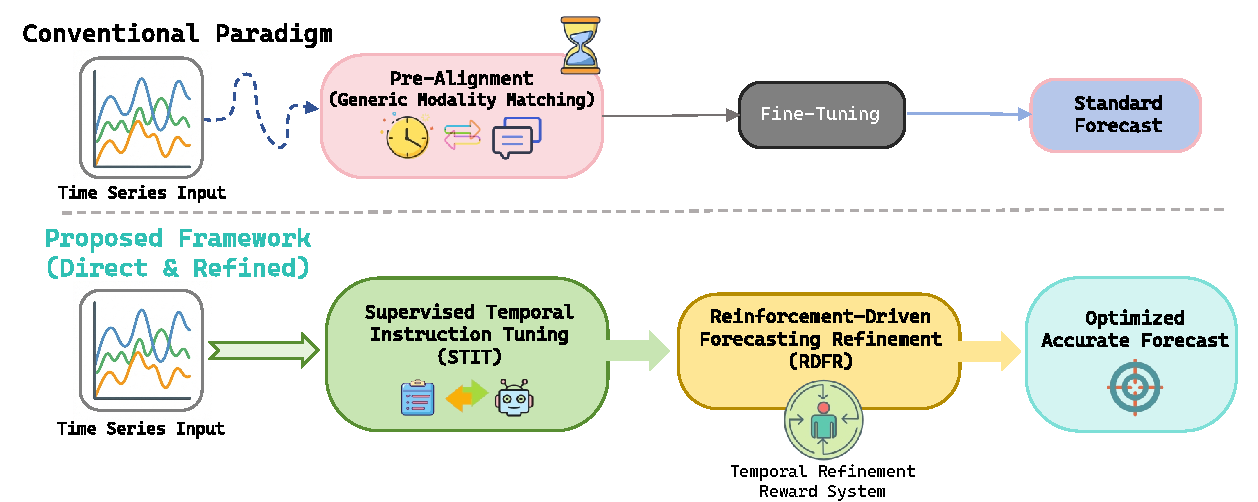
\includegraphics[width=0.75\linewidth]{figures/Intro.pdf}

  \caption{Comparison of forecasting paradigms. Conventional approaches~\cite{zhou2023one,jin2024timellm} rely on pre-alignment modules with limitations of granularity mismatch and architectural overhead to bridge modality gaps, when our proposed framework \textbf{RDTU} adopts a direct unification strategy, bypassing pre-alignment via \textbf{Supervised Temporal Instruction Tuning (STIT)} and strictly enforcing precision through \textbf{Reinforcement-Driven Forecasting Refinement (RDFR)}.}
  \label{fig:intro_paradigm}

\end{figure}


To overcome alignment limitations, we explore a paradigm that views forecasting as a native token generation task, treating numerical values directly as textual strings within unified prompts to bypass external encoders projecting continuous time series data into a high-dimensional semantic space. However, this direct approach faces two critical hurdles: \textbf{precision misalignment}, where standard causal modeling prioritizes semantic plausibility over the rigorous numerical accuracy required for regression, and \textbf{structural hallucinations}, where off-the-shelf models frequently fail to adhere to strict output formats or sequence lengths, rendering predictions unusable for downstream applications.

To address these challenges and fully leverage the native reasoning of LLMs, we propose the \textbf{Reinforced Direct Temporal Unification (RDTU)} framework. RDTU bridges the gap between discrete textual generation and continuous numerical forecasting through a progressive pipeline. Specifically, we first introduce \textbf{Supervised Temporal Instruction Tuning (STIT)} to align the model with the structure of time-series prompts. Crucially, to tackle the precision and formatting challenges inherent in textual token generation, we design a \textbf{Reinforcement-Driven Forecasting Refinement (RDFR)} mechanism. This stage employs a specialized reward system to rigorously enforce numerical accuracy and syntactic validity, ensuring the LLM acts as a precise forecaster. The following empirical evaluations confirm that this streamlined approach yields State-of-the-Art results while simplifying the training process. Our main contributions are summarized as follows:

\begin{itemize}
    \item We propose \textbf{STIT}, a direct unification paradigm that bypasses auxiliary pre-alignment by treating time series as native text which not only simplifies training complexity but also achieves robust instruction adherence and comparable forecasting performance.

    \item We introduce \textbf{RDFR}, a specialized reinforcement learning system utilizing dual-stream hard sample mining and multi-objective rewards which bridges the gap between discrete generation and continuous precision.

    \item We validate the efficacy of our progressive \textbf{RDTU} framework through extensive experiments. Results demonstrate that this synergy yields superior accuracy and generalization.

\end{itemize}

\FloatBarrier\needspace{10\baselineskip}\section{Related Works}

RDTU studies direct numerical text generation with supervised instruction tuning and reinforcement-driven refinement for time series forecasting. In the following, we review existing literature across two key dimensions: traditional Transformer-based approaches and emerging LLM-based methodologies for time series forecasting (TSF).


\paragraph{Transformer-based TSF}
Deep learning architectures have fundamentally reshaped time series forecasting, with Transformers initially gaining prominence due to their sequence modeling capabilities~\citep{wen2022transformers}. To address computational bottlenecks, efficient variants such as Informer~\citep{zhou2021informer}, Reformer~\citep{kitaev2020reformer}, and Pyraformer~\citep{liu2022pyraformer} introduced sparse attention mechanisms to reduce complexity for long-sequence modeling. Subsequently, decomposition-based architectures like Autoformer~\citep{wu2021autoformer} and FEDformer~\citep{zhou2022fedformer} enhanced stability on non-stationary data by explicitly disentangling seasonal and trend components. Most recently, PatchTST~\citep{nie2022time} and iTransformer~\citep{liu2023itransformer} have achieved state-of-the-art results by employing patching techniques and inverted embeddings to effectively capture multivariate correlations and local semantic contexts.


\paragraph{LLM-based TSF}

The unprecedented capabilities of foundation models have catalyzed cross-modality learning in time series, evolving from the zero-shot textual generation of LLMTime~\citep{gruver2023llmtime} to alignment-based adaptations. Notably, GPT4TS~\citep{zhou2023one} validates freezing LLM backbones with fine-tuned embeddings, while Time-LLM~\citep{jin2024timellm} employs a reprogramming framework to align temporal patches with text prototypes, and UniTime~\citep{liu2024unitime} utilizes textual instructions for cross-domain unification. Concurrently, research has expanded into visual modalities: VisionTS~\citep{chen2024visionts} adapts masked autoencoders for zero-shot forecasting by treating time series as visual signals; Time-VLM~\citep{zhong2025time} leverages vision-language models by converting data into visual plots; and DMMV-A~\citep{shen2025dmmv} enhances large vision models through multi-view constraints to optimize long-term forecasting stability. Beyond adapting general-purpose LLMs, recent studies have also explored dedicated time-series foundation models pre-trained on large-scale temporal corpora, such as Chronos-2, TimesFM, Moirai, and MOMENT~\citep{ansari2025chronos2,das2024decoder,woo2024unified,goswami2024moment}.

\FloatBarrier\needspace{10\baselineskip}\input{sections/3_methodology}
\FloatBarrier\needspace{10\baselineskip}\section{Main Results}

\begin{table}[H]\centering\small
\caption{Long-term forecasting: horizon averages. Each entry is MSE / MAE; lower values are better.}\label{tab:long-term-forecasting-brief}
\begin{minipage}[t]{0.48\linewidth}\vspace{0pt}\centering\small
\textbf{ETTh1}\par\smallskip
\begin{tabular}{lr}\toprule Model & MSE / MAE\\\midrule
\rowcolor{blue!5}
\textbf{RDTU} & \textbf{0.399 / 0.413}\\
GPT4TS & 0.418 / 0.421\\
Time-LLM & 0.418 / 0.432\\
DMMV-A & 0.395 / 0.414\\
Time-VLM & 0.405 / 0.420\\
VisionTS & 0.407 / 0.419\\
PatchTST & 0.413 / 0.431\\
CycleNet & 0.415 / 0.426\\
TimesNet & 0.458 / 0.450\\
DLinear & 0.423 / 0.430\\
FEDformer & 0.440 / 0.460\\
\bottomrule\end{tabular}\end{minipage}\hfill\begin{minipage}[t]{0.48\linewidth}\vspace{0pt}\centering\small
\textbf{ETTh2}\par\smallskip
\begin{tabular}{lr}\toprule Model & MSE / MAE\\\midrule
\rowcolor{blue!5}
\textbf{RDTU} & \textbf{0.337 / 0.377}\\
GPT4TS & 0.354 / 0.389\\
Time-LLM & 0.361 / 0.396\\
DMMV-A & 0.337 / 0.388\\
Time-VLM & 0.341 / 0.391\\
VisionTS & 0.351 / 0.386\\
PatchTST & 0.330 / 0.379\\
CycleNet & 0.355 / 0.398\\
TimesNet & 0.414 / 0.427\\
DLinear & 0.431 / 0.447\\
FEDformer & 0.437 / 0.449\\
\bottomrule\end{tabular}\end{minipage}
\end{table}
\begin{table}[H]\centering\small
\caption*{Table S1 (continued).}
\begin{minipage}[t]{0.48\linewidth}\vspace{0pt}\centering\small
\textbf{ETTm1}\par\smallskip
\begin{tabular}{lr}\toprule Model & MSE / MAE\\\midrule
\rowcolor{blue!5}
\textbf{RDTU} & \textbf{0.340 / 0.367}\\
GPT4TS & 0.363 / 0.378\\
Time-LLM & 0.356 / 0.377\\
DMMV-A & 0.340 / 0.371\\
Time-VLM & 0.351 / 0.376\\
VisionTS & 0.344 / 0.373\\
PatchTST & 0.351 / 0.381\\
CycleNet & 0.355 / 0.379\\
TimesNet & 0.400 / 0.406\\
DLinear & 0.357 / 0.379\\
FEDformer & 0.448 / 0.452\\
\bottomrule\end{tabular}\end{minipage}\hfill\begin{minipage}[t]{0.48\linewidth}\vspace{0pt}\centering\small
\textbf{ETTm2}\par\smallskip
\begin{tabular}{lr}\toprule Model & MSE / MAE\\\midrule
\rowcolor{blue!5}
\textbf{RDTU} & \textbf{0.250 / 0.309}\\
GPT4TS & 0.254 / 0.311\\
Time-LLM & 0.261 / 0.316\\
DMMV-A & 0.256 / 0.317\\
Time-VLM & 0.248 / 0.311\\
VisionTS & 0.267 / 0.327\\
PatchTST & 0.255 / 0.315\\
CycleNet & 0.251 / 0.309\\
TimesNet & 0.291 / 0.333\\
DLinear & 0.267 / 0.332\\
FEDformer & 0.305 / 0.349\\
\bottomrule\end{tabular}\end{minipage}
\end{table}
\begin{table}[H]\centering\small
\caption*{Table S1 (continued).}
\begin{minipage}[t]{0.48\linewidth}\vspace{0pt}\centering\small
\textbf{Illness}\par\smallskip
\begin{tabular}{lr}\toprule Model & MSE / MAE\\\midrule
\rowcolor{blue!5}
\textbf{RDTU} & \textbf{1.559 / 0.812}\\
GPT4TS & 1.871 / 0.852\\
Time-LLM & 2.018 / 0.894\\
DMMV-A & 1.407 / 0.771\\
Time-VLM & --\\
VisionTS & 1.482 / 0.796\\
PatchTST & 1.443 / 0.798\\
CycleNet & 2.187 / 0.992\\
TimesNet & 2.139 / 0.931\\
DLinear & 2.169 / 1.041\\
FEDformer & 2.847 / 1.144\\
\bottomrule\end{tabular}\end{minipage}\hfill\begin{minipage}[t]{0.48\linewidth}\vspace{0pt}\centering\small
\textbf{Electricity}\par\smallskip
\begin{tabular}{lr}\toprule Model & MSE / MAE\\\midrule
\rowcolor{blue!5}
\textbf{RDTU} & \textbf{0.156 / 0.246}\\
GPT4TS & 0.170 / 0.263\\
Time-LLM & 0.165 / 0.259\\
DMMV-A & 0.158 / 0.248\\
Time-VLM & 0.172 / 0.272\\
VisionTS & 0.159 / 0.250\\
PatchTST & 0.162 / 0.253\\
CycleNet & 0.158 / 0.250\\
TimesNet & 0.193 / 0.295\\
DLinear & 0.166 / 0.264\\
FEDformer & 0.214 / 0.327\\
\bottomrule\end{tabular}\end{minipage}
\end{table}
\begin{table}[H]\centering\small
\caption*{Table S1 (continued).}
\begin{minipage}[t]{0.48\linewidth}\vspace{0pt}\centering\small
\textbf{Weather}\par\smallskip
\begin{tabular}{lr}\toprule Model & MSE / MAE\\\midrule
\rowcolor{blue!5}
\textbf{RDTU} & \textbf{0.221 / 0.251}\\
GPT4TS & 0.227 / 0.255\\
Time-LLM & 0.244 / 0.270\\
DMMV-A & 0.217 / 0.256\\
Time-VLM & 0.224 / 0.263\\
VisionTS & 0.225 / 0.258\\
PatchTST & 0.226 / 0.264\\
CycleNet & 0.242 / 0.278\\
TimesNet & 0.259 / 0.287\\
DLinear & 0.249 / 0.300\\
FEDformer & 0.309 / 0.360\\
\bottomrule\end{tabular}\end{minipage}\hfill\begin{minipage}[t]{0.48\linewidth}\vspace{0pt}\centering\small
\textbf{Traffic}\par\smallskip
\begin{tabular}{lr}\toprule Model & MSE / MAE\\\midrule
\rowcolor{blue!5}
\textbf{RDTU} & \textbf{0.389 / 0.255}\\
GPT4TS & 0.421 / 0.274\\
Time-LLM & 0.422 / 0.281\\
DMMV-A & 0.389 / 0.257\\
Time-VLM & 0.419 / 0.304\\
VisionTS & 0.386 / 0.256\\
PatchTST & 0.391 / 0.264\\
CycleNet & 0.421 / 0.289\\
TimesNet & 0.620 / 0.336\\
DLinear & 0.434 / 0.295\\
FEDformer & 0.610 / 0.376\\
\bottomrule\end{tabular}\end{minipage}
\end{table}
\noindent\textbf{Source-reported ranking counts.} RDTU: 9, GPT4TS: 0, Time-LLM: 0, DMMV-A: 5, Time-VLM: 1, VisionTS: 1, PatchTST: 1, CycleNet: 1, TimesNet: 0, DLinear: 0, FEDformer: 0. The original counting convention is not specified; these values are retained without recalculation.\par

\begin{table}[H]\centering\small
\caption{M4 forecasting: weighted averages. Lower values are better.}\label{tab:short-term-forecasting-brief}
\textbf{Average}\par\smallskip
\begin{adjustbox}{max width=\linewidth}\begin{tabular}{lrrr}\toprule
\textbf{Model} & \textbf{SMAPE} & \textbf{MASE} & \textbf{OWA}\\\midrule
\rowcolor{blue!5}
\textbf{RDTU} & \textbf{11.979} & \textbf{1.599} & \textbf{0.859}\\
Time-LLM & 11.983 & 1.595 & 0.859\\
GPT4TS & 12.69 & 1.808 & 0.94\\
TimesNet & 12.88 & 1.836 & 0.955\\
PatchTST & 12.059 & 1.623 & 0.869\\
N-HiTS & 12.035 & 1.625 & 0.869\\
N-BEATS & 12.25 & 1.698 & 0.896\\
ETSformer & 14.718 & 2.408 & 1.172\\
LightTS & 13.525 & 2.111 & 1.051\\
DLinear & 13.639 & 2.095 & 1.051\\
FEDformer & 13.16 & 1.775 & 0.949\\
Stationary & 12.780 & 1.756 & 0.930\\
Autoformer & 12.909 & 1.771 & 0.939\\
Informer & 14.086 & 2.718 & 1.230\\
Reformer & 18.200 & 4.223 & 1.775\\
\bottomrule\end{tabular}\end{adjustbox}\end{table}


\noindent \textbf{Datasets.} We adopt 8 widely used MTS benchmarks: ETT (Electricity Transformer Temperature) \cite{zhou2021informer}, including ETTh1, ETTh2, ETTm1, ETTm2; Weather \cite{wu2021autoformer}, Illness \cite{wu2021autoformer}, Traffic \cite{wu2021autoformer}, and Electricity \cite{electricity}, which have been extensively adopted for benchmarking long-term forecasting models~\citep{wu2022timesnet}.
The prediction horizon $H$ is set to \{24, 36, 48, 60\} for Illness, and \{96, 192, 336, 720\} for the remaining datasets.

\noindent \textbf{Baselines.} We compare \method{} with SOTA methods, categorized as follows:
(1) \textbf{VLM-based models:} \texttt{Time-VLM}~\cite{zhong2025time};
(2) \textbf{LVM-based models:} \texttt{VisionTS}~\cite{chen2024visionts} and \texttt{DMMV-A}~\cite{shen2025dmmv};
(3) \textbf{LLM-based models:} \texttt{Time-LLM}~\cite{jin2024timellm} and \texttt{GPT4TS}~\cite{zhou2023one};
(4) \textbf{Transformer-based models:} \texttt{PatchTST}~\cite{nie2022time}, \texttt{FEDformer}~\cite{zhou2022fedformer}, \texttt{Autoformer}~\cite{wu2021autoformer}, \texttt{Stationary}~\cite{liu2022non}, \texttt{ETSformer}~\cite{woo2022etsformer}, and \texttt{Informer}~\cite{zhou2021informer};
(5) \textbf{Non-Transformer models:} \texttt{DLinear}~\cite{zeng2023transformers}, \texttt{TimesNet}~\cite{wu2022timesnet}, and \texttt{CycleNet}~\cite{lin2024cyclenet}.
In short-term forecasting, we compare our model with N-HiTS~\cite{challu2023nhits} and N-BEATS~\cite{oreshkin2019n}.

\noindent \textbf{Implementation.} We implement our framework using \textbf{Qwen2.5-7B-Instruct}~\citep{qwen2.5} as the primary backbone.

All experiments are conducted on 8 \textbf{NVIDIA A100 (80GB)} GPUs. More details such as specific training expenses are shown in \shortautoref{appx:implementation}.

\subsection{Long-term Forecasting} \label{sec:long-term-forecasting}

\noindent\textbf{Setups.} We conduct extensive evaluations on eight widely-used real-world benchmarks: ETTh1, ETTh2, ETTm1, ETTm2, Weather, Electricity (ECL), Traffic, and ILI.

\noindent\textbf{Results.} \shortautoref{tab:long-term-forecasting-brief} summarizes the long-term forecasting performance. \textbf{RDTU} achieves superior accuracy, securing the highest number of best results (\textbf{9 wins}) across all benchmarks. It achieves highly competitive state-of-the-art-level performance, while remaining competitive with the strongest specialized numerical and vision-based baselines. Notably, RDTU establishes a significant lead over the strongest language-based baselines, reducing MSE by approximately \textbf{5.5\%} compared to Time-LLM on the \textit{Electricity} dataset and \textbf{4.5\%} versus GPT4TS on \textit{ETTh1}. These results confirm that our direct unification strategy, devoid of alignment bottlenecks, captures complex temporal dependencies with greater precision than competing paradigms.

\subsection{Short-term Forecasting}

\noindent\textbf{Setups.} We extend our evaluation to short-term forecasting using the M4 benchmark~\citep{makridakis2018m4}.

We employ Symmetric Mean Absolute Percentage Error (SMAPE), Mean Absolute Scaled Error (MASE), and Overall Weighted Average (OWA) as the evaluation metrics.

\noindent\textbf{Results.} As presented in \shortautoref{tab:short-term-forecasting-brief}, \textbf{RDTU} demonstrates robust short-horizon performance, achieving the lowest SMAPE of \textbf{11.979} and a state-of-the-art OWA of \textbf{0.859}. It significantly outperforms baselines like GPT4TS (OWA 0.940) and TimesNet (OWA 0.955), proving that our skip-alignment strategy effectively preserves local temporal details. Furthermore, RDTU surpasses specialized models such as N-HiTS and PatchTST (both OWA 0.869). While matching Time-LLM's competitive performance, RDTU achieves these results via a more streamlined direct unification architecture, validating the efficacy of the RDFR system in optimizing precision across varying temporal scales.

\begin{table}[H]\centering\small
\caption{Few-shot forecasting: 10\% horizon averages. Each entry is MSE / MAE; lower values are better.}\label{tab:few-shot-forecasting-10per-brief}
\begin{minipage}[t]{0.48\linewidth}\vspace{0pt}\centering\small
\textbf{ETTh1}\par\smallskip
\begin{tabular}{lr}\toprule Model & MSE / MAE\\\midrule
\rowcolor{blue!5}
\textbf{RDTU} & \textbf{0.551 / 0.513}\\
Time-LLM & 0.556 / 0.522\\
GPT4TS & 0.590 / 0.525\\
DLinear & 0.691 / 0.600\\
PatchTST & 0.633 / 0.542\\
TimesNet & 0.869 / 0.628\\
FEDformer & 0.639 / 0.561\\
Autoformer & 0.702 / 0.596\\
Stationary & 0.915 / 0.639\\
ETSformer & 1.180 / 0.834\\
LightTS & 1.375 / 0.877\\
Informer & 1.199 / 0.809\\
Reformer & 1.249 / 0.833\\
\bottomrule\end{tabular}\end{minipage}\hfill\begin{minipage}[t]{0.48\linewidth}\vspace{0pt}\centering\small
\textbf{ETTh2}\par\smallskip
\begin{tabular}{lr}\toprule Model & MSE / MAE\\\midrule
\rowcolor{blue!5}
\textbf{RDTU} & \textbf{0.367 / 0.389}\\
Time-LLM & 0.370 / 0.394\\
GPT4TS & 0.397 / 0.421\\
DLinear & 0.605 / 0.538\\
PatchTST & 0.415 / 0.431\\
TimesNet & 0.479 / 0.465\\
FEDformer & 0.466 / 0.475\\
Autoformer & 0.488 / 0.499\\
Stationary & 0.462 / 0.455\\
ETSformer & 0.894 / 0.713\\
LightTS & 2.655 / 1.160\\
Informer & 3.872 / 1.513\\
Reformer & 3.485 / 1.486\\
\bottomrule\end{tabular}\end{minipage}
\end{table}
\begin{table}[H]\centering\small
\caption*{Table S3 (continued).}
\begin{minipage}[t]{0.48\linewidth}\vspace{0pt}\centering\small
\textbf{ETTm1}\par\smallskip
\begin{tabular}{lr}\toprule Model & MSE / MAE\\\midrule
\rowcolor{blue!5}
\textbf{RDTU} & \textbf{0.402 / 0.424}\\
Time-LLM & 0.404 / 0.427\\
GPT4TS & 0.464 / 0.441\\
DLinear & 0.411 / 0.429\\
PatchTST & 0.501 / 0.466\\
TimesNet & 0.677 / 0.537\\
FEDformer & 0.722 / 0.605\\
Autoformer & 0.802 / 0.628\\
Stationary & 0.797 / 0.578\\
ETSformer & 0.980 / 0.714\\
LightTS & 0.971 / 0.705\\
Informer & 1.192 / 0.821\\
Reformer & 1.426 / 0.856\\
\bottomrule\end{tabular}\end{minipage}\hfill\begin{minipage}[t]{0.48\linewidth}\vspace{0pt}\centering\small
\textbf{ETTm2}\par\smallskip
\begin{tabular}{lr}\toprule Model & MSE / MAE\\\midrule
\rowcolor{blue!5}
\textbf{RDTU} & \textbf{0.274 / 0.319}\\
Time-LLM & 0.277 / 0.323\\
GPT4TS & 0.293 / 0.335\\
DLinear & 0.316 / 0.368\\
PatchTST & 0.296 / 0.343\\
TimesNet & 0.320 / 0.353\\
FEDformer & 0.463 / 0.488\\
Autoformer & 1.342 / 0.930\\
Stationary & 0.332 / 0.366\\
ETSformer & 0.447 / 0.487\\
LightTS & 0.987 / 0.756\\
Informer & 3.370 / 1.440\\
Reformer & 3.978 / 1.587\\
\bottomrule\end{tabular}\end{minipage}
\end{table}
\begin{table}[H]\centering\small
\caption*{Table S3 (continued).}
\begin{minipage}[t]{0.48\linewidth}\vspace{0pt}\centering\small
\textbf{Weather}\par\smallskip
\begin{tabular}{lr}\toprule Model & MSE / MAE\\\midrule
\rowcolor{blue!5}
\textbf{RDTU} & \textbf{0.232 / 0.270}\\
Time-LLM & 0.234 / 0.273\\
GPT4TS & 0.238 / 0.275\\
DLinear & 0.241 / 0.283\\
PatchTST & 0.242 / 0.279\\
TimesNet & 0.279 / 0.301\\
FEDformer & 0.284 / 0.324\\
Autoformer & 0.300 / 0.342\\
Stationary & 0.318 / 0.323\\
ETSformer & 0.318 / 0.360\\
LightTS & 0.289 / 0.322\\
Informer & 0.597 / 0.495\\
Reformer & 0.546 / 0.469\\
\bottomrule\end{tabular}\end{minipage}\hfill\begin{minipage}[t]{0.48\linewidth}\vspace{0pt}\centering\small
\textbf{Electricity}\par\smallskip
\begin{tabular}{lr}\toprule Model & MSE / MAE\\\midrule
\rowcolor{blue!5}
\textbf{RDTU} & \textbf{0.173 / 0.268}\\
Time-LLM & 0.175 / 0.270\\
GPT4TS & 0.176 / 0.269\\
DLinear & 0.180 / 0.280\\
PatchTST & 0.180 / 0.273\\
TimesNet & 0.323 / 0.392\\
FEDformer & 0.346 / 0.427\\
Autoformer & 0.431 / 0.478\\
Stationary & 0.444 / 0.480\\
ETSformer & 0.660 / 0.617\\
LightTS & 0.441 / 0.489\\
Informer & 1.195 / 0.891\\
Reformer & 0.965 / 0.768\\
\bottomrule\end{tabular}\end{minipage}
\end{table}
\begin{table}[H]\centering\small
\caption*{Table S3 (continued).}
\begin{minipage}[t]{0.48\linewidth}\vspace{0pt}\centering\small
\textbf{Traffic}\par\smallskip
\begin{tabular}{lr}\toprule Model & MSE / MAE\\\midrule
\rowcolor{blue!5}
\textbf{RDTU} & \textbf{0.426 / 0.303}\\
Time-LLM & 0.429 / 0.306\\
GPT4TS & 0.440 / 0.310\\
DLinear & 0.447 / 0.313\\
PatchTST & 0.430 / 0.305\\
TimesNet & 0.951 / 0.535\\
FEDformer & 0.663 / 0.425\\
Autoformer & 0.749 / 0.446\\
Stationary & 1.453 / 0.815\\
ETSformer & 1.914 / 0.936\\
LightTS & 1.248 / 0.684\\
Informer & 1.534 / 0.811\\
Reformer & 1.551 / 0.821\\
\bottomrule\end{tabular}\end{minipage}
\end{table}
\noindent\textbf{Source-reported ranking counts.} RDTU: 14, Time-LLM: 0, GPT4TS: 0, DLinear: 0, PatchTST: 0, TimesNet: 0, FEDformer: 0, Autoformer: 0, Stationary: 0, ETSformer: 0, LightTS: 0, Informer: 0, Reformer: 0. The original counting convention is not specified; these values are retained without recalculation.\par

\begin{table}[H]\centering\small
\caption{Zero-shot ETT transfer: horizon averages. Each entry is MSE / MAE; lower values are better.}\label{tab:zero-shot-forecasting-brief}
\begin{minipage}[t]{0.48\linewidth}\vspace{0pt}\centering\small
\textbf{ETTh1 $\to$ ETTh2}\par\smallskip
\begin{tabular}{lr}\toprule Model & MSE / MAE\\\midrule
\rowcolor{blue!5}
\textbf{RDTU} & \textbf{0.344 / 0.379}\\
Time-LLM & 0.353 / 0.387\\
LLMTime & 0.992 / 0.708\\
GPT4TS & 0.406 / 0.422\\
DLinear & 0.493 / 0.488\\
PatchTST & 0.380 / 0.405\\
TimesNet & 0.421 / 0.431\\
Autoformer & 0.582 / 0.548\\
\bottomrule\end{tabular}\end{minipage}\hfill\begin{minipage}[t]{0.48\linewidth}\vspace{0pt}\centering\small
\textbf{ETTh1 $\to$ ETTm2}\par\smallskip
\begin{tabular}{lr}\toprule Model & MSE / MAE\\\midrule
\rowcolor{blue!5}
\textbf{RDTU} & \textbf{0.266 / 0.333}\\
Time-LLM & 0.273 / 0.340\\
LLMTime & 1.867 / 0.869\\
GPT4TS & 0.325 / 0.363\\
DLinear & 0.415 / 0.452\\
PatchTST & 0.314 / 0.360\\
TimesNet & 0.327 / 0.361\\
Autoformer & 0.457 / 0.483\\
\bottomrule\end{tabular}\end{minipage}
\end{table}
\begin{table}[H]\centering\small
\caption*{Table S4 (continued).}
\begin{minipage}[t]{0.48\linewidth}\vspace{0pt}\centering\small
\textbf{ETTh2 $\to$ ETTh1}\par\smallskip
\begin{tabular}{lr}\toprule Model & MSE / MAE\\\midrule
\rowcolor{blue!5}
\textbf{RDTU} & \textbf{0.480 / 0.471}\\
Time-LLM & 0.479 / 0.474\\
LLMTime & 1.961 / 0.981\\
GPT4TS & 0.757 / 0.578\\
DLinear & 0.703 / 0.574\\
PatchTST & 0.565 / 0.513\\
TimesNet & 0.865 / 0.621\\
Autoformer & 0.757 / 0.608\\
\bottomrule\end{tabular}\end{minipage}\hfill\begin{minipage}[t]{0.48\linewidth}\vspace{0pt}\centering\small
\textbf{ETTh2 $\to$ ETTm2}\par\smallskip
\begin{tabular}{lr}\toprule Model & MSE / MAE\\\midrule
\rowcolor{blue!5}
\textbf{RDTU} & \textbf{0.268 / 0.329}\\
Time-LLM & 0.272 / 0.341\\
LLMTime & 1.867 / 0.869\\
GPT4TS & 0.335 / 0.370\\
DLinear & 0.328 / 0.386\\
PatchTST & 0.325 / 0.365\\
TimesNet & 0.342 / 0.376\\
Autoformer & 0.366 / 0.411\\
\bottomrule\end{tabular}\end{minipage}
\end{table}
\begin{table}[H]\centering\small
\caption*{Table S4 (continued).}
\begin{minipage}[t]{0.48\linewidth}\vspace{0pt}\centering\small
\textbf{ETTm1 $\to$ ETTh2}\par\smallskip
\begin{tabular}{lr}\toprule Model & MSE / MAE\\\midrule
\rowcolor{blue!5}
\textbf{RDTU} & \textbf{0.378 / 0.408}\\
Time-LLM & 0.381 / 0.412\\
LLMTime & 0.992 / 0.708\\
GPT4TS & 0.433 / 0.439\\
DLinear & 0.464 / 0.475\\
PatchTST & 0.439 / 0.438\\
TimesNet & 0.457 / 0.454\\
Autoformer & 0.470 / 0.479\\
\bottomrule\end{tabular}\end{minipage}\hfill\begin{minipage}[t]{0.48\linewidth}\vspace{0pt}\centering\small
\textbf{ETTm1 $\to$ ETTm2}\par\smallskip
\begin{tabular}{lr}\toprule Model & MSE / MAE\\\midrule
\rowcolor{blue!5}
\textbf{RDTU} & \textbf{0.261 / 0.316}\\
Time-LLM & 0.268 / 0.320\\
LLMTime & 1.867 / 0.869\\
GPT4TS & 0.313 / 0.348\\
DLinear & 0.335 / 0.389\\
PatchTST & 0.296 / 0.334\\
TimesNet & 0.322 / 0.354\\
Autoformer & 0.469 / 0.484\\
\bottomrule\end{tabular}\end{minipage}
\end{table}
\begin{table}[H]\centering\small
\caption*{Table S4 (continued).}
\begin{minipage}[t]{0.48\linewidth}\vspace{0pt}\centering\small
\textbf{ETTm2 $\to$ ETTh2}\par\smallskip
\begin{tabular}{lr}\toprule Model & MSE / MAE\\\midrule
\rowcolor{blue!5}
\textbf{RDTU} & \textbf{0.351 / 0.395}\\
Time-LLM & 0.354 / 0.400\\
LLMTime & 0.992 / 0.708\\
GPT4TS & 0.435 / 0.443\\
DLinear & 0.455 / 0.471\\
PatchTST & 0.409 / 0.425\\
TimesNet & 0.435 / 0.443\\
Autoformer & 0.423 / 0.439\\
\bottomrule\end{tabular}\end{minipage}\hfill\begin{minipage}[t]{0.48\linewidth}\vspace{0pt}\centering\small
\textbf{ETTm2 $\to$ ETTm1}\par\smallskip
\begin{tabular}{lr}\toprule Model & MSE / MAE\\\midrule
\rowcolor{blue!5}
\textbf{RDTU} & \textbf{0.412 / 0.434}\\
Time-LLM & 0.414 / 0.438\\
LLMTime & 1.933 / 0.984\\
GPT4TS & 0.769 / 0.567\\
DLinear & 0.649 / 0.537\\
PatchTST & 0.568 / 0.492\\
TimesNet & 0.769 / 0.567\\
Autoformer & 0.755 / 0.591\\
\bottomrule\end{tabular}\end{minipage}
\end{table}


\subsection{Few-shot Forecasting}

\noindent\textbf{Setups.} LLMs have demonstrated remarkable few-shot learning capabilities~\citep{liu2023large}. To evaluate the data efficiency of our framework in low-resource scenarios, we conduct few-shot learning experiments by restricting the training set to only $10\%$ of the available data.

\noindent\textbf{Results.} As reported in \shortautoref{tab:few-shot-forecasting-10per-brief}, \textbf{RDTU} exhibits exceptional few-shot capabilities, securing the best performance across all metrics (14 out of 14). While data scarcity severely impacts deep learning baselines like PatchTST (ETTh1 MSE 0.633), RDTU maintains a robust MSE of \textbf{0.551} on the same task. Moreover, it consistently outperforms adapter-based LLMs such as Time-LLM (0.556) and GPT4TS (0.590). This validates that our direct unification strategy effectively leverages the pre-trained backbone to mitigate overfitting, proving superior efficiency over complex auxiliary adapters in data-limited scenarios.

\subsection{Zero-shot Forecasting}

\noindent\textbf{Setups.} To assess the generalization capability of our framework under distribution shifts, we conduct zero-shot learning experiments using the ETT dataset family.

\noindent\textbf{Results.} As reported in \shortautoref{tab:zero-shot-forecasting-brief}, \textbf{RDTU} demonstrates exceptional transferability, achieving the lowest horizon-averaged MSE in \textbf{7 of 8 transfer directions}. For $ETTh2 \to ETTh1$, RDTU obtains 0.480 MSE compared with 0.479 for Time-LLM, while its MAE is lower (0.471 versus 0.474). It highlights a fundamental advantage over supervised baselines, significantly outperforming Time-LLM in the $ETTh1 \to ETTh2$ transfer (MSE \textbf{0.344} vs. 0.353). Moreover, RDTU consistently surpasses competing LLM-based methods; in the challenging $ETTh2 \to ETTh1$ scenario, it maintains a robust MSE of \textbf{0.480}, far exceeding GPT4TS (0.757). These results support cross-dataset transfer within the evaluated ETT-family settings.

\subsection{Showcases Analysis}

\begin{figure}[htbp]\centering
\begin{subfigure}[t]{0.32\linewidth}\centering
\includegraphics[width=\linewidth]{figures/showcase/ground_truth_plot_01_len.pdf}\caption{Incomplete prediction (early stopping).}\label{fig:showcase01-len}\end{subfigure}%
\hfill%
\begin{subfigure}[t]{0.32\linewidth}\centering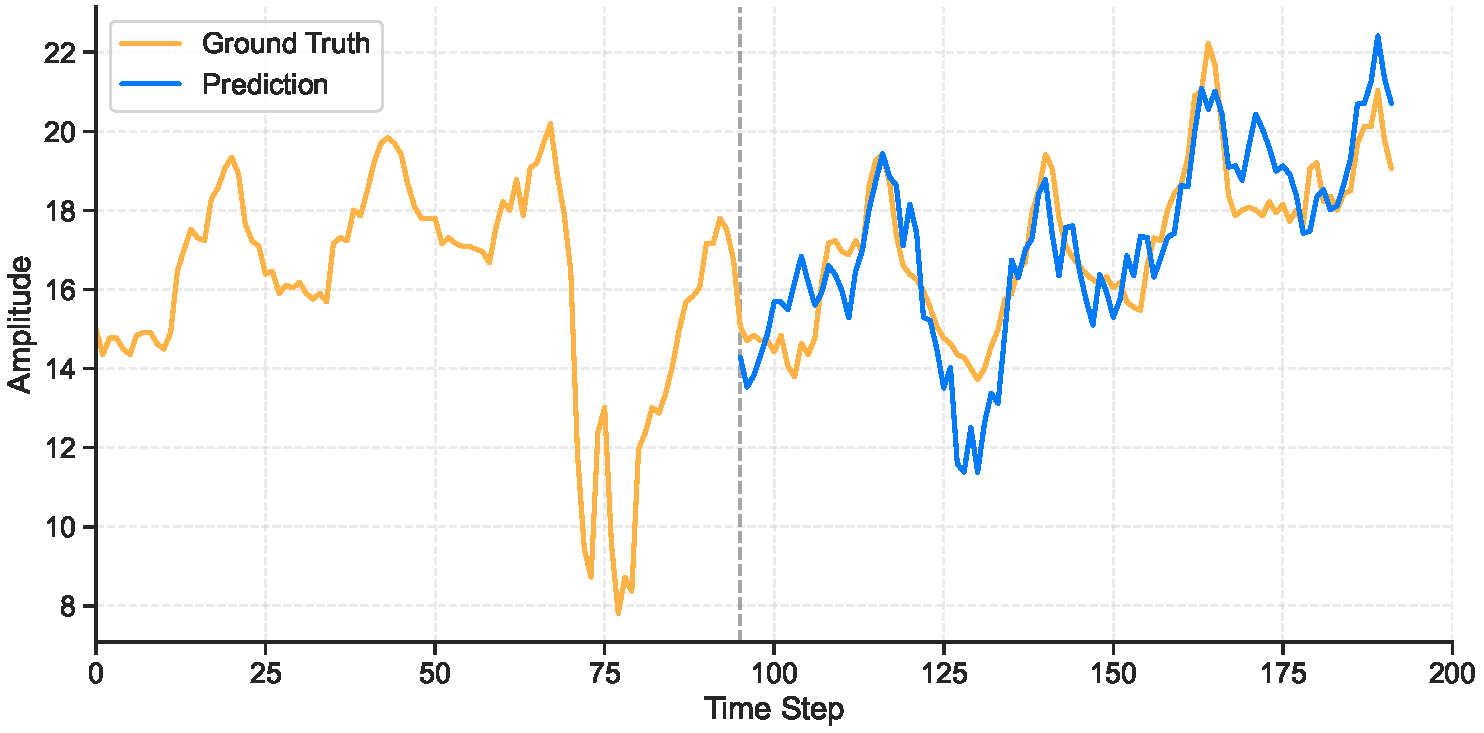
\includegraphics[width=\linewidth]{figures/showcase/ground_truth_plot_03_mse.pdf}\caption{Low prediction accuracy (high MSE).}\label{fig:showcase02-mse}\end{subfigure}%
\hfill%
\begin{subfigure}[t]{0.32\linewidth}\centering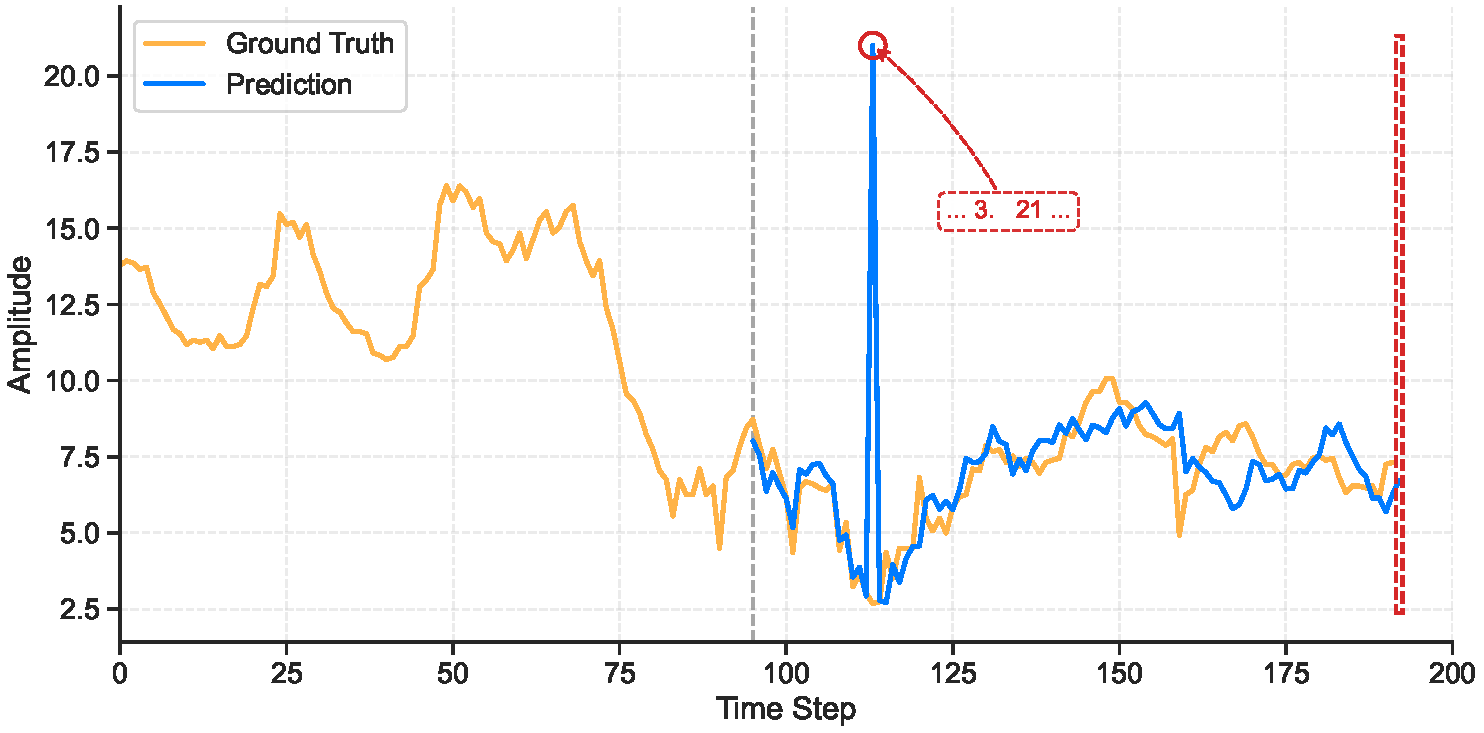
\includegraphics[width=\linewidth]{figures/showcase/ground_truth_plot_05_decimal.pdf}\caption{Formatting error causing abnormal spikes.}\label{fig:showcase03-fmt}\end{subfigure}%
\par\medskip
\begin{subfigure}[t]{0.32\linewidth}\centering
\includegraphics[width=\linewidth]{figures/showcase/ground_truth_plot_01.pdf}\caption{Correction of prediction length.}\label{fig:showcase01}\end{subfigure}%
\hfill%
\begin{subfigure}[t]{0.32\linewidth}\centering
\includegraphics[width=\linewidth]{figures/showcase/ground_truth_plot_03.pdf}\caption{Enhanced prediction precision.}\label{fig:showcase02}\end{subfigure}%
\hfill%
\begin{subfigure}[t]{0.32\linewidth}\centering
\includegraphics[width=\linewidth]{figures/showcase/ground_truth_plot_05.pdf}\caption{Rectification of output format and outliers.}\label{fig:showcase03}\end{subfigure}%

\caption{Showcase visualizations of input-96-predict-96 results on the ETTh1 dataset. The top row (a--c) displays the baseline performance of the STIT model, which exhibits limitations in sequence length, accuracy, and output formatting. The bottom row (d--f) shows the improvements achieved after applying the proposed RDFR framework. More showcases are provided in \shortautoref{appx:showcase_addition}.}\label{fig:showcases}\end{figure}


To intuitively understand how our proposed \textit{Temporal Refinement Reward System} in RDFR stage refines the model's behavior, we visualize a comparison between the STIT baseline and the final \method{} model in \shortautoref{fig:showcases}. This qualitative analysis targets three representative failure modes, validating the necessity of our composite reward system.

\textbf{Correction of Prediction Length}
As observed in \shortautoref{fig:showcase01-len}, the STIT model frequently suffers from "early stopping," failing to track the generation count and terminating the sequence before reaching the required horizon. This indicates a lack of internal counting logic. In contrast, \shortautoref{fig:showcase01} demonstrates the impact of the \textbf{Sequence Length Consistency Reward ($R_{len}$)}. By imposing a soft exponential length constraint, the RDFR stage forces the model to attend to the output length, ensuring the generated sequence perfectly matches the target horizon without truncation.

\textbf{Enhancement of Prediction Precision}
\shortautoref{fig:showcase02-mse} illustrates a case where the STIT model captures the general trend direction but fits loosely to the ground truth, exhibiting high variance and failing to capture local volatility. This corresponds to the limitations of token-level tuning in forecasting tasks. \shortautoref{fig:showcase02} showcases the refinement achieved via the \textbf{Prediction Accuracy Reward ($R_{acc}$)}. With its exponential scaling, $R_{acc}$ penalizes even minor deviations in the high-precision regime, driving the model to produce a curve that hugs the ground truth tightly and significantly reducing the MSE.

\textbf{Rectification of Formatting and Outliers}
Most critically, \shortautoref{fig:showcase03-fmt} reveals a severe "Integer Projection" hallucination where the STIT model fails to generate the decimal point (e.g., splitting a value like `3.21` into two tokens `3` and `21`). This formatting error inserts an extreme outlier into the time series and causes a phase shift in all subsequent data points. \shortautoref{fig:showcase03} confirms that the \textbf{Format Compliance Reward ($R_{fmt}$)} effectively eliminates this issue. By penalizing the model step-by-step for missing floating-point structures, the RDFR system enforces strict adherence to numerical syntax, restoring the smooth, continuous trajectory of the time series and preventing catastrophic outliers.

\subsection{Ablation and Sensitivity Analysis}
In this section, we perform comprehensive ablation studies to dissect the effectiveness of each component within the \method{} framework. Followed by \cite{jin2024timellm}, all experiments reported in this section are conducted on the \textbf{ETTh1} dataset with a fixed prediction horizon of $H=96$ unless otherwise explicitly stated.

\noindent\textbf{Component Analysis of the RDFR Framework.}\quad
To validate our design, we conducted an ablation study on the ETTh1 dataset. As shown in \shortautoref{tab:ablation_02}, while the off-the-shelf Qwen2.5-Instruct failed to generate valid outputs, the STIT model alone established a robust baseline with an MSE of \textbf{0.403}. This pivotal result demonstrates that complex pre-alignment modules are unnecessary; instruction tuning alone provides sufficient modality awareness for the LLM to function as a competent forecaster. Building on this foundation, the RDFR stage proved essential for precision. By imposing strict structural constraints and accuracy-driven rewards, the final RDTU framework further reduced the MSE to \textbf{0.351} with a \textbf{12.90\%} improvement over the STIT baseline, confirming that reinforcement learning effectively bridges the gap between basic instruction following and high-precision regression.

\input{tables/ablation02}

\begin{figure}[htbp]
    \centering

    \begin{subfigure}[t]{0.45\linewidth}
        \centering
        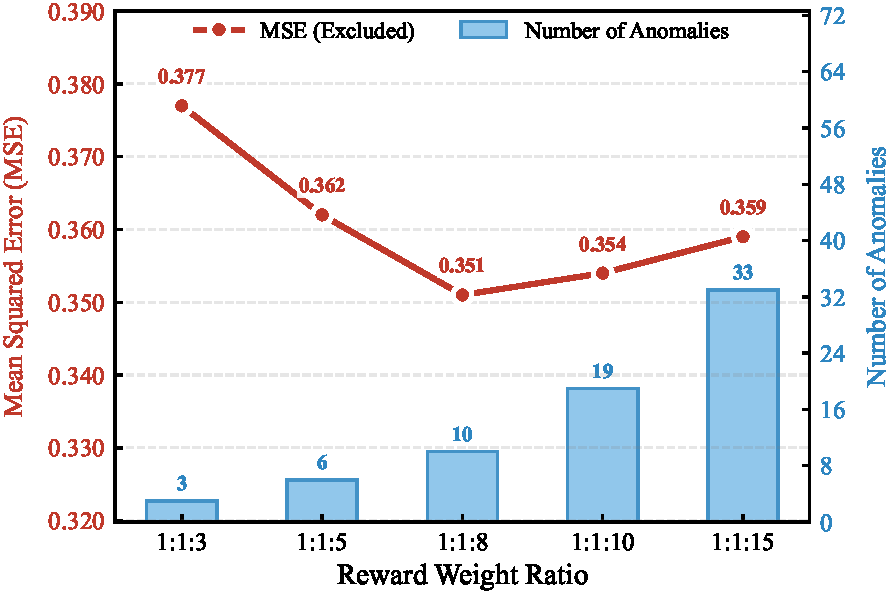
\includegraphics[width=\linewidth]{figures/ablation/ablation01.pdf}
        \caption{Impact of the reward weight ratio.}
        \label{fig:ablation_01}
    \end{subfigure}
    \hfill
    \begin{subfigure}[t]{0.52\linewidth}
        \centering
        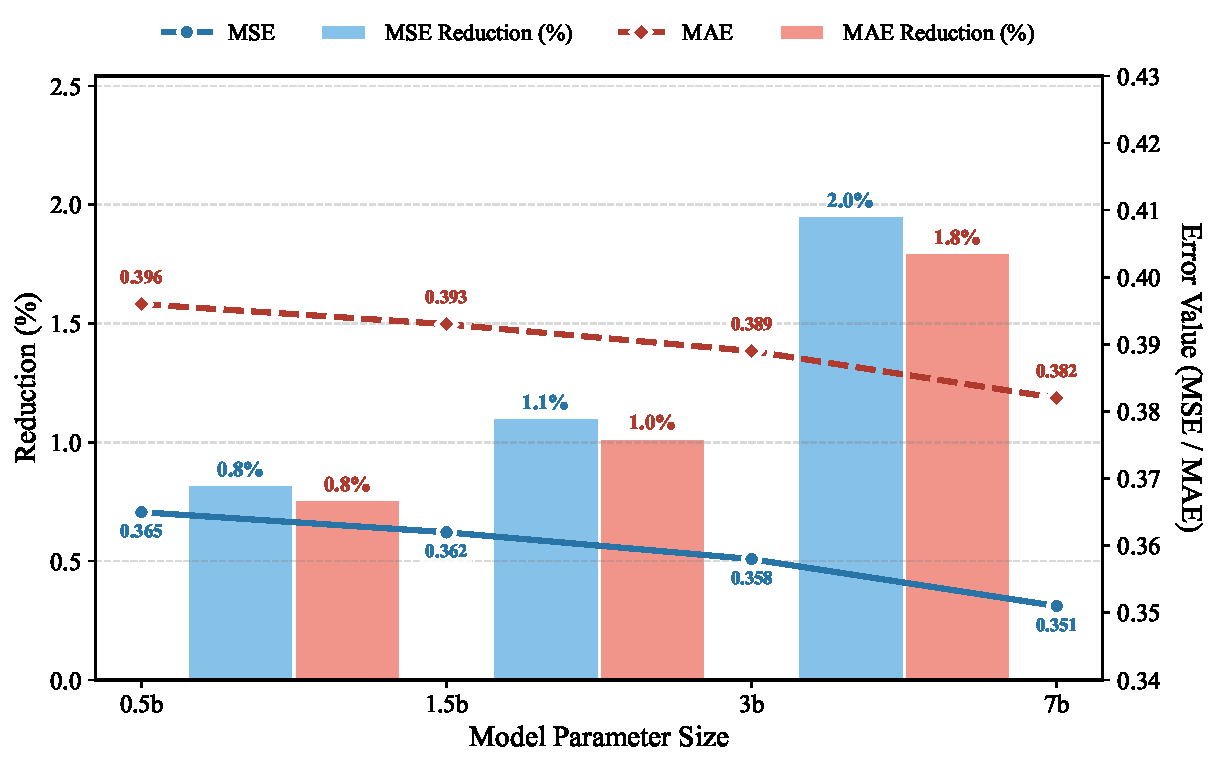
\includegraphics[width=\linewidth]{figures/ablation/ablation03_combined.pdf}
        \caption{Scaling laws on training efficiency and forecasting performance.}
        \label{fig:ablation_03}
    \end{subfigure}


    \caption{Ablation analysis of reward weighting and model scaling. Left: the red line represents the Mean Squared Error (MSE) on the excluded dataset, while the blue bars indicate the number of detected anomalies. Right: the line chart tracks MSE and MAE, showing that increased model capacity leads to consistent improvements in prediction accuracy.}
    \label{fig:ablation_combined}

\end{figure}


\noindent\textbf{Impact of Reward Weight Ratios.}\quad
We investigate the optimal balance between structural constraints and regression precision by varying the accuracy reward weight $\lambda_{acc}$ (fixing $\lambda_{len}:\lambda_{fmt}$ at $1:1$). Results on ETTh1 identify $\mathbf{1:1:8}$ as the optimal configuration, achieving the lowest MSE of \textbf{0.351}. Deviating from this equilibrium degrades performance via two distinct failure modes: low weights ($1:1:3$) result in under-optimization of numerical values (MSE 0.377), while excessive weights ($1:1:15$) induce "structural collapse." As shown in \shortautoref{fig:ablation_01}, pushing beyond the optimal threshold causes formatting anomalies to spike from 10 to 33, demonstrating that overpowering syntax constraints with accuracy objectives ultimately corrupts prediction validity.

\noindent\textbf{Impact of Model Scaling.}\quad
We evaluate the impact of model capacity across the Qwen2.5 family (0.5B, 1.5B, 3B, 7B). Results in \shortautoref{fig:ablation_03} reveal a robust scaling law: as parameter count increases, forecasting accuracy consistently improves, with MSE on ETTh1 monotonically decreasing from 0.365 (0.5B) to 0.351 (7B). This confirms that \textbf{RDTU} effectively harnesses the stronger reasoning capabilities of larger backbones to achieve finer precision.

\FloatBarrier\needspace{10\baselineskip}\section{Conclusion and Limitations}

In this paper, we proposed RDTU, a streamlined framework that directly formulates time series forecasting as a native token generation task without relying on complex pre-alignment modules. Through Supervised Temporal Instruction Tuning (STIT) for structure-aware forecasting adaptation and Reinforcement-Driven Forecasting Refinement (RDFR) for numerical precision and output validity, RDTU effectively transforms a general-purpose LLM into a reliable time series forecaster. Extensive experiments across long-term, short-term, few-shot, and zero-shot forecasting benchmarks demonstrate its strong accuracy and generalization ability. While RDTU achieves promising results on standard benchmarks, future work will further examine its robustness across broader real-world temporal domains.

\appendix
\FloatBarrier\needspace{10\baselineskip}\section{Experimental Details}\label{appx:implementation}

\subsection{Implementation}

For \textbf{Stage I (STIT)}, we utilize LoRA ($r=16, \alpha=32$) targeting query and value modules. Optimization is performed via AdamW (learning rate $2\times 10^{-4}$, global batch size 32) with a cosine annealing scheduler (0.03 warmup). In \textbf{Stage II (RDFR)}, we initialize the policy from the SFT checkpoint with a reduced learning rate of $5\times 10^{-6}$ and a KL-divergence coefficient $\beta_{kl}=0.04$. We configure the Group Size $G=8$, sampling 8 outputs per prompt. The total reward function $R_{total}$ combines length consistency ($R_{len}$), format compliance ($R_{fmt}$), and prediction accuracy ($R_{acc}$) with a strict ratio of 1:1:8 ($\lambda_{len}=0.1, \lambda_{fmt}=0.1, \lambda_{acc}=0.8$), prioritizing forecasting precision. Specifically, $R_{fmt}$ aggregates sub-goals (number, float, precision) with weights $\{0.2, 0.3, 0.5\}$, while sensitivity factors are set to $\alpha=0.5$ for length decay and $\beta=10.0$ for accuracy scaling.

\paragraph{Training Budget and Resource Usage.}
To further clarify the practical cost of the proposed two-stage training pipeline,
we report the per-dataset training budget and resource usage in Table~\ref{tab:training_resource}.
Although RDTU adopts a 7B LLM backbone, the overall training cost remains moderate.
For the STIT stage, training on standard long-term forecasting benchmarks requires only about 2.5--4.3 hours, with a peak memory usage of approximately 24 GB per GPU.
More importantly, the RDFR stage introduces only a small additional overhead, requiring about 0.3--0.5 hours and approximately 32 GB peak memory per GPU.
This confirms that the proposed reinforcement-driven refinement is a lightweight yet effective stage: it improves numerical precision and output validity without introducing extra pre-alignment modules or substantial architectural overhead.



\begin{table}[htbp]\centering\small
\caption{Training settings and resource usage on different datasets.}\label{tab:training_resource}
\setlength{\tabcolsep}{4pt}\renewcommand{\arraystretch}{1.25}
\begin{adjustbox}{max width=\linewidth}\begin{tabular}{lrrrrr}\toprule
\textbf{Dataset} & \textbf{Stage} & \textbf{Training size} & \textbf{Epochs} & \textbf{Hours} & \textbf{VRAM / GPU}\\\midrule
ETTh1 & STIT / RDFR & 8,545 / 425 & 15 / 3 & $\sim$2.5 / $\sim$0.3 & $\sim$24 GB / $\sim$32 GB\\
ETTh2 & STIT / RDFR & 8,545 / 425 & 15 / 3 & $\sim$2.5 / $\sim$0.3 & $\sim$24 GB / $\sim$32 GB\\
ETTm1 & STIT / RDFR & 34,465 / 1,713 & 5 / 2 & $\sim$4.3 / $\sim$0.5 & $\sim$24 GB / $\sim$32 GB\\
ETTm2 & STIT / RDFR & 34,465 / 1,713 & 5 / 2 & $\sim$4.3 / $\sim$0.5 & $\sim$24 GB / $\sim$32 GB\\
Electricity & STIT / RDFR & 18,317 / 911 & 8 / 3 & $\sim$3.7 / $\sim$0.5 & $\sim$24 GB / $\sim$32 GB\\
Traffic & STIT / RDFR & 12,185 / 606 & 10 / 3 & $\sim$3.0 / $\sim$0.3 & $\sim$24 GB / $\sim$32 GB\\
Weather & STIT / RDFR & 36,792 / 1,830 & 4 / 2 & $\sim$3.7 / $\sim$0.5 & $\sim$24 GB / $\sim$32 GB\\
\bottomrule\end{tabular}\end{adjustbox}\end{table}

\subsection{Evaluation Metrics}

For evaluation metrics, we utilize the mean square error (MSE) and mean absolute error (MAE) for long-term forecasting. In terms of the short-term forecasting on M4 benchmark, we adopt the symmetric mean absolute percentage error (SMAPE), mean absolute scaled error (MASE), and overall weighted average (OWA) as in N-BEATS \citep{oreshkin2019n}. Note that OWA is a specific metric utilized in the M4 competition. The calculations of these metrics are as follows:
\begin{align*} \label{equ:metrics}
    \text{MSE} &= \frac{1}{H}\sum_{h=1}^H (\mathbf{Y}_{h} - \Hat{\mathbf{Y}}_{h})^2,
    &
    \text{MAE} &= \frac{1}{H}\sum_{h=1}^H|\mathbf{Y}_{h} - \Hat{\mathbf{Y}}_{h}|,\\
    \text{SMAPE} &= \frac{200}{H} \sum_{h=1}^H \frac{|\mathbf{Y}_{h} - \Hat{\mathbf{Y}}_{h}|}{|\mathbf{Y}_{h}| + |\Hat{\mathbf{Y}}_{h}|},
    &
    \text{MAPE} &= \frac{100}{H} \sum_{h=1}^H \frac{|\mathbf{Y}_{h} - \Hat{\mathbf{Y}}_{h}|}{|\mathbf{Y}_{h}|}, \\
    \text{MASE} &= \frac{1}{H} \sum_{h=1}^H \frac{|\mathbf{Y}_{h} - \Hat{\mathbf{Y}}_{h}|}{\frac{1}{H-s}\sum_{j=s+1}^{H}|\mathbf{Y}_j - \mathbf{Y}_{j-s}|},
    &
    \text{OWA} &= \frac{1}{2} \left[ \frac{\text{SMAPE}}{\text{SMAPE}_{\textrm{Naïve2}}}  + \frac{\text{MASE}}{\text{MASE}_{\textrm{Naïve2}}}  \right],
\end{align*}
where $s$ is the periodicity of the time series data. $H$ denotes the number of data points (i.e., prediction horizon in our cases). $\mathbf{Y}_{h}$ and $\Hat{\mathbf{Y}}_{h}$ are the $h$-th ground truth and prediction where $h \in \{1, \cdots, H\}$.

\paragraph{Declaration of LLM Usage.}

LLMs are a core methodological component of this work. Specifically, we use Qwen2.5-Instruct as the backbone forecasting model and adapt it to time series forecasting through the proposed two-stage RDTU framework, including Supervised Temporal Instruction Tuning (STIT) and Reinforcement-Driven Forecasting Refinement (RDFR). The LLM is used to generate numerical time series predictions under structured prompts, while the training procedure, reward design, hyperparameters, and evaluation settings are documented in the paper and appendix.

\subsection{Dataset Details}

\begin{table}[htbp]\centering\small
\caption{Dataset statistics are from \citep{wu2022timesnet}. The dimension indicates the number of time series (i.e., channels), and the dataset size is organized in (training, validation, testing).}\label{tab:dataset}
\setlength{\tabcolsep}{4pt}\renewcommand{\arraystretch}{1.25}
\begin{adjustbox}{max width=\linewidth}\begin{tabular}{lrrrrr}\toprule
\textbf{Dataset} & \textbf{Dim.} & \textbf{Horizons} & \textbf{Train / val. / test} & \textbf{Frequency} & \textbf{Domain}\\\midrule
ETTm1 & 7 & [96, 192, 336, 720] & (34465, 11521, 11521) & 15 min & Temperature\\
ETTm2 & 7 & [96, 192, 336, 720] & (34465, 11521, 11521) & 15 min & Temperature\\
ETTh1 & 7 & [96, 192, 336, 720] & (8545, 2881, 2881) & 1 hour & Temperature\\
ETTh2 & 7 & [96, 192, 336, 720] & (8545, 2881, 2881) & 1 hour & Temperature\\
Electricity & 321 & [96, 192, 336, 720] & (18317, 2633, 5261) & 1 hour & Electricity\\
Traffic & 862 & [96, 192, 336, 720] & (12185, 1757, 3509) & 1 hour & Transportation\\
Weather & 21 & [96, 192, 336, 720] & (36792, 5271, 10540) & 10 min & Weather\\
ILI & 7 & [24, 36, 48, 60] & (617, 74, 170) & 1 week & Illness\\
M4-Yearly & 1 & 6 & (23000, 0, 23000) & Yearly & Demographic\\
M4-Quarterly & 1 & 8 & (24000, 0, 24000) & Quarterly & Finance\\
M4-Monthly & 1 & 18 & (48000, 0, 48000) & Monthly & Industry\\
M4-Weekly & 1 & 13 & (359, 0, 359) & Weekly & Macro\\
M4-Daily & 1 & 14 & (4227, 0, 4227) & Daily & Micro\\
M4-Hourly & 1 & 48 & (414, 0, 414) & Hourly & Other\\
\bottomrule\end{tabular}\end{adjustbox}\end{table}

\subsection{Statistical Significance Analysis}
\label{sec:statistical_significance}

\begin{table}[htbp]\centering\small
\caption{Statistical significance analysis on representative long-term forecasting settings with $H=96$. We report mean and standard deviation over three independent runs with different random seeds. $p$-values are computed using a paired two-sided $t$-test between RDTU and Time-LLM over matched dataset-seed pairs.}\label{tab:significance_main}
\setlength{\tabcolsep}{4pt}\renewcommand{\arraystretch}{1.25}
\begin{adjustbox}{max width=\linewidth}\begin{tabular}{lrrrrr}\toprule
\textbf{Dataset} & \textbf{Metric} & \textbf{RDTU} & \textbf{Time-LLM} & \textbf{Gain} & \textbf{p-value}\\\midrule
ETTh1 & MSE & 0.352 $\pm$ 0.003 & 0.376 $\pm$ 0.004 & 6.38\% & 0.018\\
ETTh1 & MAE & 0.383 $\pm$ 0.002 & 0.403 $\pm$ 0.003 & 4.96\% & 0.021\\
Electricity & MSE & 0.125 $\pm$ 0.002 & 0.137 $\pm$ 0.002 & 8.76\% & 0.014\\
Electricity & MAE & 0.211 $\pm$ 0.002 & 0.233 $\pm$ 0.003 & 9.44\% & 0.012\\
Traffic & MSE & 0.359 $\pm$ 0.004 & 0.393 $\pm$ 0.005 & 8.65\% & 0.011\\
Traffic & MAE & 0.236 $\pm$ 0.003 & 0.268 $\pm$ 0.004 & 11.94\% & 0.009\\
Average & MSE & 0.279 $\pm$ 0.003 & 0.302 $\pm$ 0.004 & 7.62\% & 0.013\\
Average & MAE & 0.277 $\pm$ 0.002 & 0.301 $\pm$ 0.003 & 7.97\% & 0.015\\
\bottomrule\end{tabular}\end{adjustbox}\end{table}

To examine whether the main performance gains are statistically reliable, we repeat RDTU and the strongest language-based baseline, Time-LLM, under three independent random seeds on representative long-term forecasting settings.
We select ETTh1, Electricity, and Traffic because they cover different data scales and domains, including temperature, electricity consumption, and transportation.
As shown in Table~\ref{tab:significance_main}, RDTU consistently achieves lower MSE and MAE across all selected datasets.
The paired two-sided $t$-test over matched dataset-seed pairs yields statistically significant improvements, with average $p$-values of $0.013$ for MSE and $0.015$ for MAE.
These results indicate that the observed superiority of RDTU over language-based baselines is stable across random seeds rather than being caused by incidental initialization effects.

\begin{table}[htbp]
\centering
\caption{Statistical significance analysis of the RDFR stage on ETTh1 with $H=96$. We report mean and standard deviation over three independent runs. $p$-values are computed using a paired two-sided $t$-test between STIT and RDTU.}
\label{tab:significance_rdfr}
\centering
\resizebox{\linewidth}{!}{
\begin{tabular}{lcccc}
\toprule
\textbf{Method} & \textbf{MSE} $\downarrow$ & \textbf{MAE} $\downarrow$ & \textbf{MSE Gain} & \textbf{MAE Gain} \\
\midrule
Qwen2.5-Instruct-STIT & $0.403 \pm 0.002$ & $0.428 \pm 0.002$ & -- & -- \\
RDTU w/ RDFR          & $\textbf{0.351} \pm \textbf{0.002}$ & $\textbf{0.382} \pm \textbf{0.002}$ & 12.90\% & 10.75\% \\
\midrule
$p$-value             & $0.004$ & $0.006$ & -- & -- \\
\bottomrule
\end{tabular}
}
\end{table}

We further evaluate the statistical reliability of the RDFR stage, which is the key refinement component of RDTU.
Specifically, we repeat both the STIT baseline and the final RDTU model under three independent random seeds on ETTh1 with $H=96$.
As shown in Table~\ref{tab:significance_rdfr}, RDFR consistently improves the STIT baseline across all runs, reducing MSE from $0.403 \pm 0.002$ to $0.351 \pm 0.002$ and MAE from $0.428 \pm 0.002$ to $0.382 \pm 0.002$.
The paired two-sided $t$-test gives $p=0.004$ for MSE and $p=0.006$ for MAE, confirming that the performance gain introduced by RDFR is statistically significant.
This supports our claim that RDFR reliably bridges the gap between basic instruction-following ability and high-precision numerical forecasting.

\FloatBarrier\needspace{10\baselineskip}
\section{Long-term and Short-term Forecasting}\label{appx:long-short-term}

\subsection{Long-term Forecasting}

By leveraging two-stage \method{} framework while bypassing pre-alignment, our method attains SOTA performance in \textbf{35} instances across eight time series benchmarks. This underscores the considerable potential of LLMs as robust and reliable time series forecasters.

\shortautoref{tab:long-term-forecasting-full} presents a comprehensive evaluation of long-term forecasting performance across eight benchmark datasets, categorizing baseline models by their input modality (Language, Multi-Modal, Visual, and Numerical).

\begin{table}[H]\centering\small
\caption{Full long-term forecasting results. Each entry is MSE / MAE; lower values are better.}\label{tab:long-term-forecasting-full}
\textbf{ETTh1}\par\smallskip
\begin{adjustbox}{max width=\linewidth}\begin{tabular}{lrrrrr}\toprule
\textbf{Model} & \textbf{96} & \textbf{192} & \textbf{336} & \textbf{720} & \textbf{Avg}\\\midrule
\rowcolor{blue!5}
\textbf{RDTU} & \textbf{0.351 / 0.382} & \textbf{0.389 / 0.403} & \textbf{0.412 / 0.419} & \textbf{0.442 / 0.446} & \textbf{0.399 / 0.413}\\
GPT4TS & 0.370 / 0.389 & 0.412 / 0.413 & 0.448 / 0.431 & 0.441 / 0.449 & 0.418 / 0.421\\
Time-LLM & 0.376 / 0.402 & 0.407 / 0.421 & 0.430 / 0.438 & 0.457 / 0.468 & 0.418 / 0.432\\
DMMV-A & 0.354 / 0.389 & 0.393 / 0.405 & 0.387 / 0.413 & 0.445 / 0.450 & 0.395 / 0.414\\
Time-VLM & 0.361 / 0.386 & 0.397 / 0.415 & 0.420 / 0.421 & 0.441 / 0.458 & 0.405 / 0.420\\
VisionTS & 0.355 / 0.386 & 0.395 / 0.407 & 0.419 / 0.421 & 0.458 / 0.460 & 0.407 / 0.419\\
PatchTST & 0.370 / 0.399 & 0.413 / 0.421 & 0.422 / 0.436 & 0.447 / 0.466 & 0.413 / 0.431\\
CycleNet & 0.374 / 0.396 & 0.406 / 0.415 & 0.431 / 0.430 & 0.450 / 0.464 & 0.415 / 0.426\\
TimesNet & 0.384 / 0.402 & 0.436 / 0.429 & 0.491 / 0.469 & 0.521 / 0.500 & 0.458 / 0.450\\
DLinear & 0.375 / 0.399 & 0.405 / 0.416 & 0.439 / 0.416 & 0.472 / 0.490 & 0.423 / 0.430\\
FEDformer & 0.376 / 0.419 & 0.420 / 0.448 & 0.459 / 0.465 & 0.506 / 0.507 & 0.440 / 0.460\\
\bottomrule\end{tabular}\end{adjustbox}\end{table}
\begin{table}[H]\centering\small
\caption*{Table S10 (continued). ETTh2}
\textbf{ETTh2}\par\smallskip
\begin{adjustbox}{max width=\linewidth}\begin{tabular}{lrrrrr}\toprule
\textbf{Model} & \textbf{96} & \textbf{192} & \textbf{336} & \textbf{720} & \textbf{Avg}\\\midrule
\rowcolor{blue!5}
\textbf{RDTU} & \textbf{0.263 / 0.329} & \textbf{0.334 / 0.372} & \textbf{0.355 / 0.381} & \textbf{0.395 / 0.425} & \textbf{0.337 / 0.377}\\
GPT4TS & 0.280 / 0.335 & 0.348 / 0.380 & 0.380 / 0.405 & 0.406 / 0.436 & 0.354 / 0.389\\
Time-LLM & 0.286 / 0.346 & 0.361 / 0.391 & 0.390 / 0.414 & 0.405 / 0.434 & 0.361 / 0.396\\
DMMV-A & 0.294 / 0.349 & 0.339 / 0.395 & 0.322 / 0.384 & 0.392 / 0.425 & 0.337 / 0.388\\
Time-VLM & 0.267 / 0.335 & 0.326 / 0.373 & 0.357 / 0.406 & 0.412 / 0.449 & 0.341 / 0.391\\
VisionTS & 0.288 / 0.334 & 0.349 / 0.380 & 0.364 / 0.398 & 0.403 / 0.431 & 0.351 / 0.386\\
PatchTST & 0.274 / 0.336 & 0.339 / 0.379 & 0.329 / 0.380 & 0.379 / 0.422 & 0.330 / 0.379\\
CycleNet & 0.279 / 0.341 & 0.342 / 0.385 & 0.371 / 0.413 & 0.426 / 0.451 & 0.355 / 0.398\\
TimesNet & 0.340 / 0.374 & 0.402 / 0.414 & 0.452 / 0.452 & 0.462 / 0.468 & 0.414 / 0.427\\
DLinear & 0.289 / 0.353 & 0.383 / 0.418 & 0.448 / 0.465 & 0.605 / 0.551 & 0.431 / 0.447\\
FEDformer & 0.358 / 0.397 & 0.429 / 0.439 & 0.496 / 0.487 & 0.463 / 0.474 & 0.437 / 0.449\\
\bottomrule\end{tabular}\end{adjustbox}\end{table}
\begin{table}[H]\centering\small
\caption*{Table S10 (continued). ETTm1}
\textbf{ETTm1}\par\smallskip
\begin{adjustbox}{max width=\linewidth}\begin{tabular}{lrrrrr}\toprule
\textbf{Model} & \textbf{96} & \textbf{192} & \textbf{336} & \textbf{720} & \textbf{Avg}\\\midrule
\rowcolor{blue!5}
\textbf{RDTU} & \textbf{0.272 / 0.326} & \textbf{0.327 / 0.354} & \textbf{0.350 / 0.375} & \textbf{0.410 / 0.412} & \textbf{0.340 / 0.367}\\
GPT4TS & 0.300 / 0.340 & 0.343 / 0.368 & 0.376 / 0.386 & 0.431 / 0.416 & 0.363 / 0.378\\
Time-LLM & 0.291 / 0.341 & 0.341 / 0.369 & 0.359 / 0.379 & 0.433 / 0.419 & 0.356 / 0.377\\
DMMV-A & 0.279 / 0.329 & 0.317 / 0.357 & 0.351 / 0.381 & 0.411 / 0.415 & 0.340 / 0.371\\
Time-VLM & 0.304 / 0.346 & 0.332 / 0.366 & 0.364 / 0.383 & 0.402 / 0.410 & 0.351 / 0.376\\
VisionTS & 0.284 / 0.332 & 0.327 / 0.362 & 0.354 / 0.382 & 0.411 / 0.415 & 0.344 / 0.373\\
PatchTST & 0.290 / 0.342 & 0.332 / 0.369 & 0.366 / 0.392 & 0.416 / 0.420 & 0.351 / 0.381\\
CycleNet & 0.299 / 0.348 & 0.334 / 0.367 & 0.368 / 0.386 & 0.417 / 0.414 & 0.355 / 0.379\\
TimesNet & 0.338 / 0.375 & 0.374 / 0.387 & 0.410 / 0.411 & 0.478 / 0.450 & 0.400 / 0.406\\
DLinear & 0.299 / 0.343 & 0.335 / 0.365 & 0.369 / 0.386 & 0.425 / 0.421 & 0.357 / 0.379\\
FEDformer & 0.379 / 0.419 & 0.426 / 0.441 & 0.445 / 0.459 & 0.543 / 0.490 & 0.448 / 0.452\\
\bottomrule\end{tabular}\end{adjustbox}\end{table}
\begin{table}[H]\centering\small
\caption*{Table S10 (continued). ETTm2}
\textbf{ETTm2}\par\smallskip
\begin{adjustbox}{max width=\linewidth}\begin{tabular}{lrrrrr}\toprule
\textbf{Model} & \textbf{96} & \textbf{192} & \textbf{336} & \textbf{720} & \textbf{Avg}\\\midrule
\rowcolor{blue!5}
\textbf{RDTU} & \textbf{0.157 / 0.244} & \textbf{0.219 / 0.288} & \textbf{0.270 / 0.323} & \textbf{0.354 / 0.379} & \textbf{0.250 / 0.309}\\
GPT4TS & 0.163 / 0.249 & 0.222 / 0.291 & 0.273 / 0.327 & 0.357 / 0.376 & 0.254 / 0.311\\
Time-LLM & 0.162 / 0.248 & 0.235 / 0.304 & 0.280 / 0.329 & 0.366 / 0.382 & 0.261 / 0.316\\
DMMV-A & 0.172 / 0.260 & 0.227 / 0.298 & 0.272 / 0.327 & 0.351 / 0.381 & 0.256 / 0.317\\
Time-VLM & 0.160 / 0.250 & 0.215 / 0.291 & 0.270 / 0.325 & 0.348 / 0.378 & 0.248 / 0.311\\
VisionTS & 0.174 / 0.262 & 0.228 / 0.297 & 0.281 / 0.337 & 0.384 / 0.410 & 0.267 / 0.327\\
PatchTST & 0.165 / 0.255 & 0.220 / 0.292 & 0.274 / 0.329 & 0.362 / 0.385 & 0.255 / 0.315\\
CycleNet & 0.159 / 0.247 & 0.214 / 0.286 & 0.269 / 0.322 & 0.363 / 0.382 & 0.251 / 0.309\\
TimesNet & 0.187 / 0.267 & 0.249 / 0.309 & 0.321 / 0.351 & 0.408 / 0.403 & 0.291 / 0.333\\
DLinear & 0.167 / 0.260 & 0.224 / 0.303 & 0.281 / 0.342 & 0.397 / 0.421 & 0.267 / 0.332\\
FEDformer & 0.203 / 0.287 & 0.269 / 0.328 & 0.325 / 0.366 & 0.421 / 0.415 & 0.305 / 0.349\\
\bottomrule\end{tabular}\end{adjustbox}\end{table}
\begin{table}[H]\centering\small
\caption*{Table S10 (continued). Illness}
\textbf{Illness}\par\smallskip
\begin{adjustbox}{max width=\linewidth}\begin{tabular}{lrrrrr}\toprule
\textbf{Model} & \textbf{24} & \textbf{36} & \textbf{48} & \textbf{60} & \textbf{Avg}\\\midrule
\rowcolor{blue!5}
\textbf{RDTU} & \textbf{1.609 / 0.771} & \textbf{1.453 / 0.835} & \textbf{1.545 / 0.841} & \textbf{1.630 / 0.802} & \textbf{1.559 / 0.812}\\
GPT4TS & 1.869 / 0.823 & 1.853 / 0.854 & 1.886 / 0.855 & 1.877 / 0.877 & 1.871 / 0.852\\
Time-LLM & 1.792 / 0.807 & 1.833 / 0.833 & 2.269 / 1.012 & 2.177 / 0.925 & 2.018 / 0.894\\
DMMV-A & 1.409 / 0.754 & 1.290 / 0.745 & 1.499 / 0.810 & 1.428 / 0.773 & 1.407 / 0.771\\
Time-VLM & -- & -- & -- & -- & --\\
VisionTS & 1.613 / 0.834 & 1.316 / 0.750 & 1.548 / 0.818 & 1.450 / 0.783 & 1.482 / 0.796\\
PatchTST & 1.319 / 0.754 & 1.430 / 0.834 & 1.553 / 0.815 & 1.470 / 0.788 & 1.443 / 0.798\\
CycleNet & 2.255 / 1.017 & 2.121 / 0.950 & 2.187 / 1.007 & 2.185 / 0.997 & 2.187 / 0.992\\
TimesNet & 2.317 / 0.934 & 1.972 / 0.920 & 2.238 / 0.940 & 2.027 / 0.928 & 2.139 / 0.931\\
DLinear & 2.215 / 1.081 & 1.963 / 0.963 & 2.130 / 1.024 & 2.368 / 1.096 & 2.169 / 1.041\\
FEDformer & 3.228 / 1.260 & 2.679 / 1.080 & 2.622 / 1.078 & 2.857 / 1.157 & 2.847 / 1.144\\
\bottomrule\end{tabular}\end{adjustbox}\end{table}
\begin{table}[H]\centering\small
\caption*{Table S10 (continued). Electricity}
\textbf{Electricity}\par\smallskip
\begin{adjustbox}{max width=\linewidth}\begin{tabular}{lrrrrr}\toprule
\textbf{Model} & \textbf{96} & \textbf{192} & \textbf{336} & \textbf{720} & \textbf{Avg}\\\midrule
\rowcolor{blue!5}
\textbf{RDTU} & \textbf{0.124 / 0.210} & \textbf{0.144 / 0.235} & \textbf{0.162 / 0.257} & \textbf{0.193 / 0.281} & \textbf{0.156 / 0.246}\\
GPT4TS & 0.141 / 0.239 & 0.158 / 0.253 & 0.172 / 0.266 & 0.207 / 0.293 & 0.170 / 0.263\\
Time-LLM & 0.137 / 0.233 & 0.152 / 0.247 & 0.169 / 0.267 & 0.200 / 0.290 & 0.165 / 0.259\\
DMMV-A & 0.126 / 0.213 & 0.145 / 0.237 & 0.162 / 0.254 & 0.197 / 0.286 & 0.158 / 0.248\\
Time-VLM & 0.142 / 0.245 & 0.157 / 0.260 & 0.174 / 0.276 & 0.214 / 0.308 & 0.172 / 0.272\\
VisionTS & 0.127 / 0.217 & 0.148 / 0.237 & 0.163 / 0.253 & 0.199 / 0.293 & 0.159 / 0.250\\
PatchTST & 0.129 / 0.222 & 0.157 / 0.240 & 0.163 / 0.259 & 0.197 / 0.290 & 0.162 / 0.253\\
CycleNet & 0.128 / 0.223 & 0.144 / 0.237 & 0.160 / 0.254 & 0.198 / 0.287 & 0.158 / 0.250\\
TimesNet & 0.168 / 0.272 & 0.184 / 0.289 & 0.198 / 0.300 & 0.220 / 0.320 & 0.193 / 0.295\\
DLinear & 0.140 / 0.237 & 0.153 / 0.249 & 0.169 / 0.267 & 0.203 / 0.301 & 0.166 / 0.264\\
FEDformer & 0.193 / 0.308 & 0.201 / 0.315 & 0.214 / 0.329 & 0.246 / 0.355 & 0.214 / 0.327\\
\bottomrule\end{tabular}\end{adjustbox}\end{table}
\begin{table}[H]\centering\small
\caption*{Table S10 (continued). Weather}
\textbf{Weather}\par\smallskip
\begin{adjustbox}{max width=\linewidth}\begin{tabular}{lrrrrr}\toprule
\textbf{Model} & \textbf{96} & \textbf{192} & \textbf{336} & \textbf{720} & \textbf{Avg}\\\midrule
\rowcolor{blue!5}
\textbf{RDTU} & \textbf{0.141 / 0.184} & \textbf{0.189 / 0.227} & \textbf{0.239 / 0.272} & \textbf{0.314 / 0.322} & \textbf{0.221 / 0.251}\\
GPT4TS & 0.148 / 0.188 & 0.192 / 0.230 & 0.246 / 0.273 & 0.320 / 0.328 & 0.227 / 0.255\\
Time-LLM & 0.155 / 0.199 & 0.223 / 0.261 & 0.251 / 0.279 & 0.345 / 0.342 & 0.244 / 0.270\\
DMMV-A & 0.143 / 0.195 & 0.187 / 0.242 & 0.237 / 0.273 & 0.302 / 0.315 & 0.217 / 0.256\\
Time-VLM & 0.148 / 0.200 & 0.193 / 0.240 & 0.243 / 0.281 & 0.312 / 0.332 & 0.224 / 0.263\\
VisionTS & 0.146 / 0.191 & 0.194 / 0.238 & 0.243 / 0.275 & 0.318 / 0.328 & 0.225 / 0.258\\
PatchTST & 0.149 / 0.198 & 0.194 / 0.241 & 0.245 / 0.282 & 0.314 / 0.334 & 0.226 / 0.264\\
CycleNet & 0.167 / 0.221 & 0.212 / 0.258 & 0.260 / 0.293 & 0.328 / 0.339 & 0.242 / 0.278\\
TimesNet & 0.172 / 0.220 & 0.219 / 0.261 & 0.280 / 0.306 & 0.365 / 0.359 & 0.259 / 0.287\\
DLinear & 0.176 / 0.237 & 0.220 / 0.282 & 0.265 / 0.319 & 0.333 / 0.362 & 0.249 / 0.300\\
FEDformer & 0.217 / 0.296 & 0.276 / 0.336 & 0.339 / 0.380 & 0.403 / 0.428 & 0.309 / 0.360\\
\bottomrule\end{tabular}\end{adjustbox}\end{table}
\begin{table}[H]\centering\small
\caption*{Table S10 (continued). Traffic}
\textbf{Traffic}\par\smallskip
\begin{adjustbox}{max width=\linewidth}\begin{tabular}{lrrrrr}\toprule
\textbf{Model} & \textbf{96} & \textbf{192} & \textbf{336} & \textbf{720} & \textbf{Avg}\\\midrule
\rowcolor{blue!5}
\textbf{RDTU} & \textbf{0.358 / 0.235} & \textbf{0.375 / 0.248} & \textbf{0.388 / 0.256} & \textbf{0.435 / 0.280} & \textbf{0.389 / 0.255}\\
GPT4TS & 0.396 / 0.264 & 0.412 / 0.268 & 0.421 / 0.273 & 0.455 / 0.291 & 0.421 / 0.274\\
Time-LLM & 0.392 / 0.267 & 0.409 / 0.271 & 0.434 / 0.296 & 0.451 / 0.291 & 0.422 / 0.281\\
DMMV-A & 0.344 / 0.237 & 0.363 / 0.249 & 0.387 / 0.256 & 0.433 / 0.284 & 0.389 / 0.257\\
Time-VLM & 0.393 / 0.290 & 0.405 / 0.296 & 0.420 / 0.305 & 0.459 / 0.323 & 0.419 / 0.304\\
VisionTS & 0.346 / 0.232 & 0.376 / 0.245 & 0.389 / 0.252 & 0.432 / 0.293 & 0.386 / 0.256\\
PatchTST & 0.360 / 0.249 & 0.379 / 0.256 & 0.392 / 0.264 & 0.432 / 0.286 & 0.391 / 0.264\\
CycleNet & 0.397 / 0.278 & 0.411 / 0.283 & 0.424 / 0.289 & 0.450 / 0.305 & 0.421 / 0.289\\
TimesNet & 0.593 / 0.321 & 0.617 / 0.336 & 0.629 / 0.336 & 0.640 / 0.350 & 0.620 / 0.336\\
DLinear & 0.410 / 0.282 & 0.423 / 0.287 & 0.436 / 0.296 & 0.466 / 0.315 & 0.434 / 0.295\\
FEDformer & 0.587 / 0.366 & 0.604 / 0.373 & 0.621 / 0.383 & 0.626 / 0.382 & 0.610 / 0.376\\
\bottomrule\end{tabular}\end{adjustbox}\end{table}
\noindent\textbf{Source-reported ranking counts.} RDTU: 35, GPT4TS: 2, Time-LLM: 0, DMMV-A: 23, Time-VLM: 6, VisionTS: 6, PatchTST: 7, CycleNet: 6, TimesNet: 0, DLinear: 0, FEDformer: 0. The original counting convention is not specified; these values are retained without recalculation.\par


\begin{table}[H]\centering\small
\caption{Long-term forecasting: additional baselines. Each entry is MSE / MAE; lower values are better.}\label{tab:long-term-forecasting-additional}
\textbf{ETTh1}\par\smallskip
\begin{adjustbox}{max width=\linewidth}\begin{tabular}{lrrrrr}\toprule
\textbf{Model} & \textbf{96} & \textbf{192} & \textbf{336} & \textbf{720} & \textbf{Avg}\\\midrule
\rowcolor{blue!5}
\textbf{RDTU} & \textbf{0.351 / 0.382} & \textbf{0.389 / 0.403} & \textbf{0.412 / 0.419} & \textbf{0.442 / 0.446} & \textbf{0.399 / 0.413}\\
Autoformer & 0.449 / 0.459 & 0.500 / 0.482 & 0.521 / 0.496 & 0.514 / 0.512 & 0.496 / 0.487\\
Stationary & 0.513 / 0.491 & 0.534 / 0.504 & 0.588 / 0.535 & 0.643 / 0.616 & 0.570 / 0.537\\
ETSformer & 0.494 / 0.479 & 0.538 / 0.504 & 0.574 / 0.521 & 0.562 / 0.535 & 0.542 / 0.510\\
LightTS & 0.424 / 0.432 & 0.475 / 0.462 & 0.518 / 0.488 & 0.547 / 0.533 & 0.491 / 0.479\\
Informer & 0.865 / 0.713 & 1.008 / 0.792 & 1.107 / 0.809 & 1.181 / 0.865 & 1.040 / 0.795\\
Reformer & 0.837 / 0.728 & 0.923 / 0.766 & 1.097 / 0.835 & 1.257 / 0.889 & 1.029 / 0.805\\
\bottomrule\end{tabular}\end{adjustbox}\end{table}
\begin{table}[H]\centering\small
\caption*{Table S11 (continued). ETTh2}
\textbf{ETTh2}\par\smallskip
\begin{adjustbox}{max width=\linewidth}\begin{tabular}{lrrrrr}\toprule
\textbf{Model} & \textbf{96} & \textbf{192} & \textbf{336} & \textbf{720} & \textbf{Avg}\\\midrule
\rowcolor{blue!5}
\textbf{RDTU} & \textbf{0.263 / 0.329} & \textbf{0.334 / 0.372} & \textbf{0.355 / 0.381} & \textbf{0.395 / 0.425} & \textbf{0.337 / 0.377}\\
Autoformer & 0.346 / 0.388 & 0.456 / 0.452 & 0.482 / 0.486 & 0.515 / 0.511 & 0.450 / 0.459\\
Stationary & 0.476 / 0.458 & 0.512 / 0.493 & 0.552 / 0.551 & 0.562 / 0.560 & 0.526 / 0.516\\
ETSformer & 0.340 / 0.391 & 0.430 / 0.439 & 0.485 / 0.479 & 0.500 / 0.497 & 0.439 / 0.452\\
LightTS & 0.397 / 0.437 & 0.520 / 0.504 & 0.626 / 0.559 & 0.863 / 0.672 & 0.602 / 0.543\\
Informer & 3.755 / 1.525 & 5.602 / 1.931 & 4.721 / 1.835 & 3.647 / 1.625 & 4.431 / 1.729\\
Reformer & 2.626 / 1.317 & 11.12 / 2.979 & 9.323 / 2.769 & 3.874 / 1.697 & 6.736 / 2.191\\
\bottomrule\end{tabular}\end{adjustbox}\end{table}
\begin{table}[H]\centering\small
\caption*{Table S11 (continued). ETTm1}
\textbf{ETTm1}\par\smallskip
\begin{adjustbox}{max width=\linewidth}\begin{tabular}{lrrrrr}\toprule
\textbf{Model} & \textbf{96} & \textbf{192} & \textbf{336} & \textbf{720} & \textbf{Avg}\\\midrule
\rowcolor{blue!5}
\textbf{RDTU} & \textbf{0.272 / 0.326} & \textbf{0.327 / 0.354} & \textbf{0.350 / 0.375} & \textbf{0.410 / 0.412} & \textbf{0.340 / 0.367}\\
Autoformer & 0.505 / 0.475 & 0.553 / 0.496 & 0.621 / 0.537 & 0.671 / 0.561 & 0.588 / 0.517\\
Stationary & 0.386 / 0.398 & 0.459 / 0.444 & 0.495 / 0.464 & 0.585 / 0.516 & 0.481 / 0.456\\
ETSformer & 0.375 / 0.398 & 0.408 / 0.410 & 0.435 / 0.428 & 0.499 / 0.462 & 0.429 / 0.425\\
LightTS & 0.374 / 0.400 & 0.400 / 0.407 & 0.438 / 0.438 & 0.527 / 0.502 & 0.435 / 0.437\\
Informer & 0.672 / 0.571 & 0.795 / 0.669 & 1.212 / 0.871 & 1.166 / 0.823 & 0.961 / 0.734\\
Reformer & 0.538 / 0.528 & 0.658 / 0.592 & 0.898 / 0.721 & 1.102 / 0.841 & 0.799 / 0.671\\
\bottomrule\end{tabular}\end{adjustbox}\end{table}
\begin{table}[H]\centering\small
\caption*{Table S11 (continued). ETTm2}
\textbf{ETTm2}\par\smallskip
\begin{adjustbox}{max width=\linewidth}\begin{tabular}{lrrrrr}\toprule
\textbf{Model} & \textbf{96} & \textbf{192} & \textbf{336} & \textbf{720} & \textbf{Avg}\\\midrule
\rowcolor{blue!5}
\textbf{RDTU} & \textbf{0.157 / 0.244} & \textbf{0.219 / 0.288} & \textbf{0.270 / 0.323} & \textbf{0.354 / 0.379} & \textbf{0.250 / 0.309}\\
Autoformer & 0.255 / 0.339 & 0.281 / 0.340 & 0.339 / 0.372 & 0.433 / 0.432 & 0.327 / 0.371\\
Stationary & 0.192 / 0.274 & 0.280 / 0.339 & 0.334 / 0.361 & 0.417 / 0.413 & 0.306 / 0.347\\
ETSformer & 0.189 / 0.280 & 0.253 / 0.319 & 0.314 / 0.357 & 0.414 / 0.413 & 0.293 / 0.342\\
LightTS & 0.209 / 0.308 & 0.311 / 0.382 & 0.442 / 0.466 & 0.675 / 0.587 & 0.409 / 0.436\\
Informer & 0.365 / 0.453 & 0.533 / 0.563 & 1.363 / 0.887 & 3.379 / 1.338 & 1.410 / 0.810\\
Reformer & 0.658 / 0.619 & 1.078 / 0.827 & 1.549 / 0.972 & 2.631 / 1.242 & 1.479 / 0.915\\
\bottomrule\end{tabular}\end{adjustbox}\end{table}
\begin{table}[H]\centering\small
\caption*{Table S11 (continued). Weather}
\textbf{Weather}\par\smallskip
\begin{adjustbox}{max width=\linewidth}\begin{tabular}{lrrrrr}\toprule
\textbf{Model} & \textbf{96} & \textbf{192} & \textbf{336} & \textbf{720} & \textbf{Avg}\\\midrule
\rowcolor{blue!5}
\textbf{RDTU} & \textbf{0.141 / 0.184} & \textbf{0.189 / 0.227} & \textbf{0.239 / 0.272} & \textbf{0.314 / 0.322} & \textbf{0.221 / 0.251}\\
Autoformer & 0.266 / 0.336 & 0.307 / 0.367 & 0.359 / 0.395 & 0.419 / 0.428 & 0.338 / 0.382\\
Stationary & 0.173 / 0.223 & 0.245 / 0.285 & 0.321 / 0.338 & 0.414 / 0.410 & 0.288 / 0.314\\
ETSformer & 0.197 / 0.281 & 0.237 / 0.312 & 0.298 / 0.353 & 0.352 / 0.288 & 0.271 / 0.334\\
LightTS & 0.182 / 0.242 & 0.227 / 0.287 & 0.282 / 0.334 & 0.352 / 0.386 & 0.261 / 0.312\\
Informer & 0.300 / 0.384 & 0.598 / 0.544 & 0.578 / 0.523 & 1.059 / 0.741 & 0.634 / 0.548\\
Reformer & 0.689 / 0.596 & 0.752 / 0.638 & 0.639 / 0.596 & 1.130 / 0.792 & 0.803 / 0.656\\
\bottomrule\end{tabular}\end{adjustbox}\end{table}
\begin{table}[H]\centering\small
\caption*{Table S11 (continued). Electricity}
\textbf{Electricity}\par\smallskip
\begin{adjustbox}{max width=\linewidth}\begin{tabular}{lrrrrr}\toprule
\textbf{Model} & \textbf{96} & \textbf{192} & \textbf{336} & \textbf{720} & \textbf{Avg}\\\midrule
\rowcolor{blue!5}
\textbf{RDTU} & \textbf{0.124 / 0.210} & \textbf{0.144 / 0.235} & \textbf{0.162 / 0.257} & \textbf{0.193 / 0.281} & \textbf{0.156 / 0.246}\\
Autoformer & 0.201 / 0.317 & 0.222 / 0.334 & 0.231 / 0.338 & 0.254 / 0.361 & 0.227 / 0.338\\
Stationary & 0.169 / 0.273 & 0.182 / 0.286 & 0.200 / 0.304 & 0.222 / 0.321 & 0.193 / 0.296\\
ETSformer & 0.187 / 0.304 & 0.199 / 0.315 & 0.212 / 0.329 & 0.233 / 0.345 & 0.208 / 0.323\\
LightTS & 0.207 / 0.307 & 0.213 / 0.316 & 0.230 / 0.333 & 0.265 / 0.360 & 0.229 / 0.329\\
Informer & 0.274 / 0.368 & 0.296 / 0.386 & 0.300 / 0.394 & 0.373 / 0.439 & 0.311 / 0.397\\
Reformer & 0.312 / 0.402 & 0.348 / 0.433 & 0.350 / 0.433 & 0.340 / 0.420 & 0.338 / 0.422\\
\bottomrule\end{tabular}\end{adjustbox}\end{table}
\begin{table}[H]\centering\small
\caption*{Table S11 (continued). Traffic}
\textbf{Traffic}\par\smallskip
\begin{adjustbox}{max width=\linewidth}\begin{tabular}{lrrrrr}\toprule
\textbf{Model} & \textbf{96} & \textbf{192} & \textbf{336} & \textbf{720} & \textbf{Avg}\\\midrule
\rowcolor{blue!5}
\textbf{RDTU} & \textbf{0.358 / 0.235} & \textbf{0.375 / 0.248} & \textbf{0.388 / 0.256} & \textbf{0.435 / 0.280} & \textbf{0.389 / 0.255}\\
Autoformer & 0.613 / 0.388 & 0.616 / 0.382 & 0.622 / 0.337 & 0.660 / 0.408 & 0.628 / 0.379\\
Stationary & 0.612 / 0.338 & 0.613 / 0.340 & 0.618 / 0.328 & 0.653 / 0.355 & 0.624 / 0.340\\
ETSformer & 0.607 / 0.392 & 0.621 / 0.399 & 0.622 / 0.396 & 0.632 / 0.396 & 0.621 / 0.396\\
LightTS & 0.615 / 0.391 & 0.601 / 0.382 & 0.613 / 0.386 & 0.658 / 0.407 & 0.622 / 0.392\\
Informer & 0.719 / 0.391 & 0.696 / 0.379 & 0.777 / 0.420 & 0.864 / 0.472 & 0.764 / 0.416\\
Reformer & 0.732 / 0.423 & 0.733 / 0.420 & 0.742 / 0.420 & 0.755 / 0.423 & 0.741 / 0.422\\
\bottomrule\end{tabular}\end{adjustbox}\end{table}
\begin{table}[H]\centering\small
\caption*{Table S11 (continued). ILI}
\textbf{ILI}\par\smallskip
\begin{adjustbox}{max width=\linewidth}\begin{tabular}{lrrrrr}\toprule
\textbf{Model} & \textbf{24} & \textbf{36} & \textbf{48} & \textbf{60} & \textbf{Avg}\\\midrule
\rowcolor{blue!5}
\textbf{RDTU} & \textbf{1.609 / 0.771} & \textbf{1.453 / 0.835} & \textbf{1.545 / 0.841} & \textbf{1.630 / 0.802} & \textbf{1.559 / 0.812}\\
Autoformer & 3.483 / 1.287 & 3.103 / 1.148 & 2.669 / 1.085 & 2.770 / 1.125 & 3.006 / 1.161\\
Stationary & 2.294 / 0.945 & 1.825 / 0.848 & 2.010 / 0.900 & 2.178 / 0.963 & 2.077 / 0.914\\
ETSformer & 2.527 / 1.020 & 2.615 / 1.007 & 2.359 / 0.972 & 2.487 / 1.016 & 2.497 / 1.004\\
LightTS & 8.313 / 2.144 & 6.631 / 1.902 & 7.299 / 1.982 & 7.283 / 1.985 & 7.382 / 2.003\\
Informer & 5.764 / 1.677 & 4.755 / 1.467 & 4.763 / 1.469 & 5.264 / 1.564 & 5.137 / 1.544\\
Reformer & 4.400 / 1.382 & 4.783 / 1.448 & 4.832 / 1.465 & 4.882 / 1.483 & 4.724 / 1.445\\
\bottomrule\end{tabular}\end{adjustbox}\end{table}
\noindent\textbf{Source-reported ranking counts.} RDTU: 40, Autoformer: 0, Stationary: 0, ETSformer: 0, LightTS: 0, Informer: 0, Reformer: 0. The original counting convention is not specified; these values are retained without recalculation.\par



\shortautoref{tab:long-term-forecasting-additional} presents an extensive evaluation of the proposed RDTU method against six state-of-the-art baseline models (Autoformer, Stationary, ETSformer, LightTS, Informer, and Reformer) across eight benchmark datasets. The experimental results clearly demonstrate the superior performance of RDTU for long-term time series forecasting.

As indicated by the bold red values, RDTU achieves the lowest Mean Squared Error (MSE) across the listed settings and the lowest Mean Absolute Error (MAE) in all but one individual horizon setting ($H \in \{24, 36, 48, 60\}$ for ILI and $H \in \{96, 192, 336, 720\}$ for other datasets). The quantitative summary at the bottom of the table confirms this dominance, with a source-reported "1st Count" of 40 for RDTU and 0 for each listed baseline. This count is retained as reported; it is distinct from the number of individual MSE and MAE cells in the table. While models such as LightTS and ETSformer occasionally yield the second-best results (highlighted in blue), RDTU consistently provides significant accuracy improvements.


\subsection{Short-term Forecasting}

Our complete results on short-term forecasting are presented in \shortautoref{tab:short-term-forecasting}.

\shortautoref{tab:short-term-forecasting} extends the analysis to short-term time series forecasting. Evaluation metrics including SMAPE, MASE, and OWA indicate that RDTU maintains its leading position. In the weighted average analysis across all sampling intervals (Yearly, Quarterly, Monthly, Others), RDTU records the best performance (e.g., Average OWA of 0.859), and matches Time-LLM on OWA while achieving lower SMAPE (OWA 0.859), significantly surpassing traditional methods like N-HiTS and N-BEATS.

\begin{table}[H]\centering\small
\caption{Full M4 short-term forecasting results. Lower values are better.}\label{tab:short-term-forecasting}
\textbf{Yearly}\par\smallskip
\begin{adjustbox}{max width=\linewidth}\begin{tabular}{lrrr}\toprule
\textbf{Model} & \textbf{SMAPE} & \textbf{MASE} & \textbf{OWA}\\\midrule
\rowcolor{blue!5}
\textbf{RDTU} & \textbf{13.408} & \textbf{3.014} & \textbf{0.788}\\
Time-LLM & 13.419 & 3.005 & 0.789\\
GPT4TS & 15.11 & 3.565 & 0.911\\
TimesNet & 15.378 & 3.554 & 0.918\\
PatchTST & 13.477 & 3.019 & 0.792\\
N-HiTS & 13.422 & 3.056 & 0.795\\
N-BEATS & 13.487 & 3.036 & 0.795\\
ETSformer & 18.009 & 4.487 & 1.115\\
LightTS & 14.247 & 3.109 & 0.827\\
DLinear & 16.965 & 4.283 & 1.058\\
FEDformer & 14.021 & 3.036 & 0.811\\
Stationary & 13.717 & 3.078 & 0.807\\
Autoformer & 13.974 & 3.134 & 0.822\\
Informer & 14.727 & 3.418 & 0.881\\
Reformer & 16.169 & 3.800 & 0.973\\
\bottomrule\end{tabular}\end{adjustbox}\end{table}
\begin{table}[H]\centering\small
\caption*{Table S12 (continued). Quarterly}
\textbf{Quarterly}\par\smallskip
\begin{adjustbox}{max width=\linewidth}\begin{tabular}{lrrr}\toprule
\textbf{Model} & \textbf{SMAPE} & \textbf{MASE} & \textbf{OWA}\\\midrule
\rowcolor{blue!5}
\textbf{RDTU} & \textbf{10.094} & \textbf{1.176} & \textbf{0.888}\\
Time-LLM & 10.110 & 1.178 & 0.889\\
GPT4TS & 10.597 & 1.253 & 0.938\\
TimesNet & 10.465 & 1.227 & 0.923\\
PatchTST & 10.38 & 1.233 & 0.921\\
N-HiTS & 10.185 & 1.18 & 0.893\\
N-BEATS & 10.564 & 1.252 & 0.936\\
ETSformer & 13.376 & 1.906 & 1.302\\
LightTS & 11.364 & 1.328 & 1.000\\
DLinear & 12.145 & 1.520 & 1.106\\
FEDformer & 11.1 & 1.35 & 0.996\\
Stationary & 10.958 & 1.325 & 0.981\\
Autoformer & 11.338 & 1.365 & 1.012\\
Informer & 11.360 & 1.401 & 1.027\\
Reformer & 13.313 & 1.775 & 1.252\\
\bottomrule\end{tabular}\end{adjustbox}\end{table}
\begin{table}[H]\centering\small
\caption*{Table S12 (continued). Monthly}
\textbf{Monthly}\par\smallskip
\begin{adjustbox}{max width=\linewidth}\begin{tabular}{lrrr}\toprule
\textbf{Model} & \textbf{SMAPE} & \textbf{MASE} & \textbf{OWA}\\\midrule
\rowcolor{blue!5}
\textbf{RDTU} & \textbf{12.977} & \textbf{0.968} & \textbf{0.903}\\
Time-LLM & 12.980 & 0.963 & 0.903\\
GPT4TS & 13.258 & 1.003 & 0.931\\
TimesNet & 13.513 & 1.039 & 0.957\\
PatchTST & 12.959 & 0.97 & 0.905\\
N-HiTS & 13.059 & 1.013 & 0.929\\
N-BEATS & 13.089 & 0.996 & 0.922\\
ETSformer & 14.588 & 1.368 & 1.149\\
LightTS & 14.014 & 1.053 & 0.981\\
DLinear & 13.514 & 1.037 & 0.956\\
FEDformer & 14.403 & 1.147 & 1.038\\
Stationary & 13.917 & 1.097 & 0.998\\
Autoformer & 13.958 & 1.103 & 1.002\\
Informer & 14.062 & 1.141 & 1.024\\
Reformer & 20.128 & 2.614 & 1.927\\
\bottomrule\end{tabular}\end{adjustbox}\end{table}
\begin{table}[H]\centering\small
\caption*{Table S12 (continued). Others}
\textbf{Others}\par\smallskip
\begin{adjustbox}{max width=\linewidth}\begin{tabular}{lrrr}\toprule
\textbf{Model} & \textbf{SMAPE} & \textbf{MASE} & \textbf{OWA}\\\midrule
\rowcolor{blue!5}
\textbf{RDTU} & \textbf{4.730} & \textbf{3.086} & \textbf{0.985}\\
Time-LLM & 4.795 & 3.178 & 1.006\\
GPT4TS & 6.124 & 4.116 & 1.259\\
TimesNet & 6.913 & 4.507 & 1.438\\
PatchTST & 4.952 & 3.347 & 1.049\\
N-HiTS & 4.711 & 3.054 & 0.977\\
N-BEATS & 6.599 & 4.43 & 1.393\\
ETSformer & 7.267 & 5.240 & 1.591\\
LightTS & 15.880 & 11.434 & 3.474\\
DLinear & 6.709 & 4.953 & 1.487\\
FEDformer & 7.148 & 4.041 & 1.389\\
Stationary & 6.302 & 4.064 & 1.304\\
Autoformer & 5.485 & 3.865 & 1.187\\
Informer & 24.460 & 20.960 & 5.879\\
Reformer & 32.491 & 33.355 & 8.679\\
\bottomrule\end{tabular}\end{adjustbox}\end{table}
\begin{table}[H]\centering\small
\caption*{Table S12 (continued). Average}
\textbf{Average}\par\smallskip
\begin{adjustbox}{max width=\linewidth}\begin{tabular}{lrrr}\toprule
\textbf{Model} & \textbf{SMAPE} & \textbf{MASE} & \textbf{OWA}\\\midrule
\rowcolor{blue!5}
\textbf{RDTU} & \textbf{11.979} & \textbf{1.599} & \textbf{0.859}\\
Time-LLM & 11.983 & 1.595 & 0.859\\
GPT4TS & 12.69 & 1.808 & 0.94\\
TimesNet & 12.88 & 1.836 & 0.955\\
PatchTST & 12.059 & 1.623 & 0.869\\
N-HiTS & 12.035 & 1.625 & 0.869\\
N-BEATS & 12.25 & 1.698 & 0.896\\
ETSformer & 14.718 & 2.408 & 1.172\\
LightTS & 13.525 & 2.111 & 1.051\\
DLinear & 13.639 & 2.095 & 1.051\\
FEDformer & 13.16 & 1.775 & 0.949\\
Stationary & 12.780 & 1.756 & 0.930\\
Autoformer & 12.909 & 1.771 & 0.939\\
Informer & 14.086 & 2.718 & 1.230\\
Reformer & 18.200 & 4.223 & 1.775\\
\bottomrule\end{tabular}\end{adjustbox}\end{table}


\FloatBarrier\needspace{10\baselineskip}
\section{Few-Shot and Zero-Shot Forecasting}\label{appx:few-zero-shot}

\subsection{Few-Shot Forecasting}

\begin{table}[H]\centering\small
\caption{Full few-shot forecasting results: 10\% training data. Each entry is MSE / MAE; lower values are better.}\label{tab:few-shot-forecasting-10per-full}
\textbf{ETTh1}\par\smallskip
\begin{adjustbox}{max width=\linewidth}\begin{tabular}{lrrrrr}\toprule
\textbf{Model} & \textbf{96} & \textbf{192} & \textbf{336} & \textbf{720} & \textbf{Avg}\\\midrule
\rowcolor{blue!5}
\textbf{RDTU} & \textbf{0.443 / 0.451} & \textbf{0.482 / 0.479} & \textbf{0.585 / 0.536} & \textbf{0.694 / 0.587} & \textbf{0.551 / 0.513}\\
Time-LLM & 0.448 / 0.460 & 0.484 / 0.483 & 0.589 / 0.540 & 0.700 / 0.604 & 0.556 / 0.522\\
GPT4TS & 0.458 / 0.456 & 0.570 / 0.516 & 0.608 / 0.535 & 0.725 / 0.591 & 0.590 / 0.525\\
DLinear & 0.492 / 0.495 & 0.565 / 0.538 & 0.721 / 0.622 & 0.986 / 0.743 & 0.691 / 0.600\\
PatchTST & 0.516 / 0.485 & 0.598 / 0.524 & 0.657 / 0.550 & 0.762 / 0.610 & 0.633 / 0.542\\
TimesNet & 0.861 / 0.628 & 0.797 / 0.593 & 0.941 / 0.648 & 0.877 / 0.641 & 0.869 / 0.628\\
FEDformer & 0.512 / 0.499 & 0.624 / 0.555 & 0.691 / 0.574 & 0.728 / 0.614 & 0.639 / 0.561\\
Autoformer & 0.613 / 0.552 & 0.722 / 0.598 & 0.750 / 0.619 & 0.721 / 0.616 & 0.702 / 0.596\\
Stationary & 0.918 / 0.639 & 0.915 / 0.629 & 0.939 / 0.644 & 0.887 / 0.645 & 0.915 / 0.639\\
ETSformer & 1.112 / 0.806 & 1.155 / 0.823 & 1.179 / 0.832 & 1.273 / 0.874 & 1.180 / 0.834\\
LightTS & 1.298 / 0.838 & 1.322 / 0.854 & 1.347 / 0.870 & 1.534 / 0.947 & 1.375 / 0.877\\
Informer & 1.179 / 0.792 & 1.199 / 0.806 & 1.202 / 0.811 & 1.217 / 0.825 & 1.199 / 0.809\\
Reformer & 1.184 / 0.790 & 1.295 / 0.850 & 1.294 / 0.854 & 1.223 / 0.838 & 1.249 / 0.833\\
\bottomrule\end{tabular}\end{adjustbox}\end{table}
\begin{table}[H]\centering\small
\caption*{Table S13 (continued). ETTh2}
\textbf{ETTh2}\par\smallskip
\begin{adjustbox}{max width=\linewidth}\begin{tabular}{lrrrrr}\toprule
\textbf{Model} & \textbf{96} & \textbf{192} & \textbf{336} & \textbf{720} & \textbf{Avg}\\\midrule
\rowcolor{blue!5}
\textbf{RDTU} & \textbf{0.271 / 0.322} & \textbf{0.369 / 0.367} & \textbf{0.402 / 0.423} & \textbf{0.425 / 0.443} & \textbf{0.367 / 0.389}\\
Time-LLM & 0.275 / 0.326 & 0.374 / 0.373 & 0.406 / 0.429 & 0.427 / 0.449 & 0.370 / 0.394\\
GPT4TS & 0.331 / 0.374 & 0.402 / 0.411 & 0.406 / 0.433 & 0.449 / 0.464 & 0.397 / 0.421\\
DLinear & 0.357 / 0.411 & 0.569 / 0.519 & 0.671 / 0.572 & 0.824 / 0.648 & 0.605 / 0.538\\
PatchTST & 0.353 / 0.389 & 0.403 / 0.414 & 0.426 / 0.441 & 0.477 / 0.480 & 0.415 / 0.431\\
TimesNet & 0.378 / 0.409 & 0.490 / 0.467 & 0.537 / 0.494 & 0.510 / 0.491 & 0.479 / 0.465\\
FEDformer & 0.382 / 0.416 & 0.478 / 0.474 & 0.504 / 0.501 & 0.499 / 0.509 & 0.466 / 0.475\\
Autoformer & 0.413 / 0.451 & 0.474 / 0.477 & 0.547 / 0.543 & 0.516 / 0.523 & 0.488 / 0.499\\
Stationary & 0.389 / 0.411 & 0.473 / 0.455 & 0.507 / 0.480 & 0.477 / 0.472 & 0.462 / 0.455\\
ETSformer & 0.678 / 0.619 & 0.785 / 0.666 & 0.839 / 0.694 & 1.273 / 0.874 & 0.894 / 0.713\\
LightTS & 2.022 / 1.006 & 2.329 / 1.104 & 2.453 / 1.122 & 3.816 / 1.407 & 2.655 / 1.160\\
Informer & 3.837 / 1.508 & 3.856 / 1.513 & 3.952 / 1.526 & 3.842 / 1.503 & 3.872 / 1.513\\
Reformer & 3.788 / 1.533 & 3.552 / 1.483 & 3.395 / 1.526 & 3.205 / 1.401 & 3.485 / 1.486\\
\bottomrule\end{tabular}\end{adjustbox}\end{table}
\begin{table}[H]\centering\small
\caption*{Table S13 (continued). ETTm1}
\textbf{ETTm1}\par\smallskip
\begin{adjustbox}{max width=\linewidth}\begin{tabular}{lrrrrr}\toprule
\textbf{Model} & \textbf{96} & \textbf{192} & \textbf{336} & \textbf{720} & \textbf{Avg}\\\midrule
\rowcolor{blue!5}
\textbf{RDTU} & \textbf{0.343 / 0.386} & \textbf{0.375 / 0.411} & \textbf{0.410 / 0.424} & \textbf{0.478 / 0.473} & \textbf{0.402 / 0.424}\\
Time-LLM & 0.346 / 0.388 & 0.373 / 0.416 & 0.413 / 0.426 & 0.485 / 0.476 & 0.404 / 0.427\\
GPT4TS & 0.390 / 0.404 & 0.429 / 0.423 & 0.469 / 0.439 & 0.569 / 0.498 & 0.464 / 0.441\\
DLinear & 0.352 / 0.392 & 0.382 / 0.412 & 0.419 / 0.434 & 0.490 / 0.477 & 0.411 / 0.429\\
PatchTST & 0.410 / 0.419 & 0.437 / 0.434 & 0.476 / 0.454 & 0.681 / 0.556 & 0.501 / 0.466\\
TimesNet & 0.583 / 0.501 & 0.630 / 0.528 & 0.725 / 0.568 & 0.769 / 0.549 & 0.677 / 0.537\\
FEDformer & 0.578 / 0.518 & 0.617 / 0.546 & 0.998 / 0.775 & 0.693 / 0.579 & 0.722 / 0.605\\
Autoformer & 0.774 / 0.614 & 0.754 / 0.592 & 0.869 / 0.677 & 0.810 / 0.630 & 0.802 / 0.628\\
Stationary & 0.761 / 0.568 & 0.781 / 0.574 & 0.803 / 0.587 & 0.844 / 0.581 & 0.797 / 0.578\\
ETSformer & 0.911 / 0.688 & 0.955 / 0.703 & 0.991 / 0.719 & 1.062 / 0.747 & 0.980 / 0.714\\
LightTS & 0.921 / 0.682 & 0.957 / 0.701 & 0.998 / 0.716 & 1.007 / 0.719 & 0.971 / 0.705\\
Informer & 1.162 / 0.785 & 1.172 / 0.793 & 1.227 / 0.908 & 1.207 / 0.797 & 1.192 / 0.821\\
Reformer & 1.442 / 0.847 & 1.444 / 0.862 & 1.450 / 0.866 & 1.366 / 0.850 & 1.426 / 0.856\\
\bottomrule\end{tabular}\end{adjustbox}\end{table}
\begin{table}[H]\centering\small
\caption*{Table S13 (continued). ETTm2}
\textbf{ETTm2}\par\smallskip
\begin{adjustbox}{max width=\linewidth}\begin{tabular}{lrrrrr}\toprule
\textbf{Model} & \textbf{96} & \textbf{192} & \textbf{336} & \textbf{720} & \textbf{Avg}\\\midrule
\rowcolor{blue!5}
\textbf{RDTU} & \textbf{0.174 / 0.260} & \textbf{0.236 / 0.308} & \textbf{0.272 / 0.323} & \textbf{0.413 / 0.384} & \textbf{0.274 / 0.319}\\
Time-LLM & 0.177 / 0.261 & 0.241 / 0.314 & 0.274 / 0.327 & 0.417 / 0.390 & 0.277 / 0.323\\
GPT4TS & 0.188 / 0.269 & 0.251 / 0.309 & 0.307 / 0.346 & 0.426 / 0.417 & 0.293 / 0.335\\
DLinear & 0.213 / 0.303 & 0.278 / 0.345 & 0.338 / 0.385 & 0.436 / 0.440 & 0.316 / 0.368\\
PatchTST & 0.191 / 0.274 & 0.252 / 0.317 & 0.306 / 0.353 & 0.433 / 0.427 & 0.296 / 0.343\\
TimesNet & 0.212 / 0.285 & 0.270 / 0.323 & 0.323 / 0.353 & 0.474 / 0.449 & 0.320 / 0.353\\
FEDformer & 0.291 / 0.399 & 0.307 / 0.379 & 0.543 / 0.559 & 0.712 / 0.614 & 0.463 / 0.488\\
Autoformer & 0.352 / 0.454 & 0.694 / 0.691 & 2.408 / 1.407 & 1.913 / 1.166 & 1.342 / 0.930\\
Stationary & 0.229 / 0.308 & 0.291 / 0.343 & 0.348 / 0.376 & 0.461 / 0.438 & 0.332 / 0.366\\
ETSformer & 0.331 / 0.430 & 0.400 / 0.464 & 0.469 / 0.498 & 0.589 / 0.557 & 0.447 / 0.487\\
LightTS & 0.813 / 0.688 & 1.008 / 0.768 & 1.031 / 0.775 & 1.096 / 0.791 & 0.987 / 0.756\\
Informer & 3.203 / 1.407 & 3.112 / 1.387 & 3.255 / 1.421 & 3.909 / 1.543 & 3.370 / 1.440\\
Reformer & 4.195 / 1.628 & 4.042 / 1.601 & 3.963 / 1.585 & 3.711 / 1.532 & 3.978 / 1.587\\
\bottomrule\end{tabular}\end{adjustbox}\end{table}
\begin{table}[H]\centering\small
\caption*{Table S13 (continued). Weather}
\textbf{Weather}\par\smallskip
\begin{adjustbox}{max width=\linewidth}\begin{tabular}{lrrrrr}\toprule
\textbf{Model} & \textbf{96} & \textbf{192} & \textbf{336} & \textbf{720} & \textbf{Avg}\\\midrule
\rowcolor{blue!5}
\textbf{RDTU} & \textbf{0.159 / 0.209} & \textbf{0.199 / 0.244} & \textbf{0.257 / 0.292} & \textbf{0.311 / 0.335} & \textbf{0.232 / 0.270}\\
Time-LLM & 0.161 / 0.210 & 0.204 / 0.248 & 0.261 / 0.302 & 0.309 / 0.332 & 0.234 / 0.273\\
GPT4TS & 0.163 / 0.215 & 0.210 / 0.254 & 0.256 / 0.292 & 0.321 / 0.339 & 0.238 / 0.275\\
DLinear & 0.171 / 0.224 & 0.215 / 0.263 & 0.258 / 0.299 & 0.320 / 0.346 & 0.241 / 0.283\\
PatchTST & 0.165 / 0.215 & 0.210 / 0.257 & 0.259 / 0.297 & 0.332 / 0.346 & 0.242 / 0.279\\
TimesNet & 0.184 / 0.230 & 0.245 / 0.283 & 0.305 / 0.321 & 0.381 / 0.371 & 0.279 / 0.301\\
FEDformer & 0.188 / 0.253 & 0.250 / 0.304 & 0.312 / 0.346 & 0.387 / 0.393 & 0.284 / 0.324\\
Autoformer & 0.221 / 0.297 & 0.270 / 0.322 & 0.320 / 0.351 & 0.390 / 0.396 & 0.300 / 0.342\\
Stationary & 0.192 / 0.234 & 0.269 / 0.295 & 0.370 / 0.357 & 0.441 / 0.405 & 0.318 / 0.323\\
ETSformer & 0.199 / 0.272 & 0.279 / 0.332 & 0.356 / 0.386 & 0.437 / 0.448 & 0.318 / 0.360\\
LightTS & 0.217 / 0.269 & 0.259 / 0.304 & 0.303 / 0.334 & 0.377 / 0.382 & 0.289 / 0.322\\
Informer & 0.374 / 0.401 & 0.552 / 0.478 & 724 / 0.541 & 0.739 / 0.558 & 0.597 / 0.495\\
Reformer & 0.335 / 0.380 & 0.522 / 0.462 & 0.715 / 0.535 & 0.611 / 0.500 & 0.546 / 0.469\\
\bottomrule\end{tabular}\end{adjustbox}\end{table}
\begin{table}[H]\centering\small
\caption*{Table S13 (continued). Electricity}
\textbf{Electricity}\par\smallskip
\begin{adjustbox}{max width=\linewidth}\begin{tabular}{lrrrrr}\toprule
\textbf{Model} & \textbf{96} & \textbf{192} & \textbf{336} & \textbf{720} & \textbf{Avg}\\\midrule
\rowcolor{blue!5}
\textbf{RDTU} & \textbf{0.141 / 0.237} & \textbf{0.153 / 0.247} & \textbf{0.171 / 0.269} & \textbf{0.227 / 0.318} & \textbf{0.173 / 0.268}\\
Time-LLM & 0.139 / 0.241 & 0.151 / 0.248 & 0.169 / 0.270 & 0.240 / 0.322 & 0.175 / 0.270\\
GPT4TS & 0.139 / 0.237 & 0.156 / 0.252 & 0.175 / 0.270 & 0.233 / 0.317 & 0.176 / 0.269\\
DLinear & 0.150 / 0.253 & 0.164 / 0.264 & 0.181 / 0.282 & 0.223 / 0.321 & 0.180 / 0.280\\
PatchTST & 0.140 / 0.238 & 0.160 / 0.255 & 0.180 / 0.276 & 0.241 / 0.323 & 0.180 / 0.273\\
TimesNet & 0.299 / 0.373 & 0.305 / 0.379 & 0.319 / 0.391 & 0.369 / 0.426 & 0.323 / 0.392\\
FEDformer & 0.231 / 0.323 & 0.261 / 0.356 & 0.360 / 0.445 & 0.530 / 0.585 & 0.346 / 0.427\\
Autoformer & 0.261 / 0.348 & 0.338 / 0.406 & 0.410 / 0.474 & 0.715 / 0.685 & 0.431 / 0.478\\
Stationary & 0.420 / 0.466 & 0.411 / 0.459 & 0.434 / 0.473 & 0.510 / 0.521 & 0.444 / 0.480\\
ETSformer & 0.599 / 0.587 & 0.620 / 0.598 & 0.662 / 0.619 & 0.757 / 0.664 & 0.660 / 0.617\\
LightTS & 0.350 / 0.425 & 0.376 / 0.448 & 0.428 / 0.485 & 0.611 / 0.597 & 0.441 / 0.489\\
Informer & 1.259 / 0.919 & 1.160 / 0.873 & 1.157 / 0.872 & 1.203 / 0.898 & 1.195 / 0.891\\
Reformer & 0.993 / 0.784 & 0.938 / 0.753 & 0.925 / 0.745 & 1.004 / 0.790 & 0.965 / 0.768\\
\bottomrule\end{tabular}\end{adjustbox}\end{table}
\begin{table}[H]\centering\small
\caption*{Table S13 (continued). Traffic}
\textbf{Traffic}\par\smallskip
\begin{adjustbox}{max width=\linewidth}\begin{tabular}{lrrrrr}\toprule
\textbf{Model} & \textbf{96} & \textbf{192} & \textbf{336} & \textbf{720} & \textbf{Avg}\\\midrule
\rowcolor{blue!5}
\textbf{RDTU} & \textbf{0.405 / 0.288} & \textbf{0.412 / 0.292} & \textbf{0.424 / 0.306} & \textbf{0.463 / 0.325} & \textbf{0.426 / 0.303}\\
Time-LLM & 0.418 / 0.291 & 0.414 / 0.296 & 0.421 / 0.311 & 0.462 / 0.327 & 0.429 / 0.306\\
GPT4TS & 0.414 / 0.297 & 0.426 / 0.301 & 0.434 / 0.303 & 0.487 / 0.337 & 0.440 / 0.310\\
DLinear & 0.419 / 0.298 & 0.434 / 0.305 & 0.449 / 0.313 & 0.484 / 0.336 & 0.447 / 0.313\\
PatchTST & 0.403 / 0.289 & 0.415 / 0.296 & 0.426 / 0.304 & 0.474 / 0.331 & 0.430 / 0.305\\
TimesNet & 0.719 / 0.416 & 0.748 / 0.428 & 0.853 / 0.471 & 1.485 / 0.825 & 0.951 / 0.535\\
FEDformer & 0.639 / 0.400 & 0.637 / 0.416 & 0.655 / 0.427 & 0.722 / 0.456 & 0.663 / 0.425\\
Autoformer & 0.672 / 0.405 & 0.727 / 0.424 & 0.749 / 0.454 & 0.847 / 0.499 & 0.749 / 0.446\\
Stationary & 1.412 / 0.802 & 1.419 / 0.806 & 1.443 / 0.815 & 1.539 / 0.837 & 1.453 / 0.815\\
ETSformer & 1.643 / 0.855 & 1.641 / 0.854 & 1.711 / 0.878 & 2.660 / 1.157 & 1.914 / 0.936\\
LightTS & 1.157 / 0.636 & 1.207 / 0.661 & 1.334 / 0.713 & 1.292 / 0.726 & 1.248 / 0.684\\
Informer & 1.557 / 0.821 & 1.454 / 0.765 & 1.521 / 0.812 & 1.605 / 0.846 & 1.534 / 0.811\\
Reformer & 1.527 / 0.815 & 1.538 / 0.817 & 1.550 / 0.819 & 1.588 / 0.833 & 1.551 / 0.821\\
\bottomrule\end{tabular}\end{adjustbox}\end{table}
\noindent\textbf{Source-reported ranking counts.} RDTU: 58, Time-LLM: 8, GPT4TS: 7, DLinear: 1, PatchTST: 1, TimesNet: 0, FEDformer: 0, Autoformer: 0, Stationary: 0, ETSformer: 0, LightTS: 0, Informer: 0, Reformer: 0. The original counting convention is not specified; these values are retained without recalculation.\par


\shortautoref{tab:few-shot-forecasting-10per-full} evaluates data efficiency through few-shot learning on 10\% training data. In this data-scarce regime, RDTU exhibits dominant generalization capabilities, with a source-reported ``1st Count'' of 58, while Time-LLM has a reported count of 8. The repository source notes distinguish this reported footer from a direct count of the displayed numerical minima.

\begin{table}[H]\centering\small
\caption{Full few-shot forecasting results: 5\% training data. Each entry is MSE / MAE; lower values are better.}\label{tab:few-shot-forecasting-5per-full}
\textbf{ETTh1}\par\smallskip
\begin{adjustbox}{max width=\linewidth}\begin{tabular}{lrrrrr}\toprule
\textbf{Model} & \textbf{96} & \textbf{192} & \textbf{336} & \textbf{720} & \textbf{Avg}\\\midrule
\rowcolor{blue!5}
\textbf{RDTU} & \textbf{0.479 / 0.460} & \textbf{0.624 / 0.536} & \textbf{0.741 / 0.603} & \textbf{- / -} & \textbf{0.615 / 0.535}\\
Time-LLM & 0.483 / 0.464 & 0.629 / 0.540 & 0.768 / 0.626 & - / - & 0.627 / 0.543\\
GPT4TS & 0.543 / 0.506 & 0.748 / 0.580 & 0.754 / 0.595 & - / - & 0.681 / 0.560\\
DLinear & 0.547 / 0.503 & 0.720 / 0.604 & 0.984 / 0.727 & - / - & 0.750 / 0.611\\
PatchTST & 0.557 / 0.519 & 0.711 / 0.570 & 0.816 / 0.619 & - / - & 0.694 / 0.569\\
TimesNet & 0.892 / 0.625 & 0.940 / 0.665 & 0.945 / 0.653 & - / - & 0.925 / 0.647\\
FEDformer & 0.593 / 0.529 & 0.652 / 0.563 & 0.731 / 0.594 & - / - & 0.658 / 0.562\\
Autoformer & 0.681 / 0.570 & 0.725 / 0.602 & 0.761 / 0.624 & - / - & 0.722 / 0.598\\
Stationary & 0.952 / 0.650 & 0.943 / 0.645 & 0.935 / 0.644 & - / - & 0.943 / 0.646\\
ETSformer & 1.169 / 0.832 & 1.221 / 0.853 & 1.179 / 0.832 & - / - & 1.189 / 0.839\\
LightTS & 1.483 / 0.91 & 1.525 / 0.93 & 1.347 / 0.87 & - / - & 1.451 / 0.903\\
Informer & 1.225 / 0.812 & 1.249 / 0.828 & 1.202 / 0.811 & - / - & 1.225 / 0.817\\
Reformer & 1.198 / 0.795 & 1.273 / 0.853 & 1.254 / 0.857 & - / - & 1.241 / 0.835\\
\bottomrule\end{tabular}\end{adjustbox}\end{table}
\begin{table}[H]\centering\small
\caption*{Table S14 (continued). ETTh2}
\textbf{ETTh2}\par\smallskip
\begin{adjustbox}{max width=\linewidth}\begin{tabular}{lrrrrr}\toprule
\textbf{Model} & \textbf{96} & \textbf{192} & \textbf{336} & \textbf{720} & \textbf{Avg}\\\midrule
\rowcolor{blue!5}
\textbf{RDTU} & \textbf{0.332 / 0.394} & \textbf{0.405 / 0.423} & \textbf{0.410 / 0.438} & \textbf{- / -} & \textbf{0.382 / 0.418}\\
Time-LLM & 0.336 / 0.397 & 0.406 / 0.425 & 0.405 / 0.432 & - / - & 0.382 / 0.418\\
GPT4TS & 0.376 / 0.421 & 0.418 / 0.441 & 0.408 / 0.439 & - / - & 0.400 / 0.433\\
DLinear & 0.442 / 0.456 & 0.617 / 0.542 & 1.424 / 0.849 & - / - & 0.694 / 0.577\\
PatchTST & 0.401 / 0.421 & 0.452 / 0.455 & 0.464 / 0.469 & - / - & 0.827 / 0.615\\
TimesNet & 0.409 / 0.420 & 0.483 / 0.464 & 0.499 / 0.479 & - / - & 0.439 / 0.448\\
FEDformer & 0.390 / 0.424 & 0.457 / 0.465 & 0.477 / 0.483 & - / - & 0.463 / 0.454\\
Autoformer & 0.428 / 0.468 & 0.496 / 0.504 & 0.486 / 0.496 & - / - & 0.441 / 0.457\\
Stationary & 0.408 / 0.423 & 0.497 / 0.468 & 0.507 / 0.481 & - / - & 0.470 / 0.489\\
ETSformer & 0.678 / 0.619 & 0.845 / 0.697 & 0.905 / 0.727 & - / - & 0.809 / 0.681\\
LightTS & 2.022 / 1.006 & 3.534 / 1.348 & 4.063 / 1.451 & - / - & 3.206 / 1.268\\
Informer & 3.837 / 1.508 & 3.975 / 1.933 & 3.956 / 1.520 & - / - & 3.922 / 1.653\\
Reformer & 3.753 / 1.518 & 3.516 / 1.473 & 3.312 / 1.427 & - / - & 3.527 / 1.472\\
\bottomrule\end{tabular}\end{adjustbox}\end{table}
\begin{table}[H]\centering\small
\caption*{Table S14 (continued). ETTm1}
\textbf{ETTm1}\par\smallskip
\begin{adjustbox}{max width=\linewidth}\begin{tabular}{lrrrrr}\toprule
\textbf{Model} & \textbf{96} & \textbf{192} & \textbf{336} & \textbf{720} & \textbf{Avg}\\\midrule
\rowcolor{blue!5}
\textbf{RDTU} & \textbf{0.313 / 0.369} & \textbf{0.438 / 0.427} & \textbf{0.446 / 0.431} & \textbf{0.485 / 0.478} & \textbf{0.421 / 0.426}\\
Time-LLM & 0.316 / 0.377 & 0.450 / 0.464 & 0.450 / 0.424 & 0.483 / 0.471 & 0.425 / 0.434\\
GPT4TS & 0.386 / 0.405 & 0.440 / 0.438 & 0.485 / 0.459 & 0.577 / 0.499 & 0.472 / 0.450\\
DLinear & 0.332 / 0.374 & 0.358 / 0.390 & 0.402 / 0.416 & 0.511 / 0.489 & 0.400 / 0.417\\
PatchTST & 0.399 / 0.414 & 0.441 / 0.436 & 0.499 / 0.467 & 0.767 / 0.587 & 0.526 / 0.476\\
TimesNet & 0.606 / 0.518 & 0.681 / 0.539 & 0.786 / 0.597 & 0.796 / 0.593 & 0.717 / 0.561\\
FEDformer & 0.628 / 0.544 & 0.666 / 0.566 & 0.807 / 0.628 & 0.822 / 0.633 & 0.730 / 0.592\\
Autoformer & 0.726 / 0.578 & 0.750 / 0.591 & 0.851 / 0.659 & 0.857 / 0.655 & 0.796 / 0.620\\
Stationary & 0.823 / 0.587 & 0.844 / 0.591 & 0.870 / 0.603 & 0.893 / 0.611 & 0.857 / 0.598\\
ETSformer & 1.031 / 0.747 & 1.087 / 0.766 & 1.138 / 0.787 & 1.245 / 0.831 & 1.125 / 0.782\\
LightTS & 1.048 / 0.733 & 1.097 / 0.756 & 1.147 / 0.775 & 1.200 / 0.799 & 1.123 / 0.765\\
Informer & 1.130 / 0.775 & 1.150 / 0.788 & 1.198 / 0.809 & 1.175 / 0.794 & 1.163 / 0.791\\
Reformer & 1.234 / 0.798 & 1.287 / 0.839 & 1.288 / 0.842 & 1.247 / 0.828 & 1.264 / 0.826\\
\bottomrule\end{tabular}\end{adjustbox}\end{table}
\begin{table}[H]\centering\small
\caption*{Table S14 (continued). ETTm2}
\textbf{ETTm2}\par\smallskip
\begin{adjustbox}{max width=\linewidth}\begin{tabular}{lrrrrr}\toprule
\textbf{Model} & \textbf{96} & \textbf{192} & \textbf{336} & \textbf{720} & \textbf{Avg}\\\midrule
\rowcolor{blue!5}
\textbf{RDTU} & \textbf{0.176 / 0.260} & \textbf{0.213 / 0.286} & \textbf{0.271 / 0.327} & \textbf{0.436 / 0.415} & \textbf{0.274 / 0.322}\\
Time-LLM & 0.174 / 0.261 & 0.215 / 0.287 & 0.273 / 0.330 & 0.433 / 0.412 & 0.274 / 0.323\\
GPT4TS & 0.199 / 0.280 & 0.256 / 0.316 & 0.318 / 0.353 & 0.460 / 0.436 & 0.308 / 0.346\\
DLinear & 0.236 / 0.326 & 0.306 / 0.373 & 0.380 / 0.423 & 0.674 / 0.583 & 0.399 / 0.426\\
PatchTST & 0.206 / 0.288 & 0.264 / 0.324 & 0.334 / 0.367 & 0.454 / 0.432 & 0.314 / 0.352\\
TimesNet & 0.220 / 0.299 & 0.311 / 0.361 & 0.338 / 0.366 & 0.509 / 0.465 & 0.344 / 0.372\\
FEDformer & 0.229 / 0.320 & 0.394 / 0.361 & 0.378 / 0.427 & 0.523 / 0.510 & 0.381 / 0.404\\
Autoformer & 0.232 / 0.322 & 0.291 / 0.357 & 0.478 / 0.517 & 0.553 / 0.538 & 0.388 / 0.433\\
Stationary & 0.238 / 0.316 & 0.298 / 0.349 & 0.353 / 0.380 & 0.475 / 0.445 & 0.341 / 0.372\\
ETSformer & 0.404 / 0.485 & 0.479 / 0.521 & 0.552 / 0.555 & 0.701 / 0.627 & 0.534 / 0.547\\
LightTS & 1.108 / 0.772 & 1.317 / 0.850 & 1.415 / 0.879 & 1.822 / 0.984 & 1.415 / 0.871\\
Informer & 3.599 / 1.478 & 3.578 / 1.475 & 3.561 / 1.473 & 3.896 / 1.533 & 3.658 / 1.489\\
Reformer & 3.883 / 1.545 & 3.553 / 1.484 & 3.446 / 1.460 & 3.445 / 1.460 & 3.581 / 1.487\\
\bottomrule\end{tabular}\end{adjustbox}\end{table}
\begin{table}[H]\centering\small
\caption*{Table S14 (continued). Weather}
\textbf{Weather}\par\smallskip
\begin{adjustbox}{max width=\linewidth}\begin{tabular}{lrrrrr}\toprule
\textbf{Model} & \textbf{96} & \textbf{192} & \textbf{336} & \textbf{720} & \textbf{Avg}\\\midrule
\rowcolor{blue!5}
\textbf{RDTU} & \textbf{0.168 / 0.220} & \textbf{0.220 / 0.267} & \textbf{0.278 / 0.317} & \textbf{0.367 / 0.384} & \textbf{0.258 / 0.297}\\
Time-LLM & 0.172 / 0.263 & 0.224 / 0.271 & 0.282 / 0.321 & 0.366 / 0.381 & 0.260 / 0.309\\
GPT4TS & 0.175 / 0.230 & 0.227 / 0.276 & 0.286 / 0.322 & 0.366 / 0.379 & 0.263 / 0.301\\
DLinear & 0.184 / 0.242 & 0.228 / 0.283 & 0.279 / 0.322 & 0.364 / 0.388 & 0.263 / 0.308\\
PatchTST & 0.171 / 0.224 & 0.230 / 0.277 & 0.294 / 0.326 & 0.384 / 0.387 & 0.269 / 0.303\\
TimesNet & 0.207 / 0.253 & 0.272 / 0.307 & 0.313 / 0.328 & 0.400 / 0.385 & 0.298 / 0.318\\
FEDformer & 0.229 / 0.309 & 0.265 / 0.317 & 0.353 / 0.392 & 0.391 / 0.394 & 0.309 / 0.353\\
Autoformer & 0.227 / 0.299 & 0.278 / 0.333 & 0.351 / 0.393 & 0.387 / 0.389 & 0.310 / 0.353\\
Stationary & 0.215 / 0.252 & 0.290 / 0.307 & 0.353 / 0.348 & 0.452 / 0.407 & 0.327 / 0.328\\
ETSformer & 0.218 / 0.295 & 0.294 / 0.331 & 0.359 / 0.398 & 0.461 / 0.461 & 0.333 / 0.371\\
LightTS & 0.230 / 0.285 & 0.274 / 0.323 & 0.318 / 0.355 & 0.401 / 0.418 & 0.305 / 0.345\\
Informer & 0.497 / 0.497 & 0.620 / 0.545 & 0.649 / 0.547 & 0.570 / 0.522 & 0.584 / 0.527\\
Reformer & 0.406 / 0.435 & 0.446 / 0.450 & 0.465 / 0.459 & 0.471 / 0.468 & 0.447 / 0.453\\
\bottomrule\end{tabular}\end{adjustbox}\end{table}
\begin{table}[H]\centering\small
\caption*{Table S14 (continued). Electricity}
\textbf{Electricity}\par\smallskip
\begin{adjustbox}{max width=\linewidth}\begin{tabular}{lrrrrr}\toprule
\textbf{Model} & \textbf{96} & \textbf{192} & \textbf{336} & \textbf{720} & \textbf{Avg}\\\midrule
\rowcolor{blue!5}
\textbf{RDTU} & \textbf{0.143 / 0.238} & \textbf{0.155 / 0.240} & \textbf{0.174 / 0.273} & \textbf{0.220 / 0.308} & \textbf{0.173 / 0.265}\\
Time-LLM & 0.147 / 0.242 & 0.158 / 0.241 & 0.178 / 0.277 & 0.224 / 0.312 & 0.179 / 0.268\\
GPT4TS & 0.143 / 0.241 & 0.159 / 0.255 & 0.179 / 0.274 & 0.233 / 0.323 & 0.178 / 0.273\\
DLinear & 0.150 / 0.251 & 0.163 / 0.263 & 0.175 / 0.278 & 0.219 / 0.311 & 0.176 / 0.275\\
PatchTST & 0.145 / 0.244 & 0.163 / 0.260 & 0.183 / 0.281 & 0.233 / 0.323 & 0.181 / 0.277\\
TimesNet & 0.315 / 0.389 & 0.318 / 0.396 & 0.340 / 0.415 & 0.635 / 0.613 & 0.402 / 0.453\\
FEDformer & 0.235 / 0.322 & 0.247 / 0.341 & 0.267 / 0.356 & 0.318 / 0.394 & 0.266 / 0.353\\
Autoformer & 0.297 / 0.367 & 0.308 / 0.375 & 0.354 / 0.411 & 0.426 / 0.466 & 0.346 / 0.404\\
Stationary & 0.484 / 0.518 & 0.501 / 0.531 & 0.574 / 0.578 & 0.952 / 0.786 & 0.627 / 0.603\\
ETSformer & 0.697 / 0.638 & 0.718 / 0.648 & 0.758 / 0.667 & 1.028 / 0.788 & 0.800 / 0.685\\
LightTS & 0.639 / 0.609 & 0.772 / 0.678 & 0.901 / 0.745 & 1.200 / 0.871 & 0.878 / 0.725\\
Informer & 1.265 / 0.919 & 1.298 / 0.939 & 1.302 / 0.942 & 1.259 / 0.919 & 1.281 / 0.929\\
Reformer & 1.414 / 0.855 & 1.240 / 0.919 & 1.253 / 0.921 & 1.249 / 0.921 & 1.289 / 0.904\\
\bottomrule\end{tabular}\end{adjustbox}\end{table}
\begin{table}[H]\centering\small
\caption*{Table S14 (continued). Traffic}
\textbf{Traffic}\par\smallskip
\begin{adjustbox}{max width=\linewidth}\begin{tabular}{lrrrrr}\toprule
\textbf{Model} & \textbf{96} & \textbf{192} & \textbf{336} & \textbf{720} & \textbf{Avg}\\\midrule
\rowcolor{blue!5}
\textbf{RDTU} & \textbf{0.410 / 0.287} & \textbf{0.415 / 0.290} & \textbf{0.439 / 0.316} & \textbf{- / -} & \textbf{0.421 / 0.298}\\
Time-LLM & 0.414 / 0.291 & 0.419 / 0.291 & 0.437 / 0.314 & - / - & 0.423 / 0.298\\
GPT4TS & 0.419 / 0.298 & 0.434 / 0.305 & 0.449 / 0.313 & - / - & 0.434 / 0.305\\
DLinear & 0.427 / 0.304 & 0.447 / 0.315 & 0.478 / 0.333 & - / - & 0.450 / 0.317\\
PatchTST & 0.404 / 0.286 & 0.412 / 0.294 & 0.439 / 0.310 & - / - & 0.418 / 0.296\\
TimesNet & 0.854 / 0.492 & 0.894 / 0.517 & 0.853 / 0.471 & - / - & 0.867 / 0.493\\
FEDformer & 0.670 / 0.421 & 0.653 / 0.405 & 0.707 / 0.445 & - / - & 0.676 / 0.423\\
Autoformer & 0.795 / 0.481 & 0.837 / 0.503 & 0.867 / 0.523 & - / - & 0.833 / 0.502\\
Stationary & 1.468 / 0.821 & 1.509 / 0.838 & 1.602 / 0.860 & - / - & 1.526 / 0.839\\
ETSformer & 1.643 / 0.855 & 1.856 / 0.928 & 2.080 / 0.999 & - / - & 1.859 / 0.927\\
LightTS & 1.157 / 0.636 & 1.688 / 0.848 & 1.826 / 0.903 & - / - & 1.557 / 0.795\\
Informer & 1.557 / 0.821 & 1.596 / 0.834 & 1.621 / 0.841 & - / - & 1.591 / 0.832\\
Reformer & 1.586 / 0.841 & 1.602 / 0.844 & 1.668 / 0.868 & - / - & 1.618 / 0.851\\
\bottomrule\end{tabular}\end{adjustbox}\end{table}
\noindent\textbf{Source-reported ranking counts.} RDTU: 39, Time-LLM: 10, GPT4TS: 2, DLinear: 8, PatchTST: 6, TimesNet: 0, FEDformer: 2, Autoformer: 0, Stationary: 0, ETSformer: 0, LightTS: 0, Informer: 0, Reformer: 0. The original counting convention is not specified; these values are retained without recalculation.\par


\shortautoref{tab:few-shot-forecasting-5per-full} further investigates model robustness under extreme data scarcity by reducing the training data to 5\%. Despite the limited information, RDTU maintains a strong lead over baseline methods, achieving the lowest error rates in 39 instances (``1st Count''). In comparison, the closest competitor, Time-LLM, records 10 wins, while DLinear achieves 8. Although certain long-horizon forecasts (e.g., $H=720$) could not be computed for some datasets due to insufficient training samples, RDTU consistently outperforms peer models on the available horizons, demonstrating superior few-shot adaptability.

\subsection{Zero-Shot Forecasting}

\begin{table}[H]\centering\small
\caption{Full zero-shot ETT transfer results. Each entry is MSE / MAE; lower values are better.}\label{tab:zero-shot-forecasting}
\textbf{ETTh1 $\to$ ETTh2}\par\smallskip
\begin{adjustbox}{max width=\linewidth}\begin{tabular}{lrrrrr}\toprule
\textbf{Model} & \textbf{96} & \textbf{192} & \textbf{336} & \textbf{720} & \textbf{Avg}\\\midrule
\rowcolor{blue!5}
\textbf{RDTU} & \textbf{0.272 / 0.329} & \textbf{0.343 / 0.368} & \textbf{0.378 / 0.407} & \textbf{0.384 / 0.413} & \textbf{0.344 / 0.379}\\
Time-LLM & 0.279 / 0.337 & 0.351 / 0.374 & 0.388 / 0.415 & 0.391 / 0.420 & 0.353 / 0.387\\
LLMTime & 0.510 / 0.576 & 0.523 / 0.586 & 0.640 / 0.637 & 2.296 / 1.034 & 0.992 / 0.708\\
GPT4TS & 0.335 / 0.374 & 0.412 / 0.417 & 0.441 / 0.444 & 0.438 / 0.452 & 0.406 / 0.422\\
DLinear & 0.347 / 0.400 & 0.447 / 0.460 & 0.515 / 0.505 & 0.665 / 0.589 & 0.493 / 0.488\\
PatchTST & 0.304 / 0.350 & 0.386 / 0.400 & 0.414 / 0.428 & 0.419 / 0.443 & 0.380 / 0.405\\
TimesNet & 0.358 / 0.387 & 0.427 / 0.429 & 0.449 / 0.451 & 0.448 / 0.458 & 0.421 / 0.431\\
Autoformer & 0.469 / 0.486 & 0.634 / 0.567 & 0.655 / 0.588 & 0.570 / 0.549 & 0.582 / 0.548\\
\bottomrule\end{tabular}\end{adjustbox}\end{table}
\begin{table}[H]\centering\small
\caption*{Table S15 (continued). ETTh1 $\to$ ETTm2}
\textbf{ETTh1 $\to$ ETTm2}\par\smallskip
\begin{adjustbox}{max width=\linewidth}\begin{tabular}{lrrrrr}\toprule
\textbf{Model} & \textbf{96} & \textbf{192} & \textbf{336} & \textbf{720} & \textbf{Avg}\\\midrule
\rowcolor{blue!5}
\textbf{RDTU} & \textbf{0.178 / 0.282} & \textbf{0.231 / 0.307} & \textbf{0.287 / 0.359} & \textbf{0.367 / 0.383} & \textbf{0.266 / 0.333}\\
Time-LLM & 0.189 / 0.293 & 0.237 / 0.312 & 0.291 / 0.365 & 0.372 / 0.390 & 0.273 / 0.340\\
LLMTime & 0.646 / 0.563 & 0.934 / 0.654 & 1.157 / 0.728 & 4.730 / 1.531 & 1.867 / 0.869\\
GPT4TS & 0.236 / 0.315 & 0.287 / 0.342 & 0.341 / 0.374 & 0.435 / 0.422 & 0.325 / 0.363\\
DLinear & 0.255 / 0.357 & 0.338 / 0.413 & 0.425 / 0.465 & 0.640 / 0.573 & 0.415 / 0.452\\
PatchTST & 0.215 / 0.304 & 0.275 / 0.339 & 0.334 / 0.373 & 0.431 / 0.424 & 0.314 / 0.360\\
TimesNet & 0.239 / 0.313 & 0.291 / 0.342 & 0.342 / 0.371 & 0.434 / 0.419 & 0.327 / 0.361\\
Autoformer & 0.352 / 0.432 & 0.413 / 0.460 & 0.465 / 0.489 & 0.599 / 0.551 & 0.457 / 0.483\\
\bottomrule\end{tabular}\end{adjustbox}\end{table}
\begin{table}[H]\centering\small
\caption*{Table S15 (continued). ETTh2 $\to$ ETTh1}
\textbf{ETTh2 $\to$ ETTh1}\par\smallskip
\begin{adjustbox}{max width=\linewidth}\begin{tabular}{lrrrrr}\toprule
\textbf{Model} & \textbf{96} & \textbf{192} & \textbf{336} & \textbf{720} & \textbf{Avg}\\\midrule
\rowcolor{blue!5}
\textbf{RDTU} & \textbf{0.446 / 0.449} & \textbf{0.462 / 0.459} & \textbf{0.503 / 0.480} & \textbf{0.509 / 0.495} & \textbf{0.480 / 0.471}\\
Time-LLM & 0.450 / 0.452 & 0.465 / 0.461 & 0.501 / 0.482 & 0.501 / 0.502 & 0.479 / 0.474\\
LLMTime & 1.130 / 0.777 & 1.242 / 0.820 & 1.328 / 0.864 & 4.145 / 1.461 & 1.961 / 0.981\\
GPT4TS & 0.732 / 0.577 & 0.758 / 0.559 & 0.759 / 0.578 & 0.781 / 0.597 & 0.757 / 0.578\\
DLinear & 0.689 / 0.555 & 0.707 / 0.568 & 0.710 / 0.577 & 0.704 / 0.596 & 0.703 / 0.574\\
PatchTST & 0.485 / 0.465 & 0.565 / 0.509 & 0.581 / 0.515 & 0.628 / 0.561 & 0.565 / 0.513\\
TimesNet & 0.848 / 0.601 & 0.860 / 0.610 & 0.867 / 0.626 & 0.887 / 0.648 & 0.865 / 0.621\\
Autoformer & 0.693 / 0.569 & 0.760 / 0.601 & 0.781 / 0.619 & 0.796 / 0.644 & 0.757 / 0.608\\
\bottomrule\end{tabular}\end{adjustbox}\end{table}
\begin{table}[H]\centering\small
\caption*{Table S15 (continued). ETTh2 $\to$ ETTm2}
\textbf{ETTh2 $\to$ ETTm2}\par\smallskip
\begin{adjustbox}{max width=\linewidth}\begin{tabular}{lrrrrr}\toprule
\textbf{Model} & \textbf{96} & \textbf{192} & \textbf{336} & \textbf{720} & \textbf{Avg}\\\midrule
\rowcolor{blue!5}
\textbf{RDTU} & \textbf{0.169 / 0.269} & \textbf{0.228 / 0.307} & \textbf{0.288 / 0.330} & \textbf{0.387 / 0.411} & \textbf{0.268 / 0.329}\\
Time-LLM & 0.174 / 0.276 & 0.233 / 0.315 & 0.291 / 0.337 & 0.392 / 0.417 & 0.272 / 0.341\\
LLMTime & 0.646 / 0.563 & 0.934 / 0.654 & 1.157 / 0.728 & 4.730 / 1.531 & 1.867 / 0.869\\
GPT4TS & 0.253 / 0.329 & 0.293 / 0.346 & 0.347 / 0.376 & 0.446 / 0.429 & 0.335 / 0.370\\
DLinear & 0.240 / 0.336 & 0.295 / 0.369 & 0.345 / 0.397 & 0.432 / 0.442 & 0.328 / 0.386\\
PatchTST & 0.226 / 0.309 & 0.289 / 0.345 & 0.348 / 0.379 & 0.439 / 0.427 & 0.325 / 0.365\\
TimesNet & 0.248 / 0.324 & 0.296 / 0.352 & 0.353 / 0.383 & 0.471 / 0.446 & 0.342 / 0.376\\
Autoformer & 0.263 / 0.352 & 0.326 / 0.389 & 0.387 / 0.426 & 0.487 / 0.478 & 0.366 / 0.411\\
\bottomrule\end{tabular}\end{adjustbox}\end{table}
\begin{table}[H]\centering\small
\caption*{Table S15 (continued). ETTm1 $\to$ ETTh2}
\textbf{ETTm1 $\to$ ETTh2}\par\smallskip
\begin{adjustbox}{max width=\linewidth}\begin{tabular}{lrrrrr}\toprule
\textbf{Model} & \textbf{96} & \textbf{192} & \textbf{336} & \textbf{720} & \textbf{Avg}\\\midrule
\rowcolor{blue!5}
\textbf{RDTU} & \textbf{0.319 / 0.363} & \textbf{0.383 / 0.406} & \textbf{0.401 / 0.428} & \textbf{0.407 / 0.433} & \textbf{0.378 / 0.408}\\
Time-LLM & 0.321 / 0.369 & 0.389 / 0.410 & 0.408 / 0.433 & 0.406 / 0.436 & 0.381 / 0.412\\
LLMTime & 0.510 / 0.576 & 0.523 / 0.586 & 0.640 / 0.637 & 2.296 / 1.034 & 0.992 / 0.708\\
GPT4TS & 0.353 / 0.392 & 0.443 / 0.437 & 0.469 / 0.461 & 0.466 / 0.468 & 0.433 / 0.439\\
DLinear & 0.365 / 0.415 & 0.454 / 0.462 & 0.496 / 0.494 & 0.541 / 0.529 & 0.464 / 0.475\\
PatchTST & 0.354 / 0.385 & 0.447 / 0.434 & 0.481 / 0.463 & 0.474 / 0.471 & 0.439 / 0.438\\
TimesNet & 0.377 / 0.407 & 0.471 / 0.453 & 0.472 / 0.484 & 0.495 / 0.482 & 0.457 / 0.454\\
Autoformer & 0.435 / 0.470 & 0.495 / 0.489 & 0.470 / 0.472 & 0.480 / 0.485 & 0.470 / 0.479\\
\bottomrule\end{tabular}\end{adjustbox}\end{table}
\begin{table}[H]\centering\small
\caption*{Table S15 (continued). ETTm1 $\to$ ETTm2}
\textbf{ETTm1 $\to$ ETTm2}\par\smallskip
\begin{adjustbox}{max width=\linewidth}\begin{tabular}{lrrrrr}\toprule
\textbf{Model} & \textbf{96} & \textbf{192} & \textbf{336} & \textbf{720} & \textbf{Avg}\\\midrule
\rowcolor{blue!5}
\textbf{RDTU} & \textbf{0.165 / 0.254} & \textbf{0.225 / 0.315} & \textbf{0.282 / 0.334} & \textbf{0.372 / 0.362} & \textbf{0.261 / 0.316}\\
Time-LLM & 0.169 / 0.257 & 0.227 / 0.318 & 0.290 / 0.338 & 0.375 / 0.367 & 0.268 / 0.320\\
LLMTime & 0.646 / 0.563 & 0.934 / 0.654 & 1.157 / 0.728 & 4.730 / 1.531 & 1.867 / 0.869\\
GPT4TS & 0.217 / 0.294 & 0.277 / 0.327 & 0.331 / 0.360 & 0.429 / 0.413 & 0.313 / 0.348\\
DLinear & 0.221 / 0.314 & 0.286 / 0.359 & 0.357 / 0.406 & 0.476 / 0.476 & 0.335 / 0.389\\
PatchTST & 0.195 / 0.271 & 0.258 / 0.311 & 0.317 / 0.348 & 0.416 / 0.404 & 0.296 / 0.334\\
TimesNet & 0.222 / 0.295 & 0.288 / 0.337 & 0.341 / 0.367 & 0.436 / 0.418 & 0.322 / 0.354\\
Autoformer & 0.385 / 0.457 & 0.433 / 0.469 & 0.476 / 0.477 & 0.582 / 0.535 & 0.469 / 0.484\\
\bottomrule\end{tabular}\end{adjustbox}\end{table}
\begin{table}[H]\centering\small
\caption*{Table S15 (continued). ETTm2 $\to$ ETTh2}
\textbf{ETTm2 $\to$ ETTh2}\par\smallskip
\begin{adjustbox}{max width=\linewidth}\begin{tabular}{lrrrrr}\toprule
\textbf{Model} & \textbf{96} & \textbf{192} & \textbf{336} & \textbf{720} & \textbf{Avg}\\\midrule
\rowcolor{blue!5}
\textbf{RDTU} & \textbf{0.295 / 0.351} & \textbf{0.356 / 0.392} & \textbf{0.363 / 0.407} & \textbf{0.388 / 0.429} & \textbf{0.351 / 0.395}\\
Time-LLM & 0.298 / 0.356 & 0.359 / 0.397 & 0.367 / 0.412 & 0.393 / 0.434 & 0.354 / 0.400\\
LLMTime & 0.510 / 0.576 & 0.523 / 0.586 & 0.640 / 0.637 & 2.296 / 1.034 & 0.992 / 0.708\\
GPT4TS & 0.360 / 0.401 & 0.434 / 0.437 & 0.460 / 0.459 & 0.485 / 0.477 & 0.435 / 0.443\\
DLinear & 0.333 / 0.391 & 0.441 / 0.456 & 0.505 / 0.503 & 0.543 / 0.534 & 0.455 / 0.471\\
PatchTST & 0.327 / 0.367 & 0.411 / 0.418 & 0.439 / 0.447 & 0.459 / 0.470 & 0.409 / 0.425\\
TimesNet & 0.360 / 0.401 & 0.434 / 0.437 & 0.460 / 0.459 & 0.485 / 0.477 & 0.435 / 0.443\\
Autoformer & 0.353 / 0.393 & 0.432 / 0.437 & 0.452 / 0.459 & 0.453 / 0.467 & 0.423 / 0.439\\
\bottomrule\end{tabular}\end{adjustbox}\end{table}
\begin{table}[H]\centering\small
\caption*{Table S15 (continued). ETTm2 $\to$ ETTm1}
\textbf{ETTm2 $\to$ ETTm1}\par\smallskip
\begin{adjustbox}{max width=\linewidth}\begin{tabular}{lrrrrr}\toprule
\textbf{Model} & \textbf{96} & \textbf{192} & \textbf{336} & \textbf{720} & \textbf{Avg}\\\midrule
\rowcolor{blue!5}
\textbf{RDTU} & \textbf{0.356 / 0.394} & \textbf{0.386 / 0.414} & \textbf{0.419 / 0.440} & \textbf{0.485 / 0.487} & \textbf{0.412 / 0.434}\\
Time-LLM & 0.359 / 0.397 & 0.390 / 0.420 & 0.421 / 0.445 & 0.487 / 0.488 & 0.414 / 0.438\\
LLMTime & 1.179 / 0.781 & 1.327 / 0.846 & 1.478 / 0.902 & 3.749 / 1.408 & 1.933 / 0.984\\
GPT4TS & 0.747 / 0.558 & 0.781 / 0.560 & 0.778 / 0.578 & 0.769 / 0.573 & 0.769 / 0.567\\
DLinear & 0.570 / 0.490 & 0.590 / 0.506 & 0.706 / 0.567 & 0.731 / 0.584 & 0.649 / 0.537\\
PatchTST & 0.491 / 0.437 & 0.530 / 0.470 & 0.565 / 0.497 & 0.686 / 0.565 & 0.568 / 0.492\\
TimesNet & 0.747 / 0.558 & 0.781 / 0.560 & 0.778 / 0.578 & 0.769 / 0.573 & 0.769 / 0.567\\
Autoformer & 0.735 / 0.576 & 0.753 / 0.586 & 0.750 / 0.593 & 0.782 / 0.609 & 0.755 / 0.591\\
\bottomrule\end{tabular}\end{adjustbox}\end{table}


\shortautoref{tab:zero-shot-forecasting} presents the zero-shot learning results on ETT datasets, evaluating the transferability of models between different domains (e.g., $ETTh1 \to ETTh2$). RDTU demonstrates exceptional cross-domain generalization, achieving the best performance (highlighted in red) across the vast majority of transfer scenarios and horizons. While Time-LLM frequently secures the second-best position (blue) and PatchTST consistently ranks third (green), RDTU significantly outperforms both, particularly in challenging transfer tasks such as $ETTm1 \to ETTh2$ and $ETTm2 \to ETTh1$, validating the efficacy of its language-based representations for zero-shot forecasting.

\subsection{Zero-shot Length Generalization}
\label{sec:length_generalization}

\begin{table}[htbp]\centering\small
\caption{Zero-shot length generalization of RDTU. Models trained only up to $H=336$ under the 5\% data regime are directly evaluated on $H=720$ without additional training, and are compared with RDTU trained on $H=720$ using 10\% data. Each entry is MSE / MAE; both columns are evaluated at $H=720$.}\label{tab:length_generalization}
\setlength{\tabcolsep}{4pt}\renewcommand{\arraystretch}{1.25}
\begin{adjustbox}{max width=\linewidth}\begin{tabular}{lrr}\toprule
\textbf{Dataset} & \textbf{Train through H = 336 (5\%)} & \textbf{Train on H = 720 (10\%)}\\\midrule
ETTh1 & 0.705 / 0.598 & 0.694 / 0.587\\
ETTh2 & 0.442 / 0.456 & 0.425 / 0.443\\
Traffic & 0.478 / 0.337 & 0.463 / 0.325\\
\bottomrule\end{tabular}\end{adjustbox}\end{table}

A core advantage of RDTU is its zero-shot length generalization ability.
Unlike conventional forecasting models whose output heads are often tied to a fixed prediction horizon, RDTU formulates forecasting as an autoregressive token generation task.
This formulation naturally relaxes fixed output-dimensional constraints and allows the model to generate longer horizons at inference time without modifying the architecture or conducting additional horizon-specific training.

As shown in Table~\ref{tab:length_generalization}, RDTU trained only up to $H=336$ under the 5\% data regime can be directly evaluated on $H=720$.
Although a moderate performance gap is expected due to longer-horizon error accumulation, the extrapolated model remains highly competitive compared with the model trained directly on $H=720$ using 10\% data.
For example, on ETTh1, the zero-shot length extrapolation setting obtains 0.705 MSE and 0.598 MAE, which is close to the 0.694 MSE and 0.587 MAE achieved by the stronger 10\% $H=720$ training setting.
Similar trends are observed on ETTh2 and Traffic, where the performance degradation remains small despite the absence of any $H=720$ training samples.
These results demonstrate that RDTU does not merely memorize a fixed output length, but learns a flexible generation policy that can extrapolate to unseen prediction horizons.

\begin{table}[htbp]\centering\small
\caption{Cross-domain zero-shot generalization results. All zero-shot models are trained on ETTh1 and directly evaluated on target datasets from different domains without target-domain training. Lower MSE and MAE indicate better performance. Each entry is MSE / MAE.}\label{tab:cross_domain_zero_shot}
\setlength{\tabcolsep}{4pt}\renewcommand{\arraystretch}{1.25}
\begin{adjustbox}{max width=\linewidth}\begin{tabular}{lrrrr}\toprule
\textbf{Dataset} & \textbf{Supervised RDTU} & \textbf{Zero-shot RDTU} & \textbf{Zero-shot Time-LLM} & \textbf{Zero-shot GPT4TS}\\\midrule
Electricity & 0.156 / 0.246 & 0.182 / 0.270 & 0.254 / 0.312 & 0.328 / 0.385\\
Weather & 0.221 / 0.251 & 0.245 / 0.278 & 0.386 / 0.395 & 0.462 / 0.431\\
Traffic & 0.389 / 0.255 & 0.421 / 0.295 & 0.652 / 0.415 & 0.735 / 0.484\\
Illness & 1.559 / 0.812 & 1.645 / 0.910 & 2.642 / 1.753 & 3.215 / 2.058\\
\bottomrule\end{tabular}\end{adjustbox}\end{table}

\subsection{Cross-Domain Zero-Shot Generalization}
\label{sec:cross_domain_zero_shot}

To further verify whether RDTU learns transferable temporal dynamics rather than relying on dataset-specific tuning, we conduct a more challenging cross-domain zero-shot experiment.
Different from the ETT-family transfer setting in Table~\ref{tab:zero-shot-forecasting-brief}, this experiment trains the model only on ETTh1 and directly evaluates it on target datasets from substantially different domains, including Electricity, Weather, Traffic, and Illness.

As shown in Table~\ref{tab:cross_domain_zero_shot}, Zero-Shot RDTU consistently outperforms zero-shot Time-LLM and GPT4TS across all target datasets.
For example, on Electricity, RDTU achieves 0.182 MSE and 0.270 MAE, substantially better than Time-LLM with 0.254 MSE and 0.312 MAE.
On more heterogeneous domains such as Traffic and Illness, the advantage becomes even more pronounced, indicating that RDTU maintains robust forecasting ability under severe distribution shifts.
Moreover, Zero-Shot RDTU remains close to the supervised RDTU upper bound, despite using no target-domain training data.
These results provide stronger evidence that the proposed direct temporal unification and reinforcement-driven refinement help the model capture intrinsic and transferable time-series patterns, rather than merely fitting dataset-specific statistics or hyperparameters.

\FloatBarrier\needspace{10\baselineskip}

\section{ Priority-Based Dual-Stream Hard Sample Mining}\label{appx:sample-mining}

The motivation behind Dual-Stream Hard Sample Mining is driven by the STIT model's specific failure modes and the optimization dynamics of Reinforcement Learning. After the STIT stage, the model acquires basic forecasting capabilities but suffers from critical precision deficits and formatting hallucinations. To address these, we introduce a sample selection strategy tailored specifically for RL in time series forecasting.

Algorithm~\ref{alg:hard_mining} details the proposed \textbf{Priority-Based Dual-Stream Hard Sample Mining} strategy used to construct the RDFR dataset $\mathcal{D}_{RDFR}$. The process consists of four phases starting with initial inference and evaluation. It then bifurcates into two distinct selection streams: a \textit{Syntactic Correction Stream} that prioritizes samples exhibiting formatting errors or low format scores ($S_{fmt}$) to ensure structural validity, and a \textit{Semantic Reinforcement Stream} that targets ``hard'' samples with high MSE loss ($L_{mse}$) using a density-based binning approach to enhance prediction accuracy. Finally, the outputs of these streams are fused to create a balanced dataset for model optimization.

\begin{algorithm}[!ht]
   \caption{Priority-Based Dual-Stream Hard Sample Mining}
   \label{alg:hard_mining}
\begin{algorithmic}
   \STATE {\bfseries Input:} Training dataset $\mathcal{D} = \{(x_i, y_i)\}_{i=1}^{M}$, STIT Model $\pi_{\theta}$, Quotas $N_{syn}, N_{sem}$
   \STATE {\bfseries Output:} RDFR Dataset $\mathcal{D}_{RDFR}$

   \STATE \textbf{// Phase 1: Inference \& Evaluation}
   \STATE Initialize candidate sets $\mathcal{P}_{error} \leftarrow \emptyset$, $\mathcal{R}_{focus} \leftarrow \emptyset$
   \FOR{$i=1$ {\bfseries to} $M$}
       \STATE $\hat{y}_i \leftarrow \pi_{\theta}(x_i)$ \quad \textit{// Inference}
       \STATE Calculate Format Score $S_{fmt}^{(i)}$ and MSE Loss $L_{mse}^{(i)}$
       \IF{detected specific patterns in $\hat{y}_i$ (e.g., missing dot)}
           \STATE Add $(x_i, y_i)$ to $\mathcal{P}_{error}$
       \ENDIF
   \ENDFOR

   \STATE \textbf{// Phase 2: Syntactic Correction Stream ($\mathcal{D}_{syn}$)}
   \IF{$|\mathcal{P}_{error}| > N_{syn}$}
       \STATE $\mathcal{D}_{syn} \leftarrow \text{Sample}(\mathcal{P}_{error}, N_{syn})$
   \ELSE
       \STATE $N_{remain} \leftarrow N_{syn} - |\mathcal{P}_{error}|$
       \STATE $\mathcal{P}_{rank} \leftarrow \text{TopK}(\mathcal{D} \setminus \mathcal{P}_{error}, \text{key}=-S_{fmt}, \text{k}=N_{remain})$
       \STATE $\mathcal{D}_{syn} \leftarrow \mathcal{P}_{error} \cup \mathcal{P}_{rank}$
   \ENDIF

   \STATE \textbf{// Phase 3: Semantic Reinforcement Stream ($\mathcal{D}_{sem}$)}
   \STATE Calculate mean MSE $\mu_{mse}$ over $\mathcal{D}$
   \STATE $\mathcal{R}_{focus} \leftarrow \{ (x_i, y_i) \in \mathcal{D} \mid L_{mse}^{(i)} > \mu_{mse} \}$
   \STATE Partition $\mathcal{R}_{focus}$ into $K$ bins based on MSE density
   \STATE $\mathcal{D}_{sem} \leftarrow \emptyset$
   \FOR{$k=1$ {\bfseries to} $K$}
       \STATE Calculate quota $n_k$ proportional to bin density
       \STATE $\mathcal{D}_{sem} \leftarrow \mathcal{D}_{sem} \cup \text{Sample}(\text{Bin}_k, n_k)$
   \ENDFOR

   \STATE \textbf{// Phase 4: Fusion}
   \STATE $\mathcal{D}_{RDFR} \leftarrow \mathcal{D}_{syn} \cup \mathcal{D}_{sem}$
   \STATE \textbf{return} $\mathcal{D}_{RDFR}$
\end{algorithmic}
\end{algorithm}





We avoid full-dataset RL training during the RDFR stage for two reasons: it introduces immense computational overhead, and more importantly, it dilutes targeted reward signals. Standard "easy" samples do not trigger structural or precision failures; thus, including them prevents the RL policy from focusing on critical errors. Our preliminary observations indicate that full-dataset RL training yields inferior performance compared to training exclusively on selected hard samples (See Table~\ref{tab:rdfr_data_construction_ablation}). By actively filtering for samples that expose structural weaknesses (via the Syntactic Correction stream) and regression boundaries (via the Semantic Reinforcement stream), Dual-Stream Hard Sample Mining ensures the RDFR phase receives highly concentrated, informative reward signals. This targeted approach efficiently resolves the STIT model's inherent flaws, directly enabling our superior forecasting performance.

\begin{table}[htbp]
\centering
\small
\caption{Ablation study on RDFR training data construction on ETTh1 with prediction horizon $H=96$. We compare RDFR trained on the full training set and the proposed Dual-Stream selected subset.}
\label{tab:rdfr_data_construction_ablation}
\setlength{\tabcolsep}{10pt}
\begin{tabular}{lccc}
\toprule
\textbf{RDFR Training Data} & \textbf{MSE} $\downarrow$ & \textbf{MAE} $\downarrow$ & \textbf{Training Time} \\
\midrule
Full Dataset & 0.358 & 0.388 & $>3$h \\
Dual-Stream Selected (Ours) & \textbf{0.351} & \textbf{0.382} & \textbf{0.3h} \\
\bottomrule
\end{tabular}
\end{table}

To further validate the efficiency of the proposed Dual-Stream Hard Sample Mining strategy, we compare RDFR training using the full training set and the selected RDFR subset on ETTh1 with $H=96$. As shown in Table~\ref{tab:rdfr_data_construction_ablation}, training RDFR on the full dataset substantially increases the computational cost, requiring more than 3 hours, but does not bring additional performance gains. In contrast, the proposed Dual-Stream selected subset achieves lower MSE and MAE while reducing the RDFR training time to only 0.3 hours. This suggests that RDFR benefits more from targeted high-leverage samples than from simply increasing the amount of reinforcement learning data, supporting the necessity of the proposed data construction strategy.

\FloatBarrier\needspace{10\baselineskip}\section{Showcases}\label{appx:showcase_addition}

Figure~\ref{fig:showcases_add_01} and Figure~\ref{fig:showcases_add_02} presents more qualitative comparison showcases between the baseline STIT model and the proposed RDFR framework on the ETTh2 and ETTm1 dataset (input-96-predict-96).
In Figure~\ref{fig:showcases_add_01}, the top row (a-c) illustrates critical limitations in the baseline, including incomplete sequence generation due to early stopping, low forecasting accuracy, and severe formatting errors where missing decimal points result in extreme outliers (specifically, values like $1.25$ are erroneously output as $125$). In contrast, the bottom row (d-f) demonstrates that RDFR effectively rectifies these issues, ensuring complete prediction lengths, significantly enhanced precision, and the elimination of formatting-induced anomalies.

In Figure~\ref{fig:showcases_add_02}, the top row highlights the limitations of the baseline STIT model, which suffers from incomplete sequence generation, low accuracy, and severe formatting hallucinations. Specifically, in case (c), the model generates an erroneous space after the decimal point (e.g., splitting $-1.75$ into $-1$ and $75$), which causes the parser to misinterpret the fractional component as a massive integer outlier. The bottom row demonstrates that the proposed RDFR framework effectively rectifies these syntactic, semantic, and structural issues, ensuring continuous and robust time series prediction.

\begin{figure}[htbp]\centering
\begin{subfigure}[t]{0.32\linewidth}\centering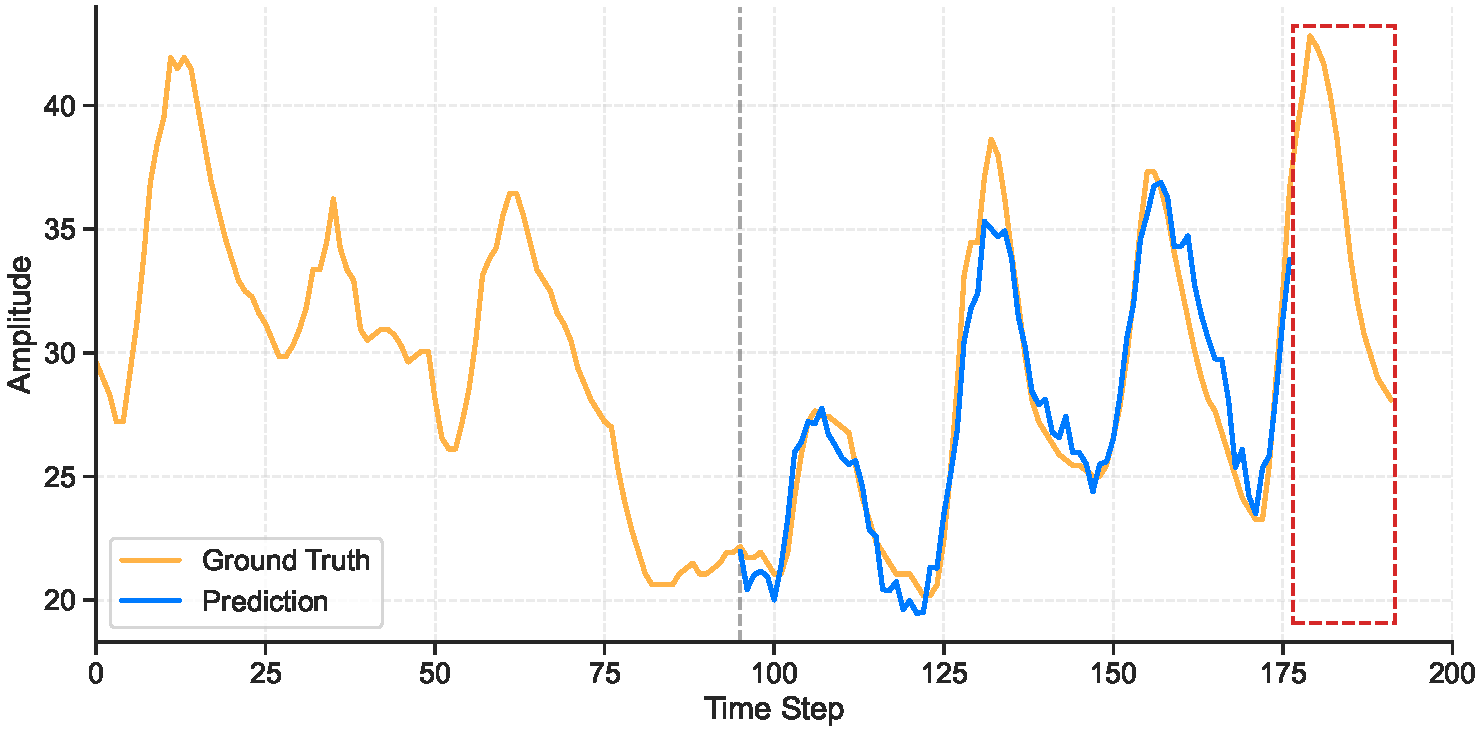
\includegraphics[width=\linewidth]{figures/appendix/showcase_additional/ground_truth_plot_01_len.pdf}\caption{Incomplete prediction (early stopping).}\label{fig:showcase01_add01-len}\end{subfigure}%
\hfill%
\begin{subfigure}[t]{0.32\linewidth}\centering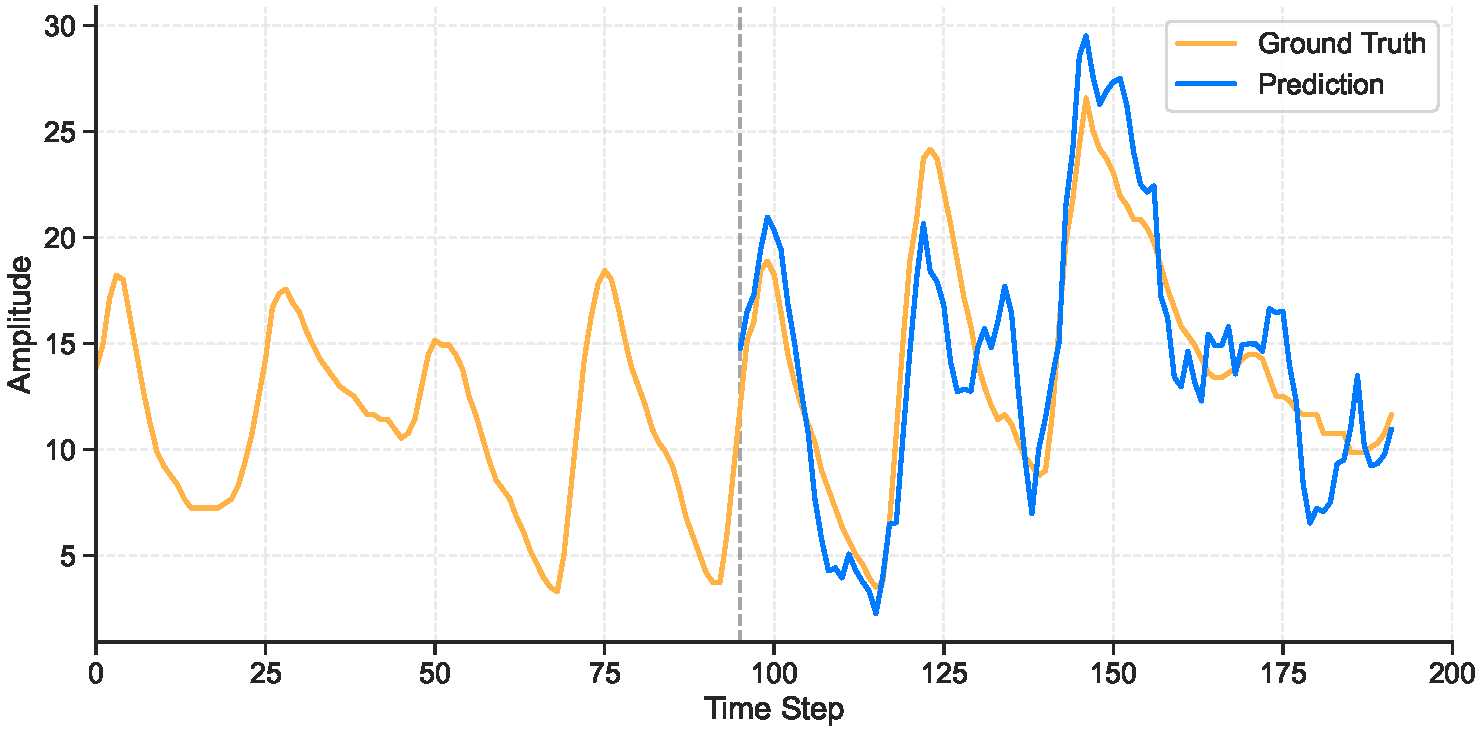
\includegraphics[width=\linewidth]{figures/appendix/showcase_additional/ground_truth_plot_02_mse.pdf}\caption{Low prediction accuracy (high MSE).}\label{fig:showcase02_add01-mse}\end{subfigure}%
\hfill%
\begin{subfigure}[t]{0.32\linewidth}\centering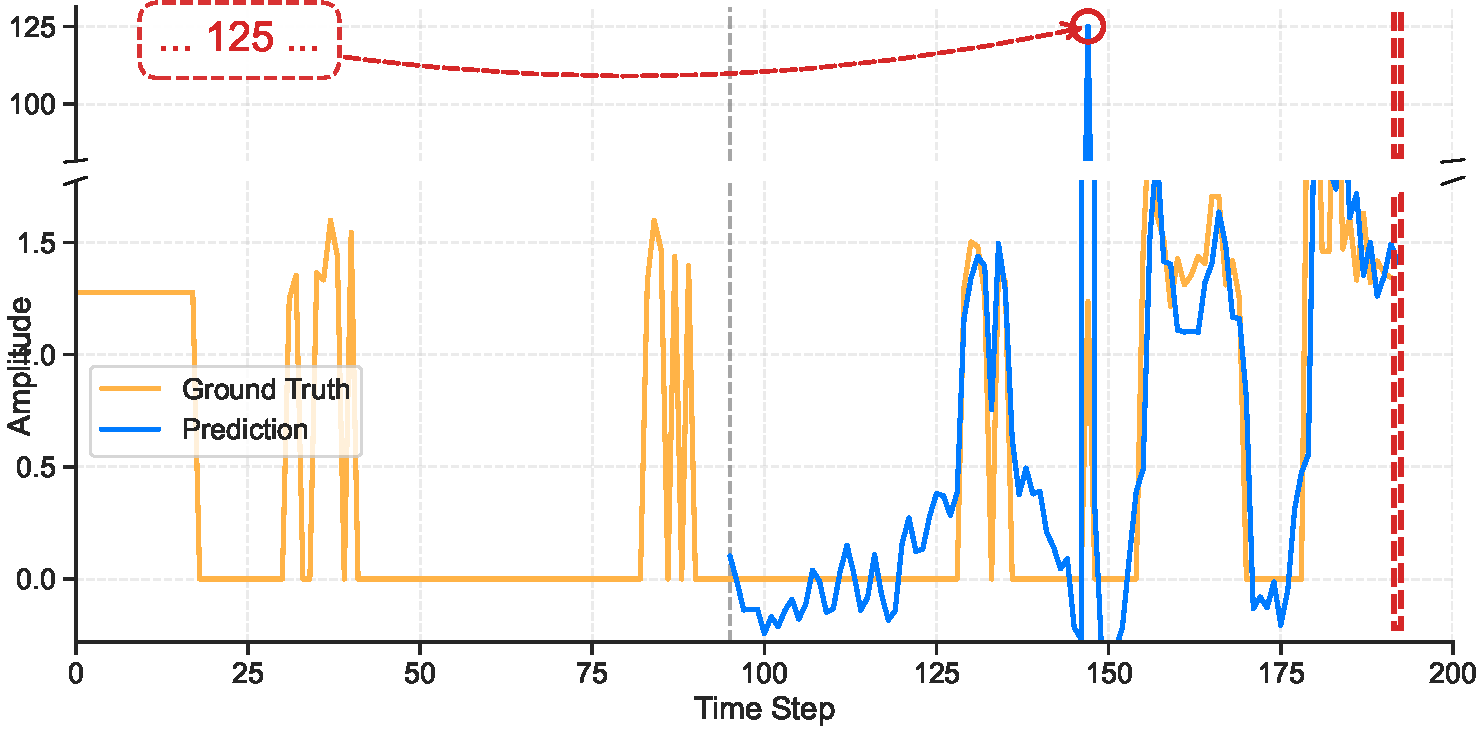
\includegraphics[width=\linewidth]{figures/appendix/showcase_additional/ground_truth_plot_03_decimal.pdf}\caption{Formatting error causing abnormal spikes.}\label{fig:showcase03_add01-fmt}\end{subfigure}%
\par\medskip
\begin{subfigure}[t]{0.32\linewidth}\centering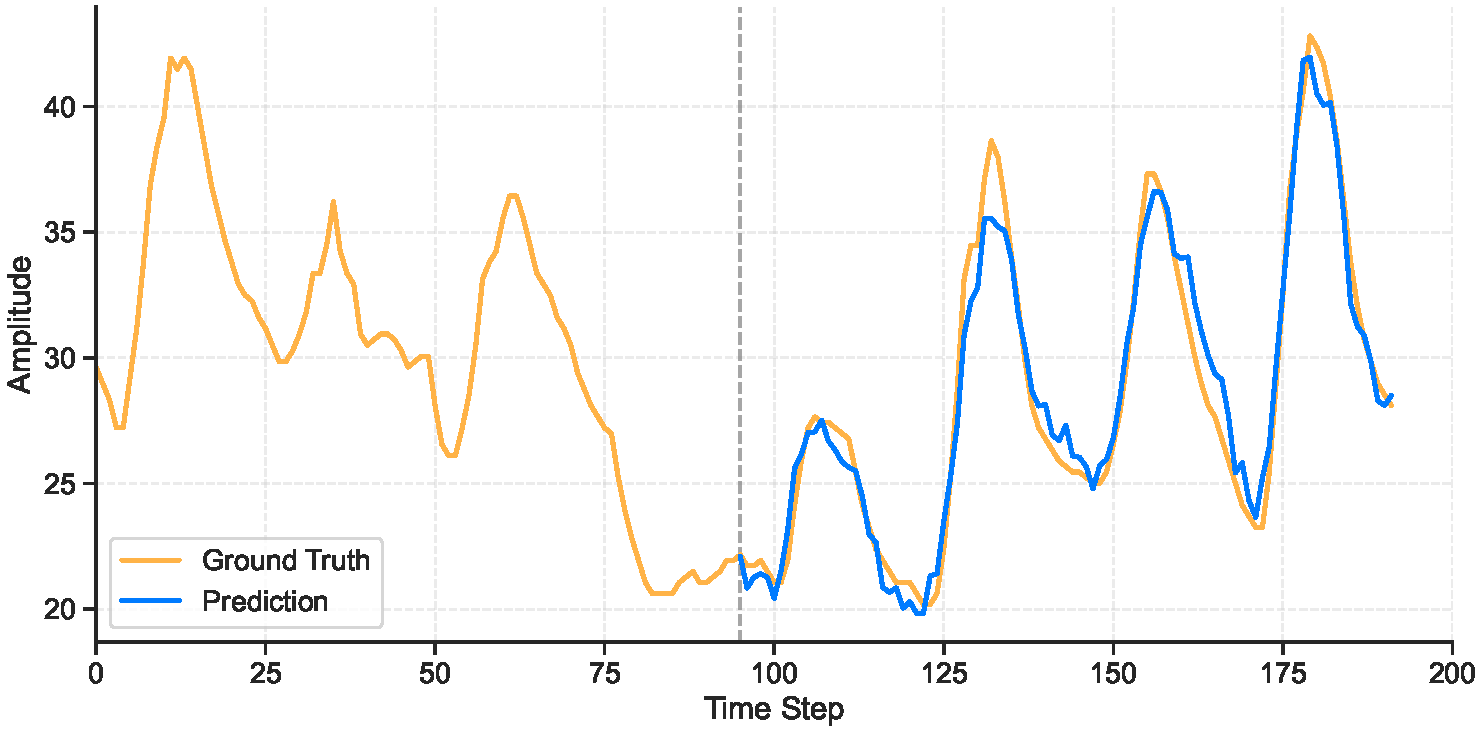
\includegraphics[width=\linewidth]{figures/appendix/showcase_additional/ground_truth_plot_01.pdf}\caption{Correction of prediction length.}\label{fig:showcase01_add01}\end{subfigure}%
\hfill%
\begin{subfigure}[t]{0.32\linewidth}\centering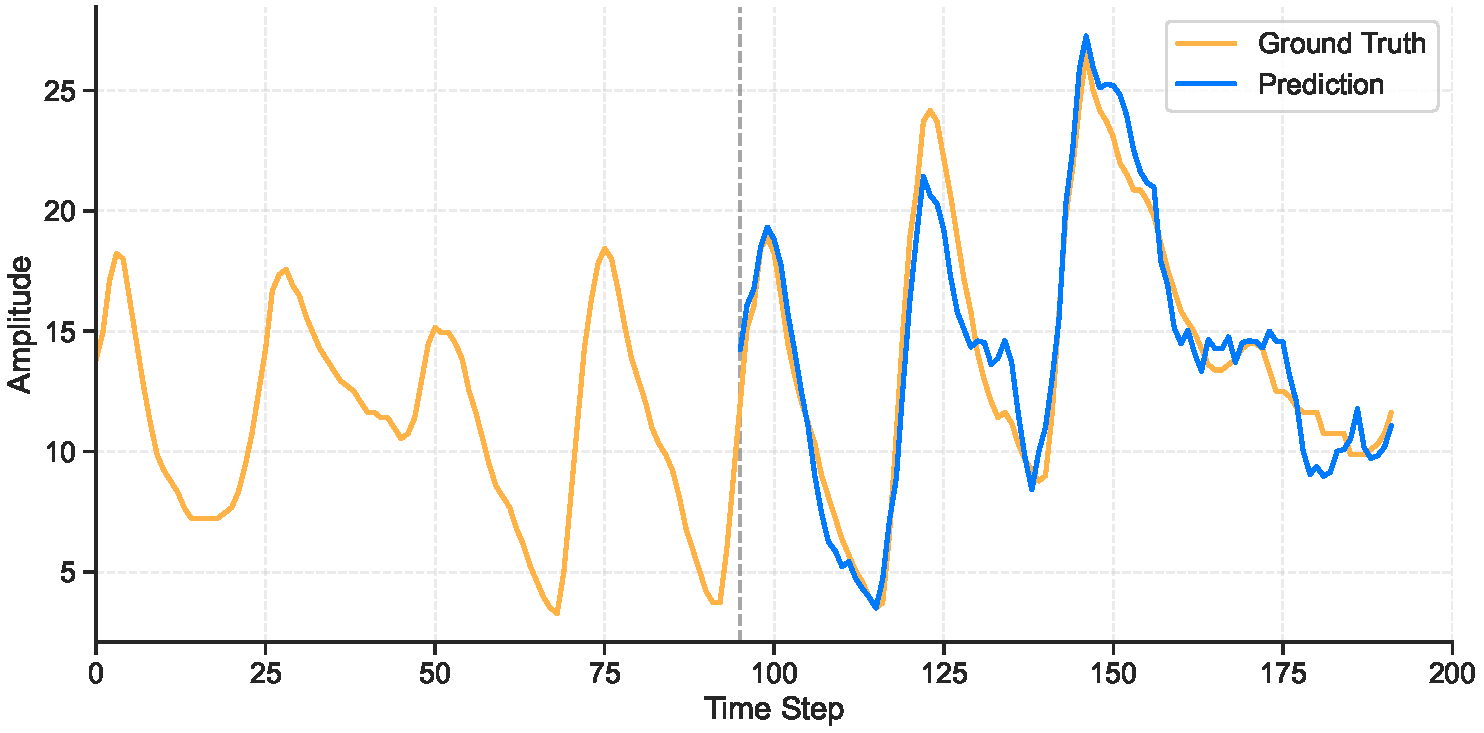
\includegraphics[width=\linewidth]{figures/appendix/showcase_additional/ground_truth_plot_02.pdf}\caption{Enhanced prediction precision.}\label{fig:showcase02_add01}\end{subfigure}%
\hfill%
\begin{subfigure}[t]{0.32\linewidth}\centering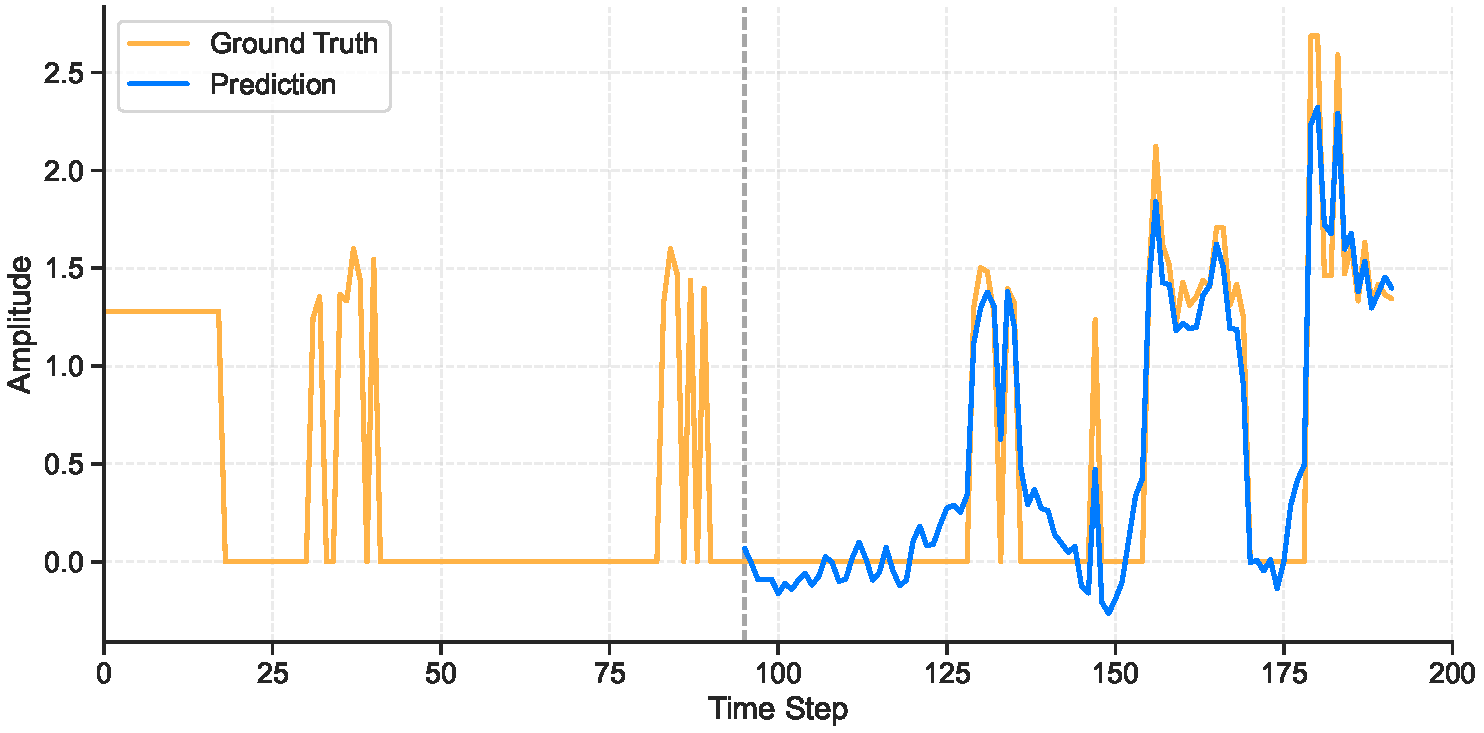
\includegraphics[width=\linewidth]{figures/appendix/showcase_additional/ground_truth_plot_03.pdf}\caption{Rectification of output format and outliers.}\label{fig:showcase03_add01}\end{subfigure}%

\caption{More showcases visualization of input-96-predict-96 results on the ETTh2 dataset. The top row (a-c) displays the baseline performance of the STIT model, which exhibits limitations in sequence length, accuracy, and output formatting. The bottom row (d-f) showcases the improvements achieved after applying the proposed RDFR framework on the corresponding samples.}\label{fig:showcases_add_01}\end{figure}


\input{figures/appendix/showcase_additional/showcase_additional_02}

\FloatBarrier\needspace{10\baselineskip}

\section{Prompt}\label{appx:prompt}

This appendix details the specific prompt designs employed in our experiment.

\begingroup\raggedright\refstepcounter{figure}

    \begin{chatbox}{Dialogue Example: Time Series Forecasting}
        \userbt{
        You are a multivariate time series forecasting expert, and you are conducting a multivariate time series forecasting task. Variables include HUFL (High Useful Load), HULL (High Useless Load), MUFL (Middle Useful Load), MULL (Middle Useless Load), LUFL (Low Useful Load), LULL (Low Useless Load), and OT (Oil Temperature). The current time is 2016-07-09 02:00:00, and here are 96 historical data points:  \\

        2016-07-05 03:00:00,
        10.717000007629396,
        5.425000190734863,
        8.065999984741211,
        2.878000020980835,
        2.8329999446868896,
        1.8580000400543213,
        28.913000106811523 \\
        2016-07-05 04:00:00,
        11.31999969482422,
        5.625999927520752,
        7.676000118255615,
        2.630000114440918,
        3.0460000038146973,
        1.888000011444092,
        30.459999084472656 \\
        2016-07-05 05:00:00,
        10.85099983215332,
        4.689000129699707,
        6.822999954223633,
        1.883000016212464,
        3.3199999332427983,
        2.0409998893737797,
        31.3750009442556968, \\

        ...... \\

        2016-07-09  00:00:00,
        14.60200023651123,
        5.960999965667725,
        11.300000190734865,
        3.3399999141693115,
        3.259000062942505,
        1.7669999599456787,
        30.952999114990234 \\
        2016-07-09 01:00:00,
        14.53499984741211,
        6.162000179290772,
        11.690999984741213,
        3.908999919891357,
        3.0460000038146973,
        1.6449999809265137,
        30.31999969482422 \\
        2016-07-09 02:00:00,
        14.401000022888185,
        6.296000003814697,
        11.72700023651123,
        3.9440000057220463,
        2.8020000457763667,
        1.6139999628067017,
        29.40500068664551 \\
        Predict all variables for the next 96 data points. \\
        }

        \smallskip

        \agentbt{
        Here are next 96 predictions, \\
        2016-07-09 03:00:00, 13.8761189064844679, 6.2196899796516814, 11.2944295697469368, 4.2530431436381280, 2.1881263437365770, 1.2201847471905527, 28.9887656946704766 \\
        2016-07-09 04:00:00, 14.2560721512361734, 5.9231297870012867, 11.4640511170778296, 4.7462475899091974, 2.9999912251093641, 1.0527562380645918, 28.4748593490313695 \\
        2016-07-09 05:00:00, 14.7053675264032115, 5.4290932353666825, 11.5004855354919862, 4.9681193018049274, 2.9424307768411118, 0.5318665943402617, 28.9633890297951275 \\
        2016-07-09 06:00:00, 15.0472919700687022, 6.1630397546891587, 11.1093843098066891, 4.6707001161588977, 2.6000304425794396, 0.3997434904746003, 29.3292634695356469 \\
        2016-07-09 07:00:00, 14.2812091330150857, 6.3270099694262933, 12.3872873810183677, 4.6466697713273275, 2.3947366181772844, 0.1303528815588440, 29.4522558724904258 \\
        ...... \\
        2016-07-11 00:00:00, 16.8784257408377023, 5.0188430039810648, 5.1576691434726314, 3.9998658250940680, 3.2536048105448589, 3.6541286210987103, 30.6599944851329909 \\
        2016-07-11 01:00:00, 17.2443990451752711, 5.3244076172971182, 4.9414113159207771, 3.7657028289748924, 2.5107311848805542, 3.0150452718955765, 30.5161683922856284 \\
        2016-07-11 02:00:00, 16.6936500560171659, 5.2596094859684186, 4.8941272400060143, 2.8417151584125859, 2.2165416340952087, 2.5979149027470849, 30.9421436418460551 \\
        }
    \end{chatbox}
    \par\smallskip\noindent\textit{Figure \thefigure. A representative dialogue showing the user prompt and model response.}
    \label{fig:dialogue_example}
\par\endgroup


\FloatBarrier\needspace{10\baselineskip}\section{Societal Impacts}
The proposed RDTU framework has the potential to benefit a wide range of real-world forecasting applications, such as energy management, transportation planning, finance, weather analysis, and public-resource allocation. By simplifying LLM-based time series forecasting without relying on complex pre-alignment modules, the framework may lower the engineering barrier for adapting foundation models to temporal prediction tasks and improve forecasting accessibility in data-limited scenarios. More accurate and generalizable forecasts can support better planning, reduce resource waste, and improve the reliability of decision-making systems. At the same time, as with other forecasting methods, inaccurate predictions may lead to suboptimal decisions if the model is deployed without proper validation. Therefore, practical use of the proposed framework should include domain-specific validation when applied to sensitive real-world decision-making scenarios.

\section*{Source and formatting notes}\addcontentsline{toc}{section}{Source and formatting notes}
The full-manuscript source is the basis for all numerical values in this supplement. Existing summary averages, source-reported rank-count footers and statistical values are retained as supplied; the repository's source notes identify inconsistencies in those summaries. No experiments were rerun when preparing this material. The historical novelty wording was aligned with the final manuscript's narrower description of the method. The NeurIPS conference checklist author responses are archived in the repository separately from the research material; template instructions and placeholder author information are excluded.
\clearpage\bibliographystyle{plainnat}\bibliography{reference}\end{document}
